%% fig_signature.tex   (generated by make_diagrams.py; do not edit by hand)
%% The signatures (p,q) of an imaginary quadratic action on the surface of height pq, with the Weil ridge p = q.
\documentclass[tikz,border=8pt]{standalone}
\usepackage{amsmath,amssymb}
\usetikzlibrary{arrows.meta,calc}
%% palette.tex -- shared colour definitions for the figures
\definecolor{PInk}{RGB}{26,32,44}
\definecolor{PBlue}{RGB}{37,82,139}
\definecolor{PTeal}{RGB}{23,127,125}
\definecolor{POchre}{RGB}{193,138,44}
\definecolor{PClay}{RGB}{178,74,58}
\definecolor{PSlate}{RGB}{108,122,137}
\definecolor{PViolet}{RGB}{110,86,150}
\definecolor{WBlue}{RGB}{223,234,246}
\definecolor{WTeal}{RGB}{220,238,236}
\definecolor{WOchre}{RGB}{250,240,218}
\definecolor{WClay}{RGB}{247,229,224}
\definecolor{WSlate}{RGB}{238,241,244}
\definecolor{PMag}{RGB}{158,58,110}
\definecolor{PGrass}{RGB}{62,124,66}
\definecolor{PAmber}{RGB}{214,112,38}
\definecolor{PIndigo}{RGB}{58,64,140}
\definecolor{PRule}{RGB}{176,186,197}

%% shared macros so the standalone figures match the paper
\providecommand{\QQ}{\mathbb{Q}}
\providecommand{\ZZ}{\mathbb{Z}}
\providecommand{\RR}{\mathbb{R}}
\providecommand{\CC}{\mathbb{C}}
\providecommand{\PP}{\mathbb{P}}
\providecommand{\Kx}{K^{\times}}
\providecommand{\HW}{W}
\providecommand{\Nm}{\mathrm{N}}
\providecommand{\Hdg}{\mathrm{Hdg}}
\providecommand{\NS}{\mathrm{NS}}
\providecommand{\cA}{\mathcal{A}}
\providecommand{\cD}{\mathcal{D}}
\providecommand{\cF}{\mathcal{F}}
\providecommand{\cP}{\mathcal{P}}
\providecommand{\cO}{\mathcal{O}}
\providecommand{\cQ}{\mathcal{Q}}
\providecommand{\bbar}[1]{\overline{#1}}
\providecommand{\ch}{\operatorname{ch}}
\providecommand{\End}{\mathrm{End}}

\begin{document}
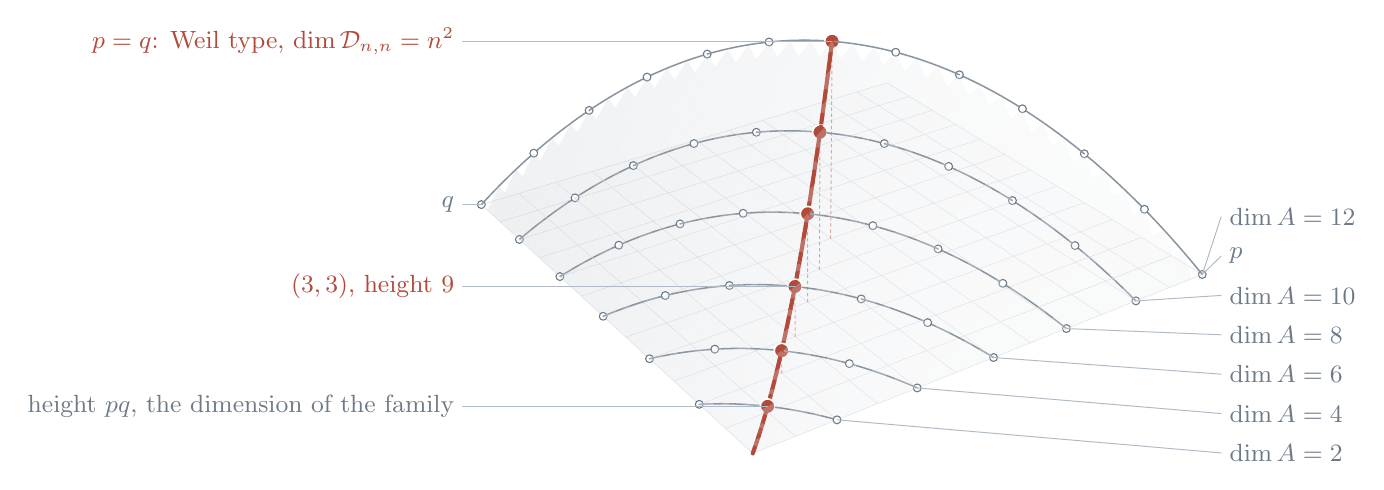
\begin{tikzpicture}[x=1cm,y=1cm,line join=round,line cap=round,
  font=\small,text=PInk]
  \path[draw=none,fill opacity=0.10,fill=PSlate!16!white] (0.9655,1.3937) -- (1.2226,1.4719) -- (1.0352,1.5858) -- (0.7792,1.5091) -- cycle;
  \path[draw=none,fill opacity=0.10,fill=PSlate!16!white] (0.7051,1.3145) -- (0.9655,1.3937) -- (0.7792,1.5091) -- (0.5201,1.4313) -- cycle;
  \path[draw=none,fill opacity=0.10,fill=PSlate!16!white] (1.1552,1.2762) -- (1.4135,1.3559) -- (1.2226,1.4719) -- (0.9655,1.3937) -- cycle;
  \path[draw=none,fill opacity=0.10,fill=PSlate!16!white] (0.4414,1.2343) -- (0.7051,1.3145) -- (0.5201,1.4313) -- (0.2577,1.3526) -- cycle;
  \path[draw=none,fill opacity=0.10,fill=PSlate!16!white] (0.8936,1.1955) -- (1.1552,1.2762) -- (0.9655,1.3937) -- (0.7051,1.3145) -- cycle;
  \path[draw=none,fill opacity=0.10,fill=PSlate!16!white] (1.3486,1.1565) -- (1.6081,1.2376) -- (1.4135,1.3559) -- (1.1552,1.2762) -- cycle;
  \path[draw=none,fill opacity=0.10,fill=PSlate!16!white] (0.1743,1.1531) -- (0.4414,1.2343) -- (0.2577,1.3526) -- (-0.0080,1.2729) -- cycle;
  \path[draw=none,fill opacity=0.10,fill=PSlate!16!white] (0.6286,1.1138) -- (0.8936,1.1955) -- (0.7051,1.3145) -- (0.4414,1.2343) -- cycle;
  \path[draw=none,fill opacity=0.10,fill=PSlate!16!white] (1.0857,1.0742) -- (1.3486,1.1565) -- (1.1552,1.2762) -- (0.8936,1.1955) -- cycle;
  \path[draw=none,fill opacity=0.10,fill=PSlate!16!white] (-0.0962,1.0708) -- (0.1743,1.1531) -- (-0.0080,1.2729) -- (-0.2772,1.1922) -- cycle;
  \path[draw=none,fill opacity=0.10,fill=PSlate!16!white] (1.5456,1.0344) -- (1.8063,1.1172) -- (1.6081,1.2376) -- (1.3486,1.1565) -- cycle;
  \path[draw=none,fill opacity=0.10,fill=PSlate!16!white] (0.3602,1.0310) -- (0.6286,1.1138) -- (0.4414,1.2343) -- (0.1743,1.1531) -- cycle;
  \path[draw=none,fill opacity=0.10,fill=PSlate!16!white] (0.8194,0.9909) -- (1.0857,1.0742) -- (0.8936,1.1955) -- (0.6286,1.1138) -- cycle;
  \path[draw=none,fill opacity=0.10,fill=PSlate!16!white] (-0.3702,0.9875) -- (-0.0962,1.0708) -- (-0.2772,1.1922) -- (-0.5498,1.1104) -- cycle;
  \path[draw=none,fill opacity=0.10,fill=PSlate!16!white] (1.2815,0.9506) -- (1.5456,1.0344) -- (1.3486,1.1565) -- (1.0857,1.0742) -- cycle;
  \path[draw=none,fill opacity=0.10,fill=PSlate!16!white] (0.0882,0.9471) -- (0.3602,1.0310) -- (0.1743,1.1531) -- (-0.0962,1.0708) -- cycle;
  \path[draw=none,fill opacity=0.10,fill=PSlate!16!white] (1.7464,0.9100) -- (2.0084,0.9944) -- (1.8063,1.1172) -- (1.5456,1.0344) -- cycle;
  \path[draw=none,fill opacity=0.10,fill=PSlate!16!white] (0.5496,0.9065) -- (0.8194,0.9909) -- (0.6286,1.1138) -- (0.3602,1.0310) -- cycle;
  \path[draw=none,fill opacity=0.10,fill=PSlate!16!white] (-0.6479,0.9030) -- (-0.3702,0.9875) -- (-0.5498,1.1104) -- (-0.8259,1.0276) -- cycle;
  \path[draw=none,fill opacity=0.10,fill=PSlate!16!white] (1.0139,0.8657) -- (1.2815,0.9506) -- (1.0857,1.0742) -- (0.8194,0.9909) -- cycle;
  \path[draw=none,fill opacity=0.10,fill=PSlate!16!white] (-0.1872,0.8622) -- (0.0882,0.9471) -- (-0.0962,1.0708) -- (-0.3702,0.9875) -- cycle;
  \path[draw=none,fill opacity=0.10,fill=PSlate!16!white] (1.4811,0.8246) -- (1.7464,0.9100) -- (1.5456,1.0344) -- (1.2815,0.9506) -- cycle;
  \path[draw=none,fill opacity=0.10,fill=PSlate!16!white] (0.2763,0.8210) -- (0.5496,0.9065) -- (0.3602,1.0310) -- (0.0882,0.9471) -- cycle;
  \path[draw=none,fill opacity=0.10,fill=PSlate!16!white] (-0.9291,0.8175) -- (-0.6479,0.9030) -- (-0.8259,1.0276) -- (-1.1056,0.9437) -- cycle;
  \path[draw=none,fill opacity=0.10,fill=PSlate!16!white] (1.9512,0.7832) -- (2.2143,0.8692) -- (2.0084,0.9944) -- (1.7464,0.9100) -- cycle;
  \path[draw=none,fill opacity=0.10,fill=PSlate!16!white] (0.7427,0.7796) -- (1.0139,0.8657) -- (0.8194,0.9909) -- (0.5496,0.9065) -- cycle;
  \path[draw=none,fill opacity=0.10,fill=PSlate!16!white] (-0.4664,0.7761) -- (-0.1872,0.8622) -- (-0.3702,0.9875) -- (-0.6479,0.9030) -- cycle;
  \draw[PRule!50,line width=0.15pt] (-4.1171,0.0403) -- (1.0352,1.5858);
  \path[draw=none,fill opacity=0.10,fill=PSlate!16!white] (1.2122,0.7380) -- (1.4811,0.8246) -- (1.2815,0.9506) -- (1.0139,0.8657) -- cycle;
  \path[draw=none,fill opacity=0.10,fill=PSlate!16!white] (-0.0006,0.7344) -- (0.2763,0.8210) -- (0.0882,0.9471) -- (-0.1872,0.8622) -- cycle;
  \path[draw=none,fill opacity=0.10,fill=PSlate!16!white] (-1.2141,0.7308) -- (-0.9291,0.8175) -- (-1.1056,0.9437) -- (-1.3890,0.8586) -- cycle;
  \path[draw=none,fill opacity=0.10,fill=PSlate!16!white] (1.6846,0.6961) -- (1.9512,0.7832) -- (1.7464,0.9100) -- (1.4811,0.8246) -- cycle;
  \path[draw=none,fill opacity=0.10,fill=PSlate!16!white] (0.4680,0.6925) -- (0.7427,0.7796) -- (0.5496,0.9065) -- (0.2763,0.8210) -- cycle;
  \path[draw=none,fill opacity=0.10,fill=PSlate!16!white] (-0.7492,0.6889) -- (-0.4664,0.7761) -- (-0.6479,0.9030) -- (-0.9291,0.8175) -- cycle;
  \path[draw=none,fill opacity=0.10,fill=PSlate!16!white] (2.1600,0.6539) -- (2.4243,0.7416) -- (2.2143,0.8692) -- (1.9512,0.7832) -- cycle;
  \path[draw=none,fill opacity=0.10,fill=PSlate!16!white] (0.9397,0.6502) -- (1.2122,0.7380) -- (1.0139,0.8657) -- (0.7427,0.7796) -- cycle;
  \path[draw=none,fill opacity=0.10,fill=PSlate!16!white] (-0.2813,0.6466) -- (-0.0006,0.7344) -- (-0.1872,0.8622) -- (-0.4664,0.7761) -- cycle;
  \path[draw=none,fill opacity=0.10,fill=PSlate!16!white] (-1.5029,0.6430) -- (-1.2141,0.7308) -- (-1.3890,0.8586) -- (-1.6761,0.7725) -- cycle;
  \path[draw=none,fill opacity=0.10,fill=PSlate!16!white] (1.4144,0.6078) -- (1.6846,0.6961) -- (1.4811,0.8246) -- (1.2122,0.7380) -- cycle;
  \path[draw=none,fill opacity=0.10,fill=PSlate!16!white] (0.1896,0.6041) -- (0.4680,0.6925) -- (0.2763,0.8210) -- (-0.0006,0.7344) -- cycle;
  \path[draw=none,fill opacity=0.10,fill=PSlate!16!white] (-1.0358,0.6005) -- (-0.7492,0.6889) -- (-0.9291,0.8175) -- (-1.2141,0.7308) -- cycle;
  \path[draw=none,fill opacity=0.10,fill=PSlate!16!white] (1.8921,0.5650) -- (2.1600,0.6539) -- (1.9512,0.7832) -- (1.6846,0.6961) -- cycle;
  \path[draw=none,fill opacity=0.10,fill=PSlate!16!white] (0.6636,0.5613) -- (0.9397,0.6502) -- (0.7427,0.7796) -- (0.4680,0.6925) -- cycle;
  \path[draw=none,fill opacity=0.10,fill=PSlate!16!white] (-0.5657,0.5577) -- (-0.2813,0.6466) -- (-0.4664,0.7761) -- (-0.7492,0.6889) -- cycle;
  \draw[PRule!50,line width=0.15pt] (-3.8796,-0.1776) -- (1.3176,1.4142);
  \path[draw=none,fill opacity=0.10,fill=PSlate!16!white] (-1.7956,0.5540) -- (-1.5029,0.6430) -- (-1.6761,0.7725) -- (-1.9671,0.6852) -- cycle;
  \path[draw=none,fill opacity=0.10,fill=PSlate!16!white] (2.3729,0.5220) -- (2.6385,0.6114) -- (2.4243,0.7416) -- (2.1600,0.6539) -- cycle;
  \path[draw=none,fill opacity=0.10,fill=PSlate!16!white] (1.1406,0.5183) -- (1.4144,0.6078) -- (1.2122,0.7380) -- (0.9397,0.6502) -- cycle;
  \path[draw=none,fill opacity=0.10,fill=PSlate!16!white] (-0.0925,0.5146) -- (0.1896,0.6041) -- (-0.0006,0.7344) -- (-0.2813,0.6466) -- cycle;
  \path[draw=none,fill opacity=0.10,fill=PSlate!16!white] (-1.3263,0.5109) -- (-1.0358,0.6005) -- (-1.2141,0.7308) -- (-1.5029,0.6430) -- cycle;
  \path[draw=none,fill opacity=0.10,fill=PSlate!16!white] (1.6206,0.4749) -- (1.8921,0.5650) -- (1.6846,0.6961) -- (1.4144,0.6078) -- cycle;
  \path[draw=none,fill opacity=0.10,fill=PSlate!16!white] (0.3837,0.4712) -- (0.6636,0.5613) -- (0.4680,0.6925) -- (0.1896,0.6041) -- cycle;
  \path[draw=none,fill opacity=0.10,fill=PSlate!16!white] (-0.8539,0.4675) -- (-0.5657,0.5577) -- (-0.7492,0.6889) -- (-1.0358,0.6005) -- cycle;
  \path[draw=none,fill opacity=0.10,fill=PSlate!16!white] (-2.0922,0.4638) -- (-1.7956,0.5540) -- (-1.9671,0.6852) -- (-2.2619,0.5968) -- cycle;
  \path[draw=none,fill opacity=0.10,fill=PSlate!16!white] (2.1038,0.4313) -- (2.3729,0.5220) -- (2.1600,0.6539) -- (1.8921,0.5650) -- cycle;
  \path[draw=none,fill opacity=0.10,fill=PSlate!16!white] (0.8630,0.4276) -- (1.1406,0.5183) -- (0.9397,0.6502) -- (0.6636,0.5613) -- cycle;
  \path[draw=none,fill opacity=0.10,fill=PSlate!16!white] (-0.3785,0.4238) -- (-0.0925,0.5146) -- (-0.2813,0.6466) -- (-0.5657,0.5577) -- cycle;
  \path[draw=none,fill opacity=0.10,fill=PSlate!16!white] (-1.6207,0.4201) -- (-1.3263,0.5109) -- (-1.5029,0.6430) -- (-1.7956,0.5540) -- cycle;
  \path[draw=none,fill opacity=0.10,fill=PSlate!16!white] (2.5902,0.3874) -- (2.8569,0.4787) -- (2.6385,0.6114) -- (2.3729,0.5220) -- cycle;
  \path[draw=none,fill opacity=0.10,fill=PSlate!16!white] (1.3455,0.3837) -- (1.6206,0.4749) -- (1.4144,0.6078) -- (1.1406,0.5183) -- cycle;
  \path[draw=none,fill opacity=0.10,fill=PSlate!16!white] (0.1001,0.3799) -- (0.3837,0.4712) -- (0.1896,0.6041) -- (-0.0925,0.5146) -- cycle;
  \path[draw=none,fill opacity=0.10,fill=PSlate!16!white] (-1.1460,0.3761) -- (-0.8539,0.4675) -- (-1.0358,0.6005) -- (-1.3263,0.5109) -- cycle;
  \path[draw=none,fill opacity=0.10,fill=PSlate!16!white] (-2.3928,0.3723) -- (-2.0922,0.4638) -- (-2.2619,0.5968) -- (-2.5607,0.5072) -- cycle;
  \draw[PRule!50,line width=0.15pt] (5.0382,-0.8471) -- (1.0352,1.5858);
  \draw[PRule!50,line width=0.15pt] (-3.6345,-0.4023) -- (1.6081,1.2376);
  \path[draw=none,fill opacity=0.10,fill=PSlate!16!white] (1.8311,0.3394) -- (2.1038,0.4313) -- (1.8921,0.5650) -- (1.6206,0.4749) -- cycle;
  \path[draw=none,fill opacity=0.10,fill=PSlate!16!white] (0.5817,0.3356) -- (0.8630,0.4276) -- (0.6636,0.5613) -- (0.3837,0.4712) -- cycle;
  \path[draw=none,fill opacity=0.10,fill=PSlate!16!white] (-0.6683,0.3318) -- (-0.3785,0.4238) -- (-0.5657,0.5577) -- (-0.8539,0.4675) -- cycle;
  \path[draw=none,fill opacity=0.10,fill=PSlate!16!white] (-1.9191,0.3280) -- (-1.6207,0.4201) -- (-1.7956,0.5540) -- (-2.0922,0.4638) -- cycle;
  \path[draw=none,fill opacity=0.10,fill=PSlate!16!white] (2.3198,0.2949) -- (2.5902,0.3874) -- (2.3729,0.5220) -- (2.1038,0.4313) -- cycle;
  \path[draw=none,fill opacity=0.10,fill=PSlate!16!white] (1.0665,0.2911) -- (1.3455,0.3837) -- (1.1406,0.5183) -- (0.8630,0.4276) -- cycle;
  \path[draw=none,fill opacity=0.10,fill=PSlate!16!white] (-0.1875,0.2873) -- (0.1001,0.3799) -- (-0.0925,0.5146) -- (-0.3785,0.4238) -- cycle;
  \path[draw=none,fill opacity=0.10,fill=PSlate!16!white] (-1.4422,0.2835) -- (-1.1460,0.3761) -- (-1.3263,0.5109) -- (-1.6207,0.4201) -- cycle;
  \path[draw=none,fill opacity=0.10,fill=PSlate!16!white] (-2.6976,0.2796) -- (-2.3928,0.3723) -- (-2.5607,0.5072) -- (-2.8635,0.4163) -- cycle;
  \path[draw=none,fill opacity=0.10,fill=PSlate!16!white] (2.8118,0.2502) -- (3.0797,0.3432) -- (2.8569,0.4787) -- (2.5902,0.3874) -- cycle;
  \path[draw=none,fill opacity=0.10,fill=PSlate!16!white] (1.5545,0.2463) -- (1.8311,0.3394) -- (1.6206,0.4749) -- (1.3455,0.3837) -- cycle;
  \path[draw=none,fill opacity=0.10,fill=PSlate!16!white] (0.2965,0.2424) -- (0.5817,0.3356) -- (0.3837,0.4712) -- (0.1001,0.3799) -- cycle;
  \path[draw=none,fill opacity=0.10,fill=PSlate!16!white] (-0.9622,0.2386) -- (-0.6683,0.3318) -- (-0.8539,0.4675) -- (-1.1460,0.3761) -- cycle;
  \path[draw=none,fill opacity=0.10,fill=PSlate!16!white] (-2.2216,0.2347) -- (-1.9191,0.3280) -- (-2.0922,0.4638) -- (-2.3928,0.3723) -- cycle;
  \draw[PRule!50,line width=0.15pt] (4.6213,-1.0130) -- (0.6501,1.4703);
  \path[draw=none,fill opacity=0.10,fill=PSlate!16!white] (2.0458,0.2012) -- (2.3198,0.2949) -- (2.1038,0.4313) -- (1.8311,0.3394) -- cycle;
  \path[draw=none,fill opacity=0.10,fill=PSlate!16!white] (0.7837,0.1973) -- (1.0665,0.2911) -- (0.8630,0.4276) -- (0.5817,0.3356) -- cycle;
  \path[draw=none,fill opacity=0.10,fill=PSlate!16!white] (-0.4790,0.1934) -- (-0.1875,0.2873) -- (-0.3785,0.4238) -- (-0.6683,0.3318) -- cycle;
  \path[draw=none,fill opacity=0.10,fill=PSlate!16!white] (-1.7424,0.1895) -- (-1.4422,0.2835) -- (-1.6207,0.4201) -- (-1.9191,0.3280) -- cycle;
  \path[draw=none,fill opacity=0.10,fill=PSlate!16!white] (-3.0066,0.1857) -- (-2.6976,0.2796) -- (-2.8635,0.4163) -- (-3.1705,0.3242) -- cycle;
  \path[draw=none,fill opacity=0.10,fill=PSlate!16!white] (2.5402,0.1558) -- (2.8118,0.2502) -- (2.5902,0.3874) -- (2.3198,0.2949) -- cycle;
  \path[draw=none,fill opacity=0.10,fill=PSlate!16!white] (1.2742,0.1519) -- (1.5545,0.2463) -- (1.3455,0.3837) -- (1.0665,0.2911) -- cycle;
  \path[draw=none,fill opacity=0.10,fill=PSlate!16!white] (0.0074,0.1480) -- (0.2965,0.2424) -- (0.1001,0.3799) -- (-0.1875,0.2873) -- cycle;
  \draw[PRule!50,line width=0.15pt] (-3.3814,-0.6344) -- (1.9069,1.0561);
  \path[draw=none,fill opacity=0.10,fill=PSlate!16!white] (-1.2601,0.1440) -- (-0.9622,0.2386) -- (-1.1460,0.3761) -- (-1.4422,0.2835) -- cycle;
  \path[draw=none,fill opacity=0.10,fill=PSlate!16!white] (-2.5283,0.1401) -- (-2.2216,0.2347) -- (-2.3928,0.3723) -- (-2.6976,0.2796) -- cycle;
  \path[draw=none,fill opacity=0.10,fill=PSlate!16!white] (3.0380,0.1101) -- (3.3071,0.2051) -- (3.0797,0.3432) -- (2.8118,0.2502) -- cycle;
  \path[draw=none,fill opacity=0.10,fill=PSlate!16!white] (1.7679,0.1061) -- (2.0458,0.2012) -- (1.8311,0.3394) -- (1.5545,0.2463) -- cycle;
  \path[draw=none,fill opacity=0.10,fill=PSlate!16!white] (0.4970,0.1022) -- (0.7837,0.1973) -- (0.5817,0.3356) -- (0.2965,0.2424) -- cycle;
  \path[draw=none,fill opacity=0.10,fill=PSlate!16!white] (-0.7745,0.0983) -- (-0.4790,0.1934) -- (-0.6683,0.3318) -- (-0.9622,0.2386) -- cycle;
  \path[draw=none,fill opacity=0.10,fill=PSlate!16!white] (-2.0468,0.0943) -- (-1.7424,0.1895) -- (-1.9191,0.3280) -- (-2.2216,0.2347) -- cycle;
  \path[draw=none,fill opacity=0.10,fill=PSlate!16!white] (-3.3198,0.0904) -- (-3.0066,0.1857) -- (-3.1705,0.3242) -- (-3.4817,0.2309) -- cycle;
  \draw[PRule!50,line width=0.15pt] (4.1948,-1.1827) -- (0.2577,1.3526);
  \path[draw=none,fill opacity=0.10,fill=PSlate!16!white] (2.2649,0.0601) -- (2.5402,0.1558) -- (2.3198,0.2949) -- (2.0458,0.2012) -- cycle;
  \path[draw=none,fill opacity=0.10,fill=PSlate!16!white] (0.9899,0.0561) -- (1.2742,0.1519) -- (1.0665,0.2911) -- (0.7837,0.1973) -- cycle;
  \path[draw=none,fill opacity=0.10,fill=PSlate!16!white] (-0.2857,0.0522) -- (0.0074,0.1480) -- (-0.1875,0.2873) -- (-0.4790,0.1934) -- cycle;
  \path[draw=none,fill opacity=0.10,fill=PSlate!16!white] (-1.5621,0.0482) -- (-1.2601,0.1440) -- (-1.4422,0.2835) -- (-1.7424,0.1895) -- cycle;
  \path[draw=none,fill opacity=0.10,fill=PSlate!16!white] (-2.8393,0.0442) -- (-2.5283,0.1401) -- (-2.6976,0.2796) -- (-3.0066,0.1857) -- cycle;
  \path[draw=none,fill opacity=0.10,fill=PSlate!16!white] (2.7652,0.0137) -- (3.0380,0.1101) -- (2.8118,0.2502) -- (2.5402,0.1558) -- cycle;
  \path[draw=none,fill opacity=0.10,fill=PSlate!16!white] (1.4861,0.0097) -- (1.7679,0.1061) -- (1.5545,0.2463) -- (1.2742,0.1519) -- cycle;
  \path[draw=none,fill opacity=0.10,fill=PSlate!16!white] (0.2063,0.0058) -- (0.4970,0.1022) -- (0.2965,0.2424) -- (0.0074,0.1480) -- cycle;
  \path[draw=none,fill opacity=0.10,fill=PSlate!16!white] (-1.0742,0.0018) -- (-0.7745,0.0983) -- (-0.9622,0.2386) -- (-1.2601,0.1440) -- cycle;
  \path[draw=none,fill opacity=0.10,fill=PSlate!16!white] (-2.3555,-0.0022) -- (-2.0468,0.0943) -- (-2.2216,0.2347) -- (-2.5283,0.1401) -- cycle;
  \path[draw=none,fill opacity=0.10,fill=PSlate!16!white] (-3.6375,-0.0062) -- (-3.3198,0.0904) -- (-3.4817,0.2309) -- (-3.7972,0.1362) -- cycle;
  \path[draw=none,fill opacity=0.10,fill=PSlate!16!white] (3.2689,-0.0329) -- (3.5391,0.0640) -- (3.3071,0.2051) -- (3.0380,0.1101) -- cycle;
  \path[draw=none,fill opacity=0.10,fill=PSlate!16!white] (1.9857,-0.0370) -- (2.2649,0.0601) -- (2.0458,0.2012) -- (1.7679,0.1061) -- cycle;
  \path[draw=none,fill opacity=0.10,fill=PSlate!16!white] (0.7017,-0.0410) -- (0.9899,0.0561) -- (0.7837,0.1973) -- (0.4970,0.1022) -- cycle;
  \path[draw=none,fill opacity=0.10,fill=PSlate!16!white] (-0.5830,-0.0450) -- (-0.2857,0.0522) -- (-0.4790,0.1934) -- (-0.7745,0.0983) -- cycle;
  \path[draw=none,fill opacity=0.10,fill=PSlate!16!white] (-1.8684,-0.0490) -- (-1.5621,0.0482) -- (-1.7424,0.1895) -- (-2.0468,0.0943) -- cycle;
  \path[draw=none,fill opacity=0.10,fill=PSlate!16!white] (-3.1546,-0.0530) -- (-2.8393,0.0442) -- (-3.0066,0.1857) -- (-3.3198,0.0904) -- cycle;
  \draw[PRule!50,line width=0.15pt] (3.7586,-1.3563) -- (-0.1422,1.2327);
  \draw[PRule!50,line width=0.15pt] (-3.1200,-0.8741) -- (2.2143,0.8692);
  \node[circle,draw=PSlate,fill=white,line width=0.4pt,inner sep=1.0pt] at (-4.1171,0.0403) {};
  \path[draw=none,fill opacity=0.10,fill=PSlate!16!white] (2.4886,-0.0840) -- (2.7652,0.0137) -- (2.5402,0.1558) -- (2.2649,0.0601) -- cycle;
  \path[draw=none,fill opacity=0.10,fill=PSlate!16!white] (1.2004,-0.0880) -- (1.4861,0.0097) -- (1.2742,0.1519) -- (0.9899,0.0561) -- cycle;
  \path[draw=none,fill opacity=0.10,fill=PSlate!16!white] (-0.0885,-0.0920) -- (0.2063,0.0058) -- (0.0074,0.1480) -- (-0.2857,0.0522) -- cycle;
  \path[draw=none,fill opacity=0.10,fill=PSlate!16!white] (-1.3781,-0.0961) -- (-1.0742,0.0018) -- (-1.2601,0.1440) -- (-1.5621,0.0482) -- cycle;
  \path[draw=none,fill opacity=0.10,fill=PSlate!16!white] (-2.6685,-0.1001) -- (-2.3555,-0.0022) -- (-2.5283,0.1401) -- (-2.8393,0.0442) -- cycle;
  \path[draw=none,fill opacity=0.10,fill=PSlate!16!white] (-3.9596,-0.1042) -- (-3.6375,-0.0062) -- (-3.7972,0.1362) -- (-4.1171,0.0403) -- cycle;
  \draw[PSlate!80,line width=0.55pt] (-4.1171,0.0403) -- (-4.0452,0.1179) -- (-3.9727,0.1942);
  \path[draw=none,fill opacity=0.10,fill=PSlate!16!white] (2.9949,-0.1313) -- (3.2689,-0.0329) -- (3.0380,0.1101) -- (2.7652,0.0137) -- cycle;
  \path[draw=none,fill opacity=0.10,fill=PSlate!16!white] (1.7025,-0.1354) -- (1.9857,-0.0370) -- (1.7679,0.1061) -- (1.4861,0.0097) -- cycle;
  \path[draw=none,fill opacity=0.10,fill=PSlate!16!white] (0.4094,-0.1394) -- (0.7017,-0.0410) -- (0.4970,0.1022) -- (0.2063,0.0058) -- cycle;
  \path[draw=none,fill opacity=0.10,fill=PSlate!16!white] (-0.8844,-0.1435) -- (-0.5830,-0.0450) -- (-0.7745,0.0983) -- (-1.0742,0.0018) -- cycle;
  \path[draw=none,fill opacity=0.10,fill=PSlate!16!white] (-2.1791,-0.1476) -- (-1.8684,-0.0490) -- (-2.0468,0.0943) -- (-2.3555,-0.0022) -- cycle;
  \path[draw=none,fill opacity=0.10,fill=PSlate!16!white] (-3.4744,-0.1517) -- (-3.1546,-0.0530) -- (-3.3198,0.0904) -- (-3.6375,-0.0062) -- cycle;
  \path[draw=none,fill opacity=0.10,fill=PSlate!16!white] (3.5046,-0.1789) -- (3.7760,-0.0799) -- (3.5391,0.0640) -- (3.2689,-0.0329) -- cycle;
  \path[draw=none,fill opacity=0.10,fill=PSlate!16!white] (2.2080,-0.1830) -- (2.4886,-0.0840) -- (2.2649,0.0601) -- (1.9857,-0.0370) -- cycle;
  \draw[PSlate!80,line width=0.55pt] (-3.9727,0.1942) -- (-3.8998,0.2694) -- (-3.8263,0.3433);
  \path[draw=none,fill opacity=0.10,fill=PSlate!16!white] (0.9107,-0.1871) -- (1.2004,-0.0880) -- (0.9899,0.0561) -- (0.7017,-0.0410) -- cycle;
  \path[draw=none,fill opacity=0.10,fill=PSlate!16!white] (-0.3874,-0.1912) -- (-0.0885,-0.0920) -- (-0.2857,0.0522) -- (-0.5830,-0.0450) -- cycle;
  \path[draw=none,fill opacity=0.10,fill=PSlate!16!white] (-1.6863,-0.1953) -- (-1.3781,-0.0961) -- (-1.5621,0.0482) -- (-1.8684,-0.0490) -- cycle;
  \path[draw=none,fill opacity=0.10,fill=PSlate!16!white] (-2.9859,-0.1994) -- (-2.6685,-0.1001) -- (-2.8393,0.0442) -- (-3.1546,-0.0530) -- cycle;
  \path[draw=none,fill opacity=0.26,fill=PSlate!40!white] (-3.9596,-0.1042) -- (-3.8191,0.1909) -- (-3.8998,0.2694) -- (-4.0388,-0.0316) -- cycle;
  \draw[PRule!50,line width=0.15pt] (3.3122,-1.5340) -- (-0.5498,1.1104);
  \path[draw=none,fill opacity=0.10,fill=PSlate!16!white] (2.7170,-0.2310) -- (2.9949,-0.1313) -- (2.7652,0.0137) -- (2.4886,-0.0840) -- cycle;
  \path[draw=none,fill opacity=0.10,fill=PSlate!16!white] (1.4153,-0.2352) -- (1.7025,-0.1354) -- (1.4861,0.0097) -- (1.2004,-0.0880) -- cycle;
  \path[draw=none,fill opacity=0.10,fill=PSlate!16!white] (0.1130,-0.2393) -- (0.4094,-0.1394) -- (0.2063,0.0058) -- (-0.0885,-0.0920) -- cycle;
  \path[draw=none,fill opacity=0.10,fill=PSlate!16!white] (-1.1902,-0.2434) -- (-0.8844,-0.1435) -- (-1.0742,0.0018) -- (-1.3781,-0.0961) -- cycle;
  \path[draw=none,fill opacity=0.10,fill=PSlate!16!white] (-2.4941,-0.2476) -- (-2.1791,-0.1476) -- (-2.3555,-0.0022) -- (-2.6685,-0.1001) -- cycle;
  \path[draw=none,fill opacity=0.10,fill=PSlate!16!white] (-3.7988,-0.2517) -- (-3.4744,-0.1517) -- (-3.6375,-0.0062) -- (-3.9596,-0.1042) -- cycle;
  \draw[PSlate!80,line width=0.55pt] (-3.8263,0.3433) -- (-3.7524,0.4159) -- (-3.6780,0.4872);
  \path[draw=none,fill opacity=0.26,fill=PSlate!40!white] (-3.8796,-0.1776) -- (-3.7375,0.1116) -- (-3.8191,0.1909) -- (-3.9596,-0.1042) -- cycle;
  \path[draw=none,fill opacity=0.10,fill=PSlate!16!white] (3.2294,-0.2794) -- (3.5046,-0.1789) -- (3.2689,-0.0329) -- (2.9949,-0.1313) -- cycle;
  \path[draw=none,fill opacity=0.10,fill=PSlate!16!white] (1.9235,-0.2835) -- (2.2080,-0.1830) -- (1.9857,-0.0370) -- (1.7025,-0.1354) -- cycle;
  \path[draw=none,fill opacity=0.10,fill=PSlate!16!white] (0.6168,-0.2877) -- (0.9107,-0.1871) -- (0.7017,-0.0410) -- (0.4094,-0.1394) -- cycle;
  \draw[PRule!50,line width=0.15pt] (-2.8498,-1.1218) -- (2.5309,0.6768);
  \path[draw=none,fill opacity=0.10,fill=PSlate!16!white] (-0.6907,-0.2918) -- (-0.3874,-0.1912) -- (-0.5830,-0.0450) -- (-0.8844,-0.1435) -- cycle;
  \path[draw=none,fill opacity=0.10,fill=PSlate!16!white] (-1.9989,-0.2960) -- (-1.6863,-0.1953) -- (-1.8684,-0.0490) -- (-2.1791,-0.1476) -- cycle;
  \path[draw=none,fill opacity=0.10,fill=PSlate!16!white] (-3.3079,-0.3002) -- (-2.9859,-0.1994) -- (-3.1546,-0.0530) -- (-3.4744,-0.1517) -- cycle;
  \path[draw=none,fill opacity=0.26,fill=PSlate!40!white] (-3.7375,0.1116) -- (-3.5950,0.4019) -- (-3.6780,0.4872) -- (-3.8191,0.1909) -- cycle;
  \draw[PSlate!80,line width=0.55pt] (-3.6780,0.4872) -- (-3.6031,0.5572) -- (-3.5277,0.6259);
  \path[draw=none,fill opacity=0.10,fill=PSlate!16!white] (3.7453,-0.3280) -- (4.0178,-0.2269) -- (3.7760,-0.0799) -- (3.5046,-0.1789) -- cycle;
  \path[draw=none,fill opacity=0.10,fill=PSlate!16!white] (2.4351,-0.3322) -- (2.7170,-0.2310) -- (2.4886,-0.0840) -- (2.2080,-0.1830) -- cycle;
  \path[draw=none,fill opacity=0.10,fill=PSlate!16!white] (1.1240,-0.3364) -- (1.4153,-0.2352) -- (1.2004,-0.0880) -- (0.9107,-0.1871) -- cycle;
  \path[draw=none,fill opacity=0.10,fill=PSlate!16!white] (-0.1877,-0.3406) -- (0.1130,-0.2393) -- (-0.0885,-0.0920) -- (-0.3874,-0.1912) -- cycle;
  \path[draw=none,fill opacity=0.10,fill=PSlate!16!white] (-1.5003,-0.3448) -- (-1.1902,-0.2434) -- (-1.3781,-0.0961) -- (-1.6863,-0.1953) -- cycle;
  \path[draw=none,fill opacity=0.10,fill=PSlate!16!white] (-2.8136,-0.3490) -- (-2.4941,-0.2476) -- (-2.6685,-0.1001) -- (-2.9859,-0.1994) -- cycle;
  \path[draw=none,fill opacity=0.26,fill=PSlate!40!white] (-3.7988,-0.2517) -- (-3.6552,0.0316) -- (-3.7375,0.1116) -- (-3.8796,-0.1776) -- cycle;
  \draw[PRule!50,line width=0.15pt] (2.8553,-1.7158) -- (-0.9653,0.9858);
  \path[draw=none,fill opacity=0.26,fill=PSlate!40!white] (-3.6552,0.0316) -- (-3.5112,0.3158) -- (-3.5950,0.4019) -- (-3.7375,0.1116) -- cycle;
  \path[draw=none,fill opacity=0.10,fill=PSlate!16!white] (2.9502,-0.3812) -- (3.2294,-0.2794) -- (2.9949,-0.1313) -- (2.7170,-0.2310) -- cycle;
  \draw[PSlate!80,line width=0.55pt] (-3.5277,0.6259) -- (-3.4518,0.6933) -- (-3.3755,0.7593);
  \node[circle,draw=PSlate,fill=white,line width=0.4pt,inner sep=1.0pt] at (-3.4518,0.6933) {};
  \path[draw=none,fill opacity=0.10,fill=PSlate!16!white] (1.6348,-0.3854) -- (1.9235,-0.2835) -- (1.7025,-0.1354) -- (1.4153,-0.2352) -- cycle;
  \path[draw=none,fill opacity=0.10,fill=PSlate!16!white] (0.3187,-0.3897) -- (0.6168,-0.2877) -- (0.4094,-0.1394) -- (0.1130,-0.2393) -- cycle;
  \path[draw=none,fill opacity=0.10,fill=PSlate!16!white] (-0.9983,-0.3939) -- (-0.6907,-0.2918) -- (-0.8844,-0.1435) -- (-1.1902,-0.2434) -- cycle;
  \path[draw=none,fill opacity=0.10,fill=PSlate!16!white] (-2.3160,-0.3981) -- (-1.9989,-0.2960) -- (-2.1791,-0.1476) -- (-2.4941,-0.2476) -- cycle;
  \path[draw=none,fill opacity=0.10,fill=PSlate!16!white] (-3.6345,-0.4023) -- (-3.3079,-0.3002) -- (-3.4744,-0.1517) -- (-3.7988,-0.2517) -- cycle;
  \path[draw=none,fill opacity=0.26,fill=PSlate!39!white] (-3.5112,0.3158) -- (-3.3666,0.6010) -- (-3.4518,0.6933) -- (-3.5950,0.4019) -- cycle;
  \path[draw=none,fill opacity=0.26,fill=PSlate!40!white] (-3.7170,-0.3266) -- (-3.5720,-0.0493) -- (-3.6552,0.0316) -- (-3.7988,-0.2517) -- cycle;
  \path[draw=none,fill opacity=0.10,fill=PSlate!16!white] (3.4689,-0.4306) -- (3.7453,-0.3280) -- (3.5046,-0.1789) -- (3.2294,-0.2794) -- cycle;
  \path[draw=none,fill opacity=0.10,fill=PSlate!16!white] (2.1491,-0.4348) -- (2.4351,-0.3322) -- (2.2080,-0.1830) -- (1.9235,-0.2835) -- cycle;
  \path[draw=none,fill opacity=0.10,fill=PSlate!16!white] (0.8286,-0.4391) -- (1.1240,-0.3364) -- (0.9107,-0.1871) -- (0.6168,-0.2877) -- cycle;
  \path[draw=none,fill opacity=0.10,fill=PSlate!16!white] (-0.4928,-0.4433) -- (-0.1877,-0.3406) -- (-0.3874,-0.1912) -- (-0.6907,-0.2918) -- cycle;
  \draw[PSlate!80,line width=0.55pt] (-3.3755,0.7593) -- (-3.2988,0.8240) -- (-3.2216,0.8872);
  \path[draw=none,fill opacity=0.10,fill=PSlate!16!white] (-1.8149,-0.4476) -- (-1.5003,-0.3448) -- (-1.6863,-0.1953) -- (-1.9989,-0.2960) -- cycle;
  \path[draw=none,fill opacity=0.26,fill=PSlate!39!white] (-3.5720,-0.0493) -- (-3.4265,0.2288) -- (-3.5112,0.3158) -- (-3.6552,0.0316) -- cycle;
  \path[draw=none,fill opacity=0.10,fill=PSlate!16!white] (-3.1378,-0.4518) -- (-2.8136,-0.3490) -- (-2.9859,-0.1994) -- (-3.3079,-0.3002) -- cycle;
  \path[draw=none,fill opacity=0.26,fill=PSlate!39!white] (-3.4265,0.2288) -- (-3.2805,0.5079) -- (-3.3666,0.6010) -- (-3.5112,0.3158) -- cycle;
  \path[draw=none,fill opacity=0.10,fill=PSlate!16!white] (3.9912,-0.4803) -- (4.2648,-0.3770) -- (4.0178,-0.2269) -- (3.7453,-0.3280) -- cycle;
  \path[draw=none,fill opacity=0.10,fill=PSlate!16!white] (2.6670,-0.4846) -- (2.9502,-0.3812) -- (2.7170,-0.2310) -- (2.4351,-0.3322) -- cycle;
  \path[draw=none,fill opacity=0.10,fill=PSlate!16!white] (1.3420,-0.4888) -- (1.6348,-0.3854) -- (1.4153,-0.2352) -- (1.1240,-0.3364) -- cycle;
  \path[draw=none,fill opacity=0.10,fill=PSlate!16!white] (0.0162,-0.4931) -- (0.3187,-0.3897) -- (0.1130,-0.2393) -- (-0.1877,-0.3406) -- cycle;
  \path[draw=none,fill opacity=0.10,fill=PSlate!16!white] (-1.3103,-0.4974) -- (-0.9983,-0.3939) -- (-1.1902,-0.2434) -- (-1.5003,-0.3448) -- cycle;
  \path[draw=none,fill opacity=0.26,fill=PSlate!38!white] (-3.2805,0.5079) -- (-3.1341,0.7878) -- (-3.2216,0.8872) -- (-3.3666,0.6010) -- cycle;
  \path[draw=none,fill opacity=0.10,fill=PSlate!16!white] (-2.6377,-0.5017) -- (-2.3160,-0.3981) -- (-2.4941,-0.2476) -- (-2.8136,-0.3490) -- cycle;
  \path[draw=none,fill opacity=0.26,fill=PSlate!39!white] (-3.6345,-0.4023) -- (-3.4879,-0.1310) -- (-3.5720,-0.0493) -- (-3.7170,-0.3266) -- cycle;
  \draw[PSlate!80,line width=0.55pt] (-3.2216,0.8872) -- (-3.1439,0.9491) -- (-3.0658,1.0095);
  \draw[PRule!50,line width=0.15pt] (2.3875,-1.9020) -- (-1.3890,0.8586);
  \draw[PRule!50,line width=0.15pt] (-2.5704,-1.3780) -- (2.8569,0.4787);
  \path[draw=none,fill opacity=0.26,fill=PSlate!39!white] (-3.4879,-0.1310) -- (-3.3410,0.1410) -- (-3.4265,0.2288) -- (-3.5720,-0.0493) -- cycle;
  \node[circle,draw=PSlate,fill=white,line width=0.4pt,inner sep=1.0pt] at (-3.6345,-0.4023) {};
  \path[draw=none,fill opacity=0.10,fill=PSlate!16!white] (3.1884,-0.5346) -- (3.4689,-0.4306) -- (3.2294,-0.2794) -- (2.9502,-0.3812) -- cycle;
  \path[draw=none,fill opacity=0.10,fill=PSlate!16!white] (1.8590,-0.5389) -- (2.1491,-0.4348) -- (1.9235,-0.2835) -- (1.6348,-0.3854) -- cycle;
  \path[draw=none,fill opacity=0.10,fill=PSlate!16!white] (0.5288,-0.5433) -- (0.8286,-0.4391) -- (0.6168,-0.2877) -- (0.3187,-0.3897) -- cycle;
  \path[draw=none,fill opacity=0.26,fill=PSlate!38!white] (-3.3410,0.1410) -- (-3.1936,0.4138) -- (-3.2805,0.5079) -- (-3.4265,0.2288) -- cycle;
  \path[draw=none,fill opacity=0.10,fill=PSlate!16!white] (-0.8022,-0.5476) -- (-0.4928,-0.4433) -- (-0.6907,-0.2918) -- (-0.9983,-0.3939) -- cycle;
  \path[draw=none,fill opacity=0.10,fill=PSlate!16!white] (-2.1341,-0.5519) -- (-1.8149,-0.4476) -- (-1.9989,-0.2960) -- (-2.3160,-0.3981) -- cycle;
  \path[draw=none,fill opacity=0.10,fill=PSlate!16!white] (-3.4667,-0.5562) -- (-3.1378,-0.4518) -- (-3.3079,-0.3002) -- (-3.6345,-0.4023) -- cycle;
  \draw[PSlate!80,line width=0.55pt] (-3.6345,-0.4023) -- (-3.5578,-0.3381) -- (-3.4806,-0.2752);
  \draw[PSlate!80,line width=0.55pt] (-3.0658,1.0095) -- (-2.9873,1.0686) -- (-2.9083,1.1261);
  \path[draw=none,fill opacity=0.26,fill=PSlate!38!white] (-3.1936,0.4138) -- (-3.0459,0.6874) -- (-3.1341,0.7878) -- (-3.2805,0.5079) -- cycle;
  \path[draw=none,fill opacity=0.26,fill=PSlate!39!white] (-3.5510,-0.4789) -- (-3.4030,-0.2136) -- (-3.4879,-0.1310) -- (-3.6345,-0.4023) -- cycle;
  \path[draw=none,fill opacity=0.10,fill=PSlate!16!white] (3.7135,-0.5851) -- (3.9912,-0.4803) -- (3.7453,-0.3280) -- (3.4689,-0.4306) -- cycle;
  \path[draw=none,fill opacity=0.10,fill=PSlate!16!white] (2.3796,-0.5894) -- (2.6670,-0.4846) -- (2.4351,-0.3322) -- (2.1491,-0.4348) -- cycle;
  \path[draw=none,fill opacity=0.26,fill=PSlate!37!white] (-3.0459,0.6874) -- (-2.8977,0.9617) -- (-2.9873,1.0686) -- (-3.1341,0.7878) -- cycle;
  \path[draw=none,fill opacity=0.10,fill=PSlate!16!white] (1.0449,-0.5937) -- (1.3420,-0.4888) -- (1.1240,-0.3364) -- (0.8286,-0.4391) -- cycle;
  \path[draw=none,fill opacity=0.10,fill=PSlate!16!white] (-0.2906,-0.5981) -- (0.0162,-0.4931) -- (-0.1877,-0.3406) -- (-0.4928,-0.4433) -- cycle;
  \path[draw=none,fill opacity=0.26,fill=PSlate!38!white] (-3.4030,-0.2136) -- (-3.2546,0.0523) -- (-3.3410,0.1410) -- (-3.4879,-0.1310) -- cycle;
  \path[draw=none,fill opacity=0.10,fill=PSlate!16!white] (-1.6269,-0.6024) -- (-1.3103,-0.4974) -- (-1.5003,-0.3448) -- (-1.8149,-0.4476) -- cycle;
  \path[draw=none,fill opacity=0.10,fill=PSlate!16!white] (-2.9640,-0.6068) -- (-2.6377,-0.5017) -- (-2.8136,-0.3490) -- (-3.1378,-0.4518) -- cycle;
  \path[draw=none,fill opacity=0.26,fill=PSlate!38!white] (-3.2546,0.0523) -- (-3.1059,0.3188) -- (-3.1936,0.4138) -- (-3.3410,0.1410) -- cycle;
  \draw[PSlate!80,line width=0.55pt] (-2.9083,1.1261) -- (-2.8289,1.1822) -- (-2.7491,1.2368);
  \draw[PSlate!80,line width=0.55pt] (-3.4806,-0.2752) -- (-3.4030,-0.2136) -- (-3.3249,-0.1535);
  \path[draw=none,fill opacity=0.10,fill=PSlate!16!white] (4.2423,-0.6358) -- (4.5171,-0.5303) -- (4.2648,-0.3770) -- (3.9912,-0.4803) -- cycle;
  \path[draw=none,fill opacity=0.26,fill=PSlate!37!white] (-3.1059,0.3188) -- (-2.9568,0.5860) -- (-3.0459,0.6874) -- (-3.1936,0.4138) -- cycle;
  \path[draw=none,fill opacity=0.10,fill=PSlate!16!white] (2.9039,-0.6402) -- (3.1884,-0.5346) -- (2.9502,-0.3812) -- (2.6670,-0.4846) -- cycle;
  \path[draw=none,fill opacity=0.10,fill=PSlate!16!white] (1.5646,-0.6446) -- (1.8590,-0.5389) -- (1.6348,-0.3854) -- (1.3420,-0.4888) -- cycle;
  \path[draw=none,fill opacity=0.10,fill=PSlate!16!white] (0.2246,-0.6490) -- (0.5288,-0.5433) -- (0.3187,-0.3897) -- (0.0162,-0.4931) -- cycle;
  \path[draw=none,fill opacity=0.10,fill=PSlate!16!white] (-1.1162,-0.6533) -- (-0.8022,-0.5476) -- (-0.9983,-0.3939) -- (-1.3103,-0.4974) -- cycle;
  \node[circle,draw=PSlate,fill=white,line width=0.4pt,inner sep=1.0pt] at (-2.7491,1.2368) {};
  \path[draw=none,fill opacity=0.26,fill=PSlate!39!white] (-3.4667,-0.5562) -- (-3.3172,-0.2971) -- (-3.4030,-0.2136) -- (-3.5510,-0.4789) -- cycle;
  \path[draw=none,fill opacity=0.26,fill=PSlate!37!white] (-2.9568,0.5860) -- (-2.8073,0.8539) -- (-2.8977,0.9617) -- (-3.0459,0.6874) -- cycle;
  \path[draw=none,fill opacity=0.10,fill=PSlate!16!white] (-2.4579,-0.6577) -- (-2.1341,-0.5519) -- (-2.3160,-0.3981) -- (-2.6377,-0.5017) -- cycle;
  \path[draw=none,fill opacity=0.26,fill=PSlate!38!white] (-3.3172,-0.2971) -- (-3.1674,-0.0374) -- (-3.2546,0.0523) -- (-3.4030,-0.2136) -- cycle;
  \path[draw=none,fill opacity=0.26,fill=PSlate!36!white] (-2.8073,0.8539) -- (-2.6575,1.1224) -- (-2.7491,1.2368) -- (-2.8977,0.9617) -- cycle;
  \draw[PRule!50,line width=0.15pt] (1.9084,-2.0927) -- (-1.8211,0.7290);
  \draw[PSlate!80,line width=0.55pt] (-2.7491,1.2368) -- (-2.6689,1.2899) -- (-2.5883,1.3416);
  \draw[PSlate!80,line width=0.55pt] (-3.3249,-0.1535) -- (-3.2464,-0.0947) -- (-3.1674,-0.0374);
  \path[draw=none,fill opacity=0.26,fill=PSlate!37!white] (-3.1674,-0.0374) -- (-3.0173,0.2229) -- (-3.1059,0.3188) -- (-3.2546,0.0523) -- cycle;
  \path[draw=none,fill opacity=0.10,fill=PSlate!16!white] (3.4318,-0.6914) -- (3.7135,-0.5851) -- (3.4689,-0.4306) -- (3.1884,-0.5346) -- cycle;
  \path[draw=none,fill opacity=0.10,fill=PSlate!16!white] (2.0881,-0.6958) -- (2.3796,-0.5894) -- (2.1491,-0.4348) -- (1.8590,-0.5389) -- cycle;
  \path[draw=none,fill opacity=0.10,fill=PSlate!16!white] (0.7435,-0.7002) -- (1.0449,-0.5937) -- (0.8286,-0.4391) -- (0.5288,-0.5433) -- cycle;
  \path[draw=none,fill opacity=0.10,fill=PSlate!16!white] (-0.6020,-0.7046) -- (-0.2906,-0.5981) -- (-0.4928,-0.4433) -- (-0.8022,-0.5476) -- cycle;
  \path[draw=none,fill opacity=0.26,fill=PSlate!37!white] (-3.0173,0.2229) -- (-2.8669,0.4837) -- (-2.9568,0.5860) -- (-3.1059,0.3188) -- cycle;
  \path[draw=none,fill opacity=0.10,fill=PSlate!16!white] (-1.9482,-0.7090) -- (-1.6269,-0.6024) -- (-1.8149,-0.4476) -- (-2.1341,-0.5519) -- cycle;
  \path[draw=none,fill opacity=0.10,fill=PSlate!16!white] (-3.2952,-0.7134) -- (-2.9640,-0.6068) -- (-3.1378,-0.4518) -- (-3.4667,-0.5562) -- cycle;
  \path[draw=none,fill opacity=0.26,fill=PSlate!36!white] (-2.8669,0.4837) -- (-2.7161,0.7451) -- (-2.8073,0.8539) -- (-2.9568,0.5860) -- cycle;
  \path[draw=none,fill opacity=0.26,fill=PSlate!38!white] (-3.3814,-0.6344) -- (-3.2305,-0.3814) -- (-3.3172,-0.2971) -- (-3.4667,-0.5562) -- cycle;
  \draw[PSlate!80,line width=0.55pt] (-2.5883,1.3416) -- (-2.5072,1.3917) -- (-2.4258,1.4402);
  \path[draw=none,fill opacity=0.26,fill=PSlate!36!white] (-2.7161,0.7451) -- (-2.5650,1.0071) -- (-2.6575,1.1224) -- (-2.8073,0.8539) -- cycle;
  \path[draw=none,fill opacity=0.10,fill=PSlate!16!white] (3.9635,-0.7429) -- (4.2423,-0.6358) -- (3.9912,-0.4803) -- (3.7135,-0.5851) -- cycle;
  \path[draw=none,fill opacity=0.10,fill=PSlate!16!white] (2.6152,-0.7473) -- (2.9039,-0.6402) -- (2.6670,-0.4846) -- (2.3796,-0.5894) -- cycle;
  \draw[PSlate!80,line width=0.55pt] (-3.1674,-0.0374) -- (-3.0880,0.0186) -- (-3.0081,0.0730);
  \path[draw=none,fill opacity=0.26,fill=PSlate!37!white] (-3.2305,-0.3814) -- (-3.0793,-0.1279) -- (-3.1674,-0.0374) -- (-3.3172,-0.2971) -- cycle;
  \path[draw=none,fill opacity=0.10,fill=PSlate!16!white] (1.2660,-0.7518) -- (1.5646,-0.6446) -- (1.3420,-0.4888) -- (1.0449,-0.5937) -- cycle;
  \draw[PRule!50,line width=0.15pt] (-2.2814,-1.6431) -- (3.1928,0.2745);
  \path[draw=none,fill opacity=0.10,fill=PSlate!16!white] (-0.0840,-0.7562) -- (0.2246,-0.6490) -- (0.0162,-0.4931) -- (-0.2906,-0.5981) -- cycle;
  \path[draw=none,fill opacity=0.26,fill=PSlate!35!white] (-2.5650,1.0071) -- (-2.4136,1.2696) -- (-2.5072,1.3917) -- (-2.6575,1.1224) -- cycle;
  \path[draw=none,fill opacity=0.10,fill=PSlate!16!white] (-1.4349,-0.7607) -- (-1.1162,-0.6533) -- (-1.3103,-0.4974) -- (-1.6269,-0.6024) -- cycle;
  \path[draw=none,fill opacity=0.26,fill=PSlate!37!white] (-3.0793,-0.1279) -- (-2.9278,0.1260) -- (-3.0173,0.2229) -- (-3.1674,-0.0374) -- cycle;
  \path[draw=none,fill opacity=0.10,fill=PSlate!16!white] (-2.7865,-0.7651) -- (-2.4579,-0.6577) -- (-2.6377,-0.5017) -- (-2.9640,-0.6068) -- cycle;
  \path[draw=none,fill opacity=0.26,fill=PSlate!36!white] (-2.9278,0.1260) -- (-2.7761,0.3804) -- (-2.8669,0.4837) -- (-3.0173,0.2229) -- cycle;
  \draw[PSlate!80,line width=0.55pt] (-2.4258,1.4402) -- (-2.3440,1.4872) -- (-2.2619,1.5327);
  \path[draw=none,fill opacity=0.26,fill=PSlate!36!white] (-2.7761,0.3804) -- (-2.6241,0.6353) -- (-2.7161,0.7451) -- (-2.8669,0.4837) -- cycle;
  \path[draw=none,fill opacity=0.10,fill=PSlate!16!white] (4.4990,-0.7948) -- (4.7748,-0.6870) -- (4.5171,-0.5303) -- (4.2423,-0.6358) -- cycle;
  \path[draw=none,fill opacity=0.10,fill=PSlate!16!white] (3.1460,-0.7993) -- (3.4318,-0.6914) -- (3.1884,-0.5346) -- (2.9039,-0.6402) -- cycle;
  \path[draw=none,fill opacity=0.10,fill=PSlate!16!white] (1.7922,-0.8037) -- (2.0881,-0.6958) -- (1.8590,-0.5389) -- (1.5646,-0.6446) -- cycle;
  \draw[PSlate!80,line width=0.55pt] (-3.0081,0.0730) -- (-2.9278,0.1260) -- (-2.8471,0.1776);
  \node[circle,draw=PSlate,fill=white,line width=0.4pt,inner sep=1.0pt] at (-2.9278,0.1260) {};
  \path[draw=none,fill opacity=0.10,fill=PSlate!16!white] (0.4375,-0.8082) -- (0.7435,-0.7002) -- (0.5288,-0.5433) -- (0.2246,-0.6490) -- cycle;
  \path[draw=none,fill opacity=0.26,fill=PSlate!35!white] (-2.6241,0.6353) -- (-2.4718,0.8907) -- (-2.5650,1.0071) -- (-2.7161,0.7451) -- cycle;
  \path[draw=none,fill opacity=0.10,fill=PSlate!16!white] (-0.9179,-0.8127) -- (-0.6020,-0.7046) -- (-0.8022,-0.5476) -- (-1.1162,-0.6533) -- cycle;
  \path[draw=none,fill opacity=0.26,fill=PSlate!38!white] (-3.2952,-0.7134) -- (-3.1429,-0.4666) -- (-3.2305,-0.3814) -- (-3.3814,-0.6344) -- cycle;
  \path[draw=none,fill opacity=0.10,fill=PSlate!16!white] (-2.2742,-0.8172) -- (-1.9482,-0.7090) -- (-2.1341,-0.5519) -- (-2.4579,-0.6577) -- cycle;
  \path[draw=none,fill opacity=0.26,fill=PSlate!35!white] (-2.4718,0.8907) -- (-2.3192,1.1465) -- (-2.4136,1.2696) -- (-2.5650,1.0071) -- cycle;
  \path[draw=none,fill opacity=0.26,fill=PSlate!37!white] (-3.1429,-0.4666) -- (-2.9903,-0.2194) -- (-3.0793,-0.1279) -- (-3.2305,-0.3814) -- cycle;
  \path[draw=none,fill opacity=0.26,fill=PSlate!36!white] (-2.9903,-0.2194) -- (-2.8375,0.0282) -- (-2.9278,0.1260) -- (-3.0793,-0.1279) -- cycle;
  \path[draw=none,fill opacity=0.26,fill=PSlate!34!white] (-2.3192,1.1465) -- (-2.1663,1.4027) -- (-2.2619,1.5327) -- (-2.4136,1.2696) -- cycle;
  \draw[PRule!50,line width=0.15pt] (1.4176,-2.2880) -- (-2.2619,0.5968);
  \draw[PSlate!80,line width=0.55pt] (-2.2619,1.5327) -- (-2.1793,1.5765) -- (-2.0964,1.6188);
  \path[draw=none,fill opacity=0.26,fill=PSlate!36!white] (-2.8375,0.0282) -- (-2.6845,0.2762) -- (-2.7761,0.3804) -- (-2.9278,0.1260) -- cycle;
  \path[draw=none,fill opacity=0.10,fill=PSlate!16!white] (3.6806,-0.8516) -- (3.9635,-0.7429) -- (3.7135,-0.5851) -- (3.4318,-0.6914) -- cycle;
  \path[draw=none,fill opacity=0.10,fill=PSlate!16!white] (2.3221,-0.8561) -- (2.6152,-0.7473) -- (2.3796,-0.5894) -- (2.0881,-0.6958) -- cycle;
  \path[draw=none,fill opacity=0.10,fill=PSlate!16!white] (0.9628,-0.8606) -- (1.2660,-0.7518) -- (1.0449,-0.5937) -- (0.7435,-0.7002) -- cycle;
  \path[draw=none,fill opacity=0.26,fill=PSlate!35!white] (-2.6845,0.2762) -- (-2.5312,0.5245) -- (-2.6241,0.6353) -- (-2.7761,0.3804) -- cycle;
  \draw[PSlate!80,line width=0.55pt] (-2.8471,0.1776) -- (-2.7660,0.2276) -- (-2.6845,0.2762);
  \path[draw=none,fill opacity=0.10,fill=PSlate!16!white] (-0.3973,-0.8651) -- (-0.0840,-0.7562) -- (-0.2906,-0.5981) -- (-0.6020,-0.7046) -- cycle;
  \path[draw=none,fill opacity=0.10,fill=PSlate!16!white] (-1.7582,-0.8696) -- (-1.4349,-0.7607) -- (-1.6269,-0.6024) -- (-1.9482,-0.7090) -- cycle;
  \path[draw=none,fill opacity=0.10,fill=PSlate!16!white] (-3.1200,-0.8741) -- (-2.7865,-0.7651) -- (-2.9640,-0.6068) -- (-3.2952,-0.7134) -- cycle;
  \path[draw=none,fill opacity=0.26,fill=PSlate!35!white] (-2.5312,0.5245) -- (-2.3777,0.7732) -- (-2.4718,0.8907) -- (-2.6241,0.6353) -- cycle;
  \path[draw=none,fill opacity=0.26,fill=PSlate!34!white] (-2.3777,0.7732) -- (-2.2240,1.0223) -- (-2.3192,1.1465) -- (-2.4718,0.8907) -- cycle;
  \draw[PSlate!80,line width=0.55pt] (-2.0964,1.6188) -- (-2.0132,1.6595) -- (-1.9296,1.6985);
  \node[circle,draw=PSlate,fill=white,line width=0.4pt,inner sep=1.0pt] at (-2.0132,1.6595) {};
  \path[draw=none,fill opacity=0.26,fill=PSlate!37!white] (-3.2081,-0.7933) -- (-3.0543,-0.5527) -- (-3.1429,-0.4666) -- (-3.2952,-0.7134) -- cycle;
  \path[draw=none,fill opacity=0.26,fill=PSlate!33!white] (-2.2240,1.0223) -- (-2.0700,1.2717) -- (-2.1663,1.4027) -- (-2.3192,1.1465) -- cycle;
  \path[draw=none,fill opacity=0.26,fill=PSlate!36!white] (-3.0543,-0.5527) -- (-2.9004,-0.3118) -- (-2.9903,-0.2194) -- (-3.1429,-0.4666) -- cycle;
  \path[draw=none,fill opacity=0.10,fill=PSlate!16!white] (4.2190,-0.9042) -- (4.4990,-0.7948) -- (4.2423,-0.6358) -- (3.9635,-0.7429) -- cycle;
  \path[draw=none,fill opacity=0.10,fill=PSlate!16!white] (2.8559,-0.9088) -- (3.1460,-0.7993) -- (2.9039,-0.6402) -- (2.6152,-0.7473) -- cycle;
  \path[draw=none,fill opacity=0.26,fill=PSlate!33!white] (-2.0700,1.2717) -- (-1.9158,1.5216) -- (-2.0132,1.6595) -- (-2.1663,1.4027) -- cycle;
  \path[draw=none,fill opacity=0.26,fill=PSlate!36!white] (-2.9004,-0.3118) -- (-2.7462,-0.0706) -- (-2.8375,0.0282) -- (-2.9903,-0.2194) -- cycle;
  \path[draw=none,fill opacity=0.10,fill=PSlate!16!white] (1.4919,-0.9133) -- (1.7922,-0.8037) -- (1.5646,-0.6446) -- (1.2660,-0.7518) -- cycle;
  \path[draw=none,fill opacity=0.10,fill=PSlate!16!white] (0.1271,-0.9178) -- (0.4375,-0.8082) -- (0.2246,-0.6490) -- (-0.0840,-0.7562) -- cycle;
  \draw[PSlate!80,line width=0.55pt] (-2.6845,0.2762) -- (-2.6025,0.3232) -- (-2.5202,0.3687);
  \draw[PClay!60,line width=0.35pt,dash pattern=on 1pt off 1.2pt] (0.3187,-0.3897) -- (0.3368,2.1139);
  \path[draw=none,fill opacity=0.10,fill=PSlate!16!white] (-1.2386,-0.9224) -- (-0.9179,-0.8127) -- (-1.1162,-0.6533) -- (-1.4349,-0.7607) -- cycle;
  \path[draw=none,fill opacity=0.26,fill=PSlate!35!white] (-2.7462,-0.0706) -- (-2.5919,0.1709) -- (-2.6845,0.2762) -- (-2.8375,0.0282) -- cycle;
  \path[draw=none,fill opacity=0.10,fill=PSlate!16!white] (-2.6050,-0.9269) -- (-2.2742,-0.8172) -- (-2.4579,-0.6577) -- (-2.7865,-0.7651) -- cycle;
  \path[draw=none,fill opacity=0.26,fill=PSlate!35!white] (-2.5919,0.1709) -- (-2.4374,0.4127) -- (-2.5312,0.5245) -- (-2.6845,0.2762) -- cycle;
  \draw[PSlate!80,line width=0.55pt] (-1.9296,1.6985) -- (-1.8457,1.7360) -- (-1.7614,1.7718);
  \path[draw=none,fill opacity=0.26,fill=PSlate!34!white] (-2.4374,0.4127) -- (-2.2828,0.6547) -- (-2.3777,0.7732) -- (-2.5312,0.5245) -- cycle;
  \path[draw=none,fill opacity=0.26,fill=PSlate!33!white] (-2.2828,0.6547) -- (-2.1279,0.8971) -- (-2.2240,1.0223) -- (-2.3777,0.7732) -- cycle;
  \path[draw=none,fill opacity=0.10,fill=PSlate!16!white] (4.7613,-0.9573) -- (5.0382,-0.8471) -- (4.7748,-0.6870) -- (4.4990,-0.7948) -- cycle;
  \path[draw=none,fill opacity=0.10,fill=PSlate!16!white] (3.3934,-0.9618) -- (3.6806,-0.8516) -- (3.4318,-0.6914) -- (3.1460,-0.7993) -- cycle;
  \path[draw=none,fill opacity=0.26,fill=PSlate!33!white] (-2.1279,0.8971) -- (-1.9729,1.1397) -- (-2.0700,1.2717) -- (-2.2240,1.0223) -- cycle;
  \path[draw=none,fill opacity=0.10,fill=PSlate!16!white] (2.0247,-0.9664) -- (2.3221,-0.8561) -- (2.0881,-0.6958) -- (1.7922,-0.8037) -- cycle;
  \path[draw=none,fill opacity=0.10,fill=PSlate!16!white] (0.6552,-0.9710) -- (0.9628,-0.8606) -- (0.7435,-0.7002) -- (0.4375,-0.8082) -- cycle;
  \draw[PSlate!80,line width=0.55pt] (-2.5202,0.3687) -- (-2.4374,0.4127) -- (-2.3543,0.4551);
  \path[draw=none,fill opacity=0.26,fill=PSlate!32!white] (-1.9729,1.1397) -- (-1.8177,1.3826) -- (-1.9158,1.5216) -- (-2.0700,1.2717) -- cycle;
  \path[draw=none,fill opacity=0.26,fill=PSlate!36!white] (-3.1200,-0.8741) -- (-2.9648,-0.6397) -- (-3.0543,-0.5527) -- (-3.2081,-0.7933) -- cycle;
  \path[draw=none,fill opacity=0.10,fill=PSlate!16!white] (-0.7152,-0.9756) -- (-0.3973,-0.8651) -- (-0.6020,-0.7046) -- (-0.9179,-0.8127) -- cycle;
  \path[draw=none,fill opacity=0.10,fill=PSlate!16!white] (-2.0864,-0.9801) -- (-1.7582,-0.8696) -- (-1.9482,-0.7090) -- (-2.2742,-0.8172) -- cycle;
  \path[draw=none,fill opacity=0.26,fill=PSlate!36!white] (-2.9648,-0.6397) -- (-2.8095,-0.4051) -- (-2.9004,-0.3118) -- (-3.0543,-0.5527) -- cycle;
  \draw[PSlate!80,line width=0.55pt] (-1.7614,1.7718) -- (-1.6768,1.8059) -- (-1.5919,1.8384);
  \path[draw=none,fill opacity=0.26,fill=PSlate!32!white] (-1.8177,1.3826) -- (-1.6623,1.6257) -- (-1.7614,1.7718) -- (-1.9158,1.5216) -- cycle;
  \node[circle,draw=PSlate,fill=white,line width=0.4pt,inner sep=1.0pt] at (5.0382,-0.8471) {};
  \path[draw=none,fill opacity=0.26,fill=PSlate!35!white] (-2.8095,-0.4051) -- (-2.6541,-0.1703) -- (-2.7462,-0.0706) -- (-2.9004,-0.3118) -- cycle;
  \path[draw=none,fill opacity=0.26,fill=PSlate!35!white] (-2.6541,-0.1703) -- (-2.4985,0.0647) -- (-2.5919,0.1709) -- (-2.7462,-0.0706) -- cycle;
  \draw[PRule!50,line width=0.15pt] (-1.9821,-1.9175) -- (3.5391,0.0640);
  \path[draw=none,fill opacity=0.26,fill=PSlate!34!white] (-2.4985,0.0647) -- (-2.3428,0.2998) -- (-2.4374,0.4127) -- (-2.5919,0.1709) -- cycle;
  \draw[PRule!50,line width=0.15pt] (0.9147,-2.4881) -- (-2.7116,0.4619);
  \draw[PSlate!80,line width=0.55pt] (4.8777,-0.6532) -- (4.9582,-0.7494) -- (5.0382,-0.8471);
  \path[draw=none,fill opacity=0.26,fill=PSlate!33!white] (-2.3428,0.2998) -- (-2.1870,0.5352) -- (-2.2828,0.6547) -- (-2.4374,0.4127) -- cycle;
  \node[circle,draw=PSlate,fill=white,line width=0.4pt,inner sep=1.0pt] at (-3.1200,-0.8741) {};
  \path[draw=none,fill opacity=0.10,fill=PSlate!16!white] (3.9349,-1.0153) -- (4.2190,-0.9042) -- (3.9635,-0.7429) -- (3.6806,-0.8516) -- cycle;
  \path[draw=none,fill opacity=0.26,fill=PSlate!33!white] (-2.1870,0.5352) -- (-2.0311,0.7708) -- (-2.1279,0.8971) -- (-2.2828,0.6547) -- cycle;
  \path[draw=none,fill opacity=0.10,fill=PSlate!16!white] (2.5614,-1.0199) -- (2.8559,-0.9088) -- (2.6152,-0.7473) -- (2.3221,-0.8561) -- cycle;
  \draw[PSlate!80,line width=0.55pt] (-2.3543,0.4551) -- (-2.2709,0.4959) -- (-2.1870,0.5352);
  \path[draw=none,fill opacity=0.10,fill=PSlate!16!white] (1.1871,-1.0245) -- (1.4919,-0.9133) -- (1.2660,-0.7518) -- (0.9628,-0.8606) -- cycle;
  \draw[PSlate!80,line width=0.55pt] (-1.5919,1.8384) -- (-1.5067,1.8692) -- (-1.4212,1.8983);
  \path[draw=none,fill opacity=0.26,fill=PSlate!32!white] (-2.0311,0.7708) -- (-1.8750,1.0065) -- (-1.9729,1.1397) -- (-2.1279,0.8971) -- cycle;
  \path[draw=none,fill opacity=0.10,fill=PSlate!16!white] (-0.1880,-1.0291) -- (0.1271,-0.9178) -- (-0.0840,-0.7562) -- (-0.3973,-0.8651) -- cycle;
  \path[draw=none,fill opacity=0.10,fill=PSlate!16!white] (-1.5640,-1.0337) -- (-1.2386,-0.9224) -- (-1.4349,-0.7607) -- (-1.7582,-0.8696) -- cycle;
  \path[draw=none,fill opacity=0.26,fill=PSlate!32!white] (-1.8750,1.0065) -- (-1.7188,1.2425) -- (-1.8177,1.3826) -- (-1.9729,1.1397) -- cycle;
  \path[draw=none,fill opacity=0.10,fill=PSlate!16!white] (-2.9409,-1.0383) -- (-2.6050,-0.9269) -- (-2.7865,-0.7651) -- (-3.1200,-0.8741) -- cycle;
  \draw[PSlate!80,line width=0.55pt] (-3.1200,-0.8741) -- (-3.0385,-0.8238) -- (-2.9567,-0.7750);
  \path[draw=none,fill opacity=0.26,fill=PSlate!31!white] (-1.7188,1.2425) -- (-1.5625,1.4786) -- (-1.6623,1.6257) -- (-1.8177,1.3826) -- cycle;
  \draw[PSlate!80,line width=0.55pt] (4.7156,-0.4649) -- (4.7969,-0.5583) -- (4.8777,-0.6532);
  \node[circle,draw=PSlate,fill=white,line width=0.4pt,inner sep=1.0pt] at (-2.1870,0.5352) {};
  \path[draw=none,fill opacity=0.26,fill=PSlate!31!white] (-1.5625,1.4786) -- (-1.4060,1.7149) -- (-1.5067,1.8692) -- (-1.6623,1.6257) -- cycle;
  \path[draw=none,fill opacity=0.26,fill=PSlate!36!white] (-3.0309,-0.9558) -- (-2.8744,-0.7276) -- (-2.9648,-0.6397) -- (-3.1200,-0.8741) -- cycle;
  \path[draw=none,fill opacity=0.26,fill=PSlate!35!white] (-2.8744,-0.7276) -- (-2.7177,-0.4994) -- (-2.8095,-0.4051) -- (-2.9648,-0.6397) -- cycle;
  \path[draw=none,fill opacity=0.26,fill=PSlate!35!white] (-2.7177,-0.4994) -- (-2.5610,-0.2711) -- (-2.6541,-0.1703) -- (-2.8095,-0.4051) -- cycle;
  \draw[PSlate!80,line width=0.55pt] (-1.4212,1.8983) -- (-1.3355,1.9258) -- (-1.2494,1.9515);
  \path[draw=none,fill opacity=0.10,fill=PSlate!16!white] (4.4802,-1.0691) -- (4.7613,-0.9573) -- (4.4990,-0.7948) -- (4.2190,-0.9042) -- cycle;
  \path[draw=none,fill opacity=0.26,fill=PSlate!34!white] (-2.5610,-0.2711) -- (-2.4042,-0.0426) -- (-2.4985,0.0647) -- (-2.6541,-0.1703) -- cycle;
  \path[draw=none,fill opacity=0.26,fill=PSlate!11!white] (4.7613,-0.9573) -- (4.9003,-0.9020) -- (4.7969,-0.5583) -- (4.6566,-0.6199) -- cycle;
  \draw[PSlate!80,line width=0.55pt] (-2.1870,0.5352) -- (-2.1028,0.5729) -- (-2.0183,0.6089);
  \path[draw=none,fill opacity=0.10,fill=PSlate!16!white] (3.1020,-1.0738) -- (3.3934,-0.9618) -- (3.1460,-0.7993) -- (2.8559,-0.9088) -- cycle;
  \path[draw=none,fill opacity=0.26,fill=PSlate!33!white] (-2.4042,-0.0426) -- (-2.2473,0.1859) -- (-2.3428,0.2998) -- (-2.4985,0.0647) -- cycle;
  \path[draw=none,fill opacity=0.10,fill=PSlate!16!white] (1.7229,-1.0784) -- (2.0247,-0.9664) -- (1.7922,-0.8037) -- (1.4919,-0.9133) -- cycle;
  \path[draw=none,fill opacity=0.26,fill=PSlate!33!white] (-2.2473,0.1859) -- (-2.0904,0.4146) -- (-2.1870,0.5352) -- (-2.3428,0.2998) -- cycle;
  \path[draw=none,fill opacity=0.10,fill=PSlate!16!white] (0.3429,-1.0831) -- (0.6552,-0.9710) -- (0.4375,-0.8082) -- (0.1271,-0.9178) -- cycle;
  \path[draw=none,fill opacity=0.26,fill=PSlate!32!white] (-2.0904,0.4146) -- (-1.9334,0.6433) -- (-2.0311,0.7708) -- (-2.1870,0.5352) -- cycle;
  \node[circle,draw=PSlate,fill=white,line width=0.4pt,inner sep=1.0pt] at (-1.2494,1.9515) {};
  \draw[PSlate!80,line width=0.55pt] (4.5519,-0.2823) -- (4.6339,-0.3729) -- (4.7156,-0.4649);
  \path[draw=none,fill opacity=0.10,fill=PSlate!16!white] (-1.0379,-1.0877) -- (-0.7152,-0.9756) -- (-0.9179,-0.8127) -- (-1.2386,-0.9224) -- cycle;
  \path[draw=none,fill opacity=0.26,fill=PSlate!32!white] (-1.9334,0.6433) -- (-1.7763,0.8722) -- (-1.8750,1.0065) -- (-2.0311,0.7708) -- cycle;
  \path[draw=none,fill opacity=0.10,fill=PSlate!16!white] (-2.4195,-1.0923) -- (-2.0864,-0.9801) -- (-2.2742,-0.8172) -- (-2.6050,-0.9269) -- cycle;
  \path[draw=none,fill opacity=0.26,fill=PSlate!31!white] (-1.7763,0.8722) -- (-1.6191,1.1012) -- (-1.7188,1.2425) -- (-1.8750,1.0065) -- cycle;
  \draw[PSlate!80,line width=0.55pt] (-2.9567,-0.7750) -- (-2.8744,-0.7276) -- (-2.7916,-0.6818);
  \path[draw=none,fill opacity=0.26,fill=PSlate!30!white] (-1.6191,1.1012) -- (-1.4618,1.3303) -- (-1.5625,1.4786) -- (-1.7188,1.2425) -- cycle;
  \path[draw=none,fill opacity=0.26,fill=PSlate!30!white] (-1.4618,1.3303) -- (-1.3045,1.5596) -- (-1.4060,1.7149) -- (-1.5625,1.4786) -- cycle;
  \draw[PSlate!80,line width=0.55pt] (-1.2494,1.9515) -- (-1.1631,1.9755) -- (-1.0765,1.9978);
  \path[draw=none,fill opacity=0.26,fill=PSlate!29!white] (-1.3045,1.5596) -- (-1.1471,1.7889) -- (-1.2494,1.9515) -- (-1.4060,1.7149) -- cycle;
  \draw[PSlate!80,line width=0.55pt] (-2.0183,0.6089) -- (-1.9334,0.6433) -- (-1.8481,0.6762);
  \draw[PSlate!80,line width=0.55pt] (4.3867,-0.1057) -- (4.4695,-0.1933) -- (4.5519,-0.2823);
  \path[draw=none,fill opacity=0.26,fill=PSlate!10!white] (4.6213,-1.0130) -- (4.7613,-0.9573) -- (4.6566,-0.6199) -- (4.5154,-0.6820) -- cycle;
  \path[draw=none,fill opacity=0.10,fill=PSlate!16!white] (3.6464,-1.1280) -- (3.9349,-1.0153) -- (3.6806,-0.8516) -- (3.3934,-0.9618) -- cycle;
  \path[draw=none,fill opacity=0.26,fill=PSlate!11!white] (4.5154,-0.6820) -- (4.6566,-0.6199) -- (4.5519,-0.2823) -- (4.4095,-0.3509) -- cycle;
  \path[draw=none,fill opacity=0.10,fill=PSlate!16!white] (2.2625,-1.1327) -- (2.5614,-1.0199) -- (2.3221,-0.8561) -- (2.0247,-0.9664) -- cycle;
  \path[draw=none,fill opacity=0.10,fill=PSlate!16!white] (0.8777,-1.1374) -- (1.1871,-1.0245) -- (0.9628,-0.8606) -- (0.6552,-0.9710) -- cycle;
  \path[draw=none,fill opacity=0.26,fill=PSlate!35!white] (-2.9409,-1.0383) -- (-2.7829,-0.8165) -- (-2.8744,-0.7276) -- (-3.0309,-0.9558) -- cycle;
  \path[draw=none,fill opacity=0.26,fill=PSlate!35!white] (-2.7829,-0.8165) -- (-2.6250,-0.5947) -- (-2.7177,-0.4994) -- (-2.8744,-0.7276) -- cycle;
  \path[draw=none,fill opacity=0.10,fill=PSlate!16!white] (-0.5079,-1.1421) -- (-0.1880,-1.0291) -- (-0.3973,-0.8651) -- (-0.7152,-0.9756) -- cycle;
  \draw[PSlate!80,line width=0.55pt] (-1.0765,1.9978) -- (-0.9896,2.0183) -- (-0.9026,2.0372);
  \path[draw=none,fill opacity=0.26,fill=PSlate!34!white] (-2.6250,-0.5947) -- (-2.4670,-0.3729) -- (-2.5610,-0.2711) -- (-2.7177,-0.4994) -- cycle;
  \path[draw=none,fill opacity=0.26,fill=PSlate!33!white] (-2.4670,-0.3729) -- (-2.3090,-0.1510) -- (-2.4042,-0.0426) -- (-2.5610,-0.2711) -- cycle;
  \path[draw=none,fill opacity=0.10,fill=PSlate!16!white] (-1.8944,-1.1467) -- (-1.5640,-1.0337) -- (-1.7582,-0.8696) -- (-2.0864,-0.9801) -- cycle;
  \path[draw=none,fill opacity=0.26,fill=PSlate!33!white] (-2.3090,-0.1510) -- (-2.1509,0.0709) -- (-2.2473,0.1859) -- (-2.4042,-0.0426) -- cycle;
  \path[draw=none,fill opacity=0.26,fill=PSlate!32!white] (-2.1509,0.0709) -- (-1.9929,0.2929) -- (-2.0904,0.4146) -- (-2.2473,0.1859) -- cycle;
  \path[draw=none,fill opacity=0.26,fill=PSlate!31!white] (-1.9929,0.2929) -- (-1.8348,0.5148) -- (-1.9334,0.6433) -- (-2.0904,0.4146) -- cycle;
  \draw[PSlate!80,line width=0.55pt] (-2.7916,-0.6818) -- (-2.7085,-0.6375) -- (-2.6250,-0.5947);
  \path[draw=none,fill opacity=0.26,fill=PSlate!31!white] (-1.8348,0.5148) -- (-1.6767,0.7368) -- (-1.7763,0.8722) -- (-1.9334,0.6433) -- cycle;
  \path[draw=none,fill opacity=0.26,fill=PSlate!30!white] (-1.6767,0.7368) -- (-1.5186,0.9589) -- (-1.6191,1.1012) -- (-1.7763,0.8722) -- cycle;
  \path[draw=none,fill opacity=0.26,fill=PSlate!30!white] (-1.5186,0.9589) -- (-1.3605,1.1809) -- (-1.4618,1.3303) -- (-1.6191,1.1012) -- cycle;
  \draw[PSlate!80,line width=0.55pt] (4.2200,0.0650) -- (4.3035,-0.0196) -- (4.3867,-0.1057);
  \node[circle,draw=PSlate,fill=white,line width=0.4pt,inner sep=1.0pt] at (4.3035,-0.0196) {};
  \path[draw=none,fill opacity=0.26,fill=PSlate!29!white] (-1.3605,1.1809) -- (-1.2023,1.4030) -- (-1.3045,1.5596) -- (-1.4618,1.3303) -- cycle;
  \path[draw=none,fill opacity=0.26,fill=PSlate!29!white] (-1.2023,1.4030) -- (-1.0441,1.6252) -- (-1.1471,1.7889) -- (-1.3045,1.5596) -- cycle;
  \draw[PSlate!80,line width=0.55pt] (-1.8481,0.6762) -- (-1.7626,0.7073) -- (-1.6767,0.7368);
  \path[draw=none,fill opacity=0.26,fill=PSlate!28!white] (-1.0441,1.6252) -- (-0.8859,1.8473) -- (-0.9896,2.0183) -- (-1.1471,1.7889) -- cycle;
  \draw[PRule!50,line width=0.15pt] (0.3993,-2.6933) -- (-3.1705,0.3242);
  \draw[PSlate!80,line width=0.55pt] (-0.9026,2.0372) -- (-0.8152,2.0542) -- (-0.7277,2.0695);
  \path[draw=none,fill opacity=0.26,fill=PSlate!10!white] (4.4802,-1.0691) -- (4.6213,-1.0130) -- (4.5154,-0.6820) -- (4.3731,-0.7445) -- cycle;
  \path[draw=none,fill opacity=0.10,fill=PSlate!16!white] (4.1948,-1.1827) -- (4.4802,-1.0691) -- (4.2190,-0.9042) -- (3.9349,-1.0153) -- cycle;
  \path[draw=none,fill opacity=0.26,fill=PSlate!11!white] (4.3731,-0.7445) -- (4.5154,-0.6820) -- (4.4095,-0.3509) -- (4.2660,-0.4198) -- cycle;
  \path[draw=none,fill opacity=0.26,fill=PSlate!11!white] (4.2660,-0.4198) -- (4.4095,-0.3509) -- (4.3035,-0.0196) -- (4.1590,-0.0952) -- cycle;
  \path[draw=none,fill opacity=0.10,fill=PSlate!16!white] (2.8061,-1.1874) -- (3.1020,-1.0738) -- (2.8559,-0.9088) -- (2.5614,-1.0199) -- cycle;
  \path[draw=none,fill opacity=0.10,fill=PSlate!16!white] (1.4164,-1.1921) -- (1.7229,-1.0784) -- (1.4919,-0.9133) -- (1.1871,-1.0245) -- cycle;
  \draw[PSlate!80,line width=0.55pt] (4.0519,0.2295) -- (4.1361,0.1480) -- (4.2200,0.0650);
  \path[draw=none,fill opacity=0.10,fill=PSlate!16!white] (0.0259,-1.1968) -- (0.3429,-1.0831) -- (0.1271,-0.9178) -- (-0.1880,-1.0291) -- cycle;
  \path[draw=none,fill opacity=0.10,fill=PSlate!16!white] (-1.3655,-1.2015) -- (-1.0379,-1.0877) -- (-1.2386,-0.9224) -- (-1.5640,-1.0337) -- cycle;
  \path[draw=none,fill opacity=0.10,fill=PSlate!16!white] (-2.7577,-1.2063) -- (-2.4195,-1.0923) -- (-2.6050,-0.9269) -- (-2.9409,-1.0383) -- cycle;
  \draw[PSlate!80,line width=0.55pt] (-2.6250,-0.5947) -- (-2.5410,-0.5535) -- (-2.4567,-0.5138);
  \draw[PSlate!80,line width=0.55pt] (-1.6767,0.7368) -- (-1.5906,0.7647) -- (-1.5041,0.7909);
  \draw[PSlate!80,line width=0.55pt] (-0.7277,2.0695) -- (-0.6399,2.0831) -- (-0.5520,2.0948);
  \draw[PClay!60,line width=0.35pt,dash pattern=on 1pt off 1.2pt] (0.1763,-0.7822) -- (0.1833,0.9598);
  \path[draw=none,fill opacity=0.26,fill=PSlate!27!white] (-0.7815,1.6752) -- (-0.6226,1.8900) -- (-0.7277,2.0695) -- (-0.8859,1.8473) -- cycle;
  \path[draw=none,fill opacity=0.26,fill=PSlate!27!white] (-0.9404,1.4603) -- (-0.7815,1.6752) -- (-0.8859,1.8473) -- (-1.0441,1.6252) -- cycle;
  \path[draw=none,fill opacity=0.26,fill=PSlate!28!white] (-1.0993,1.2454) -- (-0.9404,1.4603) -- (-1.0441,1.6252) -- (-1.2023,1.4030) -- cycle;
  \path[draw=none,fill opacity=0.26,fill=PSlate!28!white] (-1.2583,1.0304) -- (-1.0993,1.2454) -- (-1.2023,1.4030) -- (-1.3605,1.1809) -- cycle;
  \path[draw=none,fill opacity=0.26,fill=PSlate!29!white] (-1.4173,0.8154) -- (-1.2583,1.0304) -- (-1.3605,1.1809) -- (-1.5186,0.9589) -- cycle;
  \path[draw=none,fill opacity=0.26,fill=PSlate!30!white] (-1.5763,0.6003) -- (-1.4173,0.8154) -- (-1.5186,0.9589) -- (-1.6767,0.7368) -- cycle;
  \path[draw=none,fill opacity=0.26,fill=PSlate!30!white] (-1.7354,0.3852) -- (-1.5763,0.6003) -- (-1.6767,0.7368) -- (-1.8348,0.5148) -- cycle;
  \path[draw=none,fill opacity=0.26,fill=PSlate!31!white] (-1.8945,0.1701) -- (-1.7354,0.3852) -- (-1.8348,0.5148) -- (-1.9929,0.2929) -- cycle;
  \path[draw=none,fill opacity=0.26,fill=PSlate!31!white] (-2.0536,-0.0451) -- (-1.8945,0.1701) -- (-1.9929,0.2929) -- (-2.1509,0.0709) -- cycle;
  \path[draw=none,fill opacity=0.26,fill=PSlate!32!white] (-2.2128,-0.2604) -- (-2.0536,-0.0451) -- (-2.1509,0.0709) -- (-2.3090,-0.1510) -- cycle;
  \path[draw=none,fill opacity=0.26,fill=PSlate!33!white] (-2.3720,-0.4757) -- (-2.2128,-0.2604) -- (-2.3090,-0.1510) -- (-2.4670,-0.3729) -- cycle;
  \path[draw=none,fill opacity=0.26,fill=PSlate!33!white] (-2.5313,-0.6910) -- (-2.3720,-0.4757) -- (-2.4670,-0.3729) -- (-2.6250,-0.5947) -- cycle;
  \path[draw=none,fill opacity=0.26,fill=PSlate!34!white] (-2.6905,-0.9064) -- (-2.5313,-0.6910) -- (-2.6250,-0.5947) -- (-2.7829,-0.8165) -- cycle;
  \path[draw=none,fill opacity=0.26,fill=PSlate!35!white] (-2.8498,-1.1218) -- (-2.6905,-0.9064) -- (-2.7829,-0.8165) -- (-2.9409,-1.0383) -- cycle;
  \draw[PSlate!80,line width=0.55pt] (3.8825,0.3878) -- (3.9674,0.3094) -- (4.0519,0.2295);
  \path[draw=none,fill opacity=0.26,fill=PSlate!12!white] (4.0135,-0.1713) -- (4.1590,-0.0952) -- (4.0519,0.2295) -- (3.9054,0.1467) -- cycle;
  \path[draw=none,fill opacity=0.26,fill=PSlate!11!white] (4.1217,-0.4893) -- (4.2660,-0.4198) -- (4.1590,-0.0952) -- (4.0135,-0.1713) -- cycle;
  \path[draw=none,fill opacity=0.26,fill=PSlate!11!white] (4.2298,-0.8075) -- (4.3731,-0.7445) -- (4.2660,-0.4198) -- (4.1217,-0.4893) -- cycle;
  \path[draw=none,fill opacity=0.26,fill=PSlate!10!white] (4.3381,-1.1257) -- (4.4802,-1.0691) -- (4.3731,-0.7445) -- (4.2298,-0.8075) -- cycle;
  \draw[PSlate!80,line width=0.55pt] (-0.5520,2.0948) -- (-0.4638,2.1048) -- (-0.3755,2.1131);
  \node[circle,draw=PSlate,fill=white,line width=0.4pt,inner sep=1.0pt] at (-0.4638,2.1048) {};
  \path[draw=none,fill opacity=0.10,fill=PSlate!16!white] (3.3536,-1.2425) -- (3.6464,-1.1280) -- (3.3934,-0.9618) -- (3.1020,-1.0738) -- cycle;
  \path[draw=none,fill opacity=0.10,fill=PSlate!16!white] (1.9590,-1.2473) -- (2.2625,-1.1327) -- (2.0247,-0.9664) -- (1.7229,-1.0784) -- cycle;
  \draw[PSlate!80,line width=0.55pt] (-1.5041,0.7909) -- (-1.4173,0.8154) -- (-1.3303,0.8382);
  \node[circle,draw=PSlate,fill=white,line width=0.4pt,inner sep=1.0pt] at (-1.4173,0.8154) {};
  \draw[PRule!50,line width=0.15pt] (-1.6721,-2.2018) -- (3.8963,-0.1530);
  \path[draw=none,fill opacity=0.10,fill=PSlate!16!white] (0.5636,-1.2520) -- (0.8777,-1.1374) -- (0.6552,-0.9710) -- (0.3429,-1.0831) -- cycle;
  \draw[PSlate!80,line width=0.55pt] (3.7118,0.5397) -- (3.7973,0.4645) -- (3.8825,0.3878);
  \path[draw=none,fill opacity=0.10,fill=PSlate!16!white] (-0.8327,-1.2567) -- (-0.5079,-1.1421) -- (-0.7152,-0.9756) -- (-1.0379,-1.0877) -- cycle;
  \draw[PSlate!80,line width=0.55pt] (-2.4567,-0.5138) -- (-2.3720,-0.4757) -- (-2.2869,-0.4391);
  \node[circle,draw=PSlate,fill=white,line width=0.4pt,inner sep=1.0pt] at (-2.3720,-0.4757) {};
  \path[draw=none,fill opacity=0.10,fill=PSlate!16!white] (-2.2299,-1.2615) -- (-1.8944,-1.1467) -- (-2.0864,-0.9801) -- (-2.4195,-1.0923) -- cycle;
  \path[draw=none,fill opacity=0.26,fill=PSlate!26!white] (-0.5169,1.7094) -- (-0.3576,1.9168) -- (-0.4638,2.1048) -- (-0.6226,1.8900) -- cycle;
  \path[draw=none,fill opacity=0.26,fill=PSlate!26!white] (-0.6764,1.5019) -- (-0.5169,1.7094) -- (-0.6226,1.8900) -- (-0.7815,1.6752) -- cycle;
  \draw[PSlate!80,line width=0.55pt] (-0.3755,2.1131) -- (-0.2869,2.1195) -- (-0.1983,2.1241);
  \path[draw=none,fill opacity=0.26,fill=PSlate!27!white] (-0.8360,1.2943) -- (-0.6764,1.5019) -- (-0.7815,1.6752) -- (-0.9404,1.4603) -- cycle;
  \path[draw=none,fill opacity=0.26,fill=PSlate!27!white] (-0.9956,1.0866) -- (-0.8360,1.2943) -- (-0.9404,1.4603) -- (-1.0993,1.2454) -- cycle;
  \path[draw=none,fill opacity=0.26,fill=PSlate!28!white] (-1.1554,0.8787) -- (-0.9956,1.0866) -- (-1.0993,1.2454) -- (-1.2583,1.0304) -- cycle;
  \path[draw=none,fill opacity=0.26,fill=PSlate!28!white] (-1.3152,0.6707) -- (-1.1554,0.8787) -- (-1.2583,1.0304) -- (-1.4173,0.8154) -- cycle;
  \path[draw=none,fill opacity=0.26,fill=PSlate!12!white] (3.7580,0.0634) -- (3.9054,0.1467) -- (3.7973,0.4645) -- (3.6490,0.3744) -- cycle;
  \draw[PSlate!80,line width=0.55pt] (3.5400,0.6852) -- (3.6261,0.6132) -- (3.7118,0.5397);
  \path[draw=none,fill opacity=0.26,fill=PSlate!29!white] (-1.4751,0.4627) -- (-1.3152,0.6707) -- (-1.4173,0.8154) -- (-1.5763,0.6003) -- cycle;
  \path[draw=none,fill opacity=0.26,fill=PSlate!12!white] (3.8671,-0.2478) -- (4.0135,-0.1713) -- (3.9054,0.1467) -- (3.7580,0.0634) -- cycle;
  \path[draw=none,fill opacity=0.26,fill=PSlate!29!white] (-1.6351,0.2545) -- (-1.4751,0.4627) -- (-1.5763,0.6003) -- (-1.7354,0.3852) -- cycle;
  \path[draw=none,fill opacity=0.26,fill=PSlate!11!white] (3.9763,-0.5592) -- (4.1217,-0.4893) -- (4.0135,-0.1713) -- (3.8671,-0.2478) -- cycle;
  \path[draw=none,fill opacity=0.26,fill=PSlate!30!white] (-1.7952,0.0461) -- (-1.6351,0.2545) -- (-1.7354,0.3852) -- (-1.8945,0.1701) -- cycle;
  \draw[PSlate!80,line width=0.55pt] (-1.3303,0.8382) -- (-1.2430,0.8593) -- (-1.1554,0.8787);
  \path[draw=none,fill opacity=0.26,fill=PSlate!31!white] (-1.9554,-0.1623) -- (-1.7952,0.0461) -- (-1.8945,0.1701) -- (-2.0536,-0.0451) -- cycle;
  \path[draw=none,fill opacity=0.26,fill=PSlate!11!white] (4.0855,-0.8709) -- (4.2298,-0.8075) -- (4.1217,-0.4893) -- (3.9763,-0.5592) -- cycle;
  \draw[PSlate!80,line width=0.55pt] (-0.1983,2.1241) -- (-0.1094,2.1269) -- (-0.0204,2.1279);
  \path[draw=none,fill opacity=0.26,fill=PSlate!31!white] (-2.1157,-0.3709) -- (-1.9554,-0.1623) -- (-2.0536,-0.0451) -- (-2.2128,-0.2604) -- cycle;
  \node[circle,draw=PSlate,fill=white,line width=0.4pt,inner sep=1.0pt] at (3.5400,0.6852) {};
  \path[draw=none,fill opacity=0.26,fill=PSlate!10!white] (4.1948,-1.1827) -- (4.3381,-1.1257) -- (4.2298,-0.8075) -- (4.0855,-0.8709) -- cycle;
  \path[draw=none,fill opacity=0.26,fill=PSlate!32!white] (-2.2761,-0.5795) -- (-2.1157,-0.3709) -- (-2.2128,-0.2604) -- (-2.3720,-0.4757) -- cycle;
  \path[draw=none,fill opacity=0.10,fill=PSlate!16!white] (3.9051,-1.2980) -- (4.1948,-1.1827) -- (3.9349,-1.0153) -- (3.6464,-1.1280) -- cycle;
  \path[draw=none,fill opacity=0.26,fill=PSlate!33!white] (-2.4365,-0.7883) -- (-2.2761,-0.5795) -- (-2.3720,-0.4757) -- (-2.5313,-0.6910) -- cycle;
  \path[draw=none,fill opacity=0.26,fill=PSlate!33!white] (-2.5971,-0.9972) -- (-2.4365,-0.7883) -- (-2.5313,-0.6910) -- (-2.6905,-0.9064) -- cycle;
  \path[draw=none,fill opacity=0.10,fill=PSlate!16!white] (2.5056,-1.3028) -- (2.8061,-1.1874) -- (2.5614,-1.0199) -- (2.2625,-1.1327) -- cycle;
  \path[draw=none,fill opacity=0.26,fill=PSlate!25!white] (-0.2507,1.7277) -- (-0.0909,1.9275) -- (-0.1983,2.1241) -- (-0.3576,1.9168) -- cycle;
  \path[draw=none,fill opacity=0.26,fill=PSlate!34!white] (-2.7577,-1.2063) -- (-2.5971,-0.9972) -- (-2.6905,-0.9064) -- (-2.8498,-1.1218) -- cycle;
  \draw[PSlate!80,line width=0.55pt] (3.3671,0.8241) -- (3.4537,0.7554) -- (3.5400,0.6852);
  \path[draw=none,fill opacity=0.10,fill=PSlate!16!white] (1.1053,-1.3076) -- (1.4164,-1.1921) -- (1.1871,-1.0245) -- (0.8777,-1.1374) -- cycle;
  \draw[PSlate!80,line width=0.55pt] (-2.2869,-0.4391) -- (-2.2015,-0.4042) -- (-2.1157,-0.3709);
  \path[draw=none,fill opacity=0.26,fill=PSlate!25!white] (-0.4106,1.5277) -- (-0.2507,1.7277) -- (-0.3576,1.9168) -- (-0.5169,1.7094) -- cycle;
  \path[draw=none,fill opacity=0.10,fill=PSlate!16!white] (-0.2960,-1.3124) -- (0.0259,-1.1968) -- (-0.1880,-1.0291) -- (-0.5079,-1.1421) -- cycle;
  \path[draw=none,fill opacity=0.26,fill=PSlate!25!white] (-0.5706,1.3275) -- (-0.4106,1.5277) -- (-0.5169,1.7094) -- (-0.6764,1.5019) -- cycle;
  \draw[PSlate!80,line width=0.55pt] (-0.0204,2.1279) -- (0.0687,2.1271) -- (0.1580,2.1245);
  \path[draw=none,fill opacity=0.10,fill=PSlate!16!white] (-1.6981,-1.3171) -- (-1.3655,-1.2015) -- (-1.5640,-1.0337) -- (-1.8944,-1.1467) -- cycle;
  \path[draw=none,fill opacity=0.26,fill=PSlate!12!white] (3.4998,0.2837) -- (3.6490,0.3744) -- (3.5400,0.6852) -- (3.3900,0.5875) -- cycle;
  \path[draw=none,fill opacity=0.26,fill=PSlate!26!white] (-0.7308,1.1271) -- (-0.5706,1.3275) -- (-0.6764,1.5019) -- (-0.8360,1.2943) -- cycle;
  \draw[PSlate!80,line width=0.55pt] (-1.1554,0.8787) -- (-1.0675,0.8964) -- (-0.9795,0.9124);
  \path[draw=none,fill opacity=0.26,fill=PSlate!12!white] (3.6097,-0.0204) -- (3.7580,0.0634) -- (3.6490,0.3744) -- (3.4998,0.2837) -- cycle;
  \node[circle,draw=PSlate,fill=white,line width=0.4pt,inner sep=1.0pt] at (4.1948,-1.1827) {};
  \path[draw=none,fill opacity=0.26,fill=PSlate!26!white] (-0.8911,0.9266) -- (-0.7308,1.1271) -- (-0.8360,1.2943) -- (-0.9956,1.0866) -- cycle;
  \draw[PSlate!80,line width=0.55pt] (3.1932,0.9563) -- (3.2803,0.8910) -- (3.3671,0.8241);
  \path[draw=none,fill opacity=0.26,fill=PSlate!11!white] (3.7197,-0.3249) -- (3.8671,-0.2478) -- (3.7580,0.0634) -- (3.6097,-0.0204) -- cycle;
  \path[draw=none,fill opacity=0.26,fill=PSlate!27!white] (-1.0516,0.7258) -- (-0.8911,0.9266) -- (-0.9956,1.0866) -- (-1.1554,0.8787) -- cycle;
  \draw[PSlate!80,line width=0.55pt] (0.1580,2.1245) -- (0.2473,2.1201) -- (0.3368,2.1139);
  \path[draw=none,fill opacity=0.26,fill=PSlate!11!white] (3.8299,-0.6297) -- (3.9763,-0.5592) -- (3.8671,-0.2478) -- (3.7197,-0.3249) -- cycle;
  \path[draw=none,fill opacity=0.26,fill=PSlate!28!white] (-1.2123,0.5249) -- (-1.0516,0.7258) -- (-1.1554,0.8787) -- (-1.3152,0.6707) -- cycle;
  \path[draw=none,fill opacity=0.26,fill=PSlate!23!white] (0.0170,1.7298) -- (0.1770,1.9220) -- (0.0687,2.1271) -- (-0.0909,1.9275) -- cycle;
  \draw[PSlate!80,line width=0.55pt] (4.0254,-1.0159) -- (4.1103,-1.0985) -- (4.1948,-1.1827);
  \path[draw=none,fill opacity=0.26,fill=PSlate!28!white] (-1.3730,0.3238) -- (-1.2123,0.5249) -- (-1.3152,0.6707) -- (-1.4751,0.4627) -- cycle;
  \path[draw=none,fill opacity=0.26,fill=PSlate!11!white] (3.9401,-0.9347) -- (4.0855,-0.8709) -- (3.9763,-0.5592) -- (3.8299,-0.6297) -- cycle;
  \draw[PRule!50,line width=0.15pt] (-0.1293,-2.9036) -- (-3.6389,0.1837);
  \node[circle,fill=PClay,draw=white,line width=0.6pt,inner sep=1.9pt] at (0.3368,2.1139) {};
  \draw[PSlate!80,line width=0.55pt] (3.0183,1.0818) -- (3.1058,1.0199) -- (3.1932,0.9563);
  \path[draw=none,fill opacity=0.26,fill=PSlate!24!white] (-0.1431,1.5374) -- (0.0170,1.7298) -- (-0.0909,1.9275) -- (-0.2507,1.7277) -- cycle;
  \path[draw=none,fill opacity=0.26,fill=PSlate!29!white] (-1.5340,0.1225) -- (-1.3730,0.3238) -- (-1.4751,0.4627) -- (-1.6351,0.2545) -- cycle;
  \path[draw=none,fill opacity=0.26,fill=PSlate!10!white] (4.0505,-1.2401) -- (4.1948,-1.1827) -- (4.0855,-0.8709) -- (3.9401,-0.9347) -- cycle;
  \path[draw=none,fill opacity=0.26,fill=PSlate!13!white] (3.2391,0.4894) -- (3.3900,0.5875) -- (3.2803,0.8910) -- (3.1286,0.7858) -- cycle;
  \draw[PSlate!80,line width=0.55pt] (-2.1157,-0.3709) -- (-2.0296,-0.3391) -- (-1.9431,-0.3090);
  \path[draw=none,fill opacity=0.26,fill=PSlate!29!white] (-1.6951,-0.0789) -- (-1.5340,0.1225) -- (-1.6351,0.2545) -- (-1.7952,0.0461) -- cycle;
  \draw[PSlate!80,line width=0.55pt] (0.3368,2.1139) -- (0.4264,2.1058) -- (0.5160,2.0959);
  \draw[PClay,line width=1.5pt] (0.3165,1.9530) -- (0.3266,2.0331) -- (0.3368,2.1139);
  \path[draw=none,fill opacity=0.26,fill=PSlate!24!white] (-0.3035,1.3448) -- (-0.1431,1.5374) -- (-0.2507,1.7277) -- (-0.4106,1.5277) -- cycle;
  \path[draw=none,fill opacity=0.10,fill=PSlate!16!white] (3.0563,-1.3587) -- (3.3536,-1.2425) -- (3.1020,-1.0738) -- (2.8061,-1.1874) -- cycle;
  \draw[PSlate!80,line width=0.55pt] (-0.9795,0.9124) -- (-0.8911,0.9266) -- (-0.8026,0.9391);
  \path[draw=none,fill opacity=0.26,fill=PSlate!30!white] (-1.8563,-0.2806) -- (-1.6951,-0.0789) -- (-1.7952,0.0461) -- (-1.9554,-0.1623) -- cycle;
  \path[draw=none,fill opacity=0.26,fill=PSlate!12!white] (3.3497,0.1925) -- (3.4998,0.2837) -- (3.3900,0.5875) -- (3.2391,0.4894) -- cycle;
  \path[draw=none,fill opacity=0.10,fill=PSlate!16!white] (1.6509,-1.3635) -- (1.9590,-1.2473) -- (1.7229,-1.0784) -- (1.4164,-1.1921) -- cycle;
  \draw[PSlate!80,line width=0.55pt] (2.8425,1.2005) -- (2.9305,1.1420) -- (3.0183,1.0818);
  \path[draw=none,fill opacity=0.26,fill=PSlate!25!white] (-0.4641,1.1519) -- (-0.3035,1.3448) -- (-0.4106,1.5277) -- (-0.5706,1.3275) -- cycle;
  \path[draw=none,fill opacity=0.26,fill=PSlate!31!white] (-2.0176,-0.4824) -- (-1.8563,-0.2806) -- (-1.9554,-0.1623) -- (-2.1157,-0.3709) -- cycle;
  \path[draw=none,fill opacity=0.10,fill=PSlate!16!white] (0.2447,-1.3684) -- (0.5636,-1.2520) -- (0.3429,-1.0831) -- (0.0259,-1.1968) -- cycle;
  \path[draw=none,fill opacity=0.26,fill=PSlate!12!white] (3.4605,-0.1048) -- (3.6097,-0.0204) -- (3.4998,0.2837) -- (3.3497,0.1925) -- cycle;
  \path[draw=none,fill opacity=0.26,fill=PSlate!22!white] (0.2859,1.7157) -- (0.4460,1.9001) -- (0.3368,2.1139) -- (0.1770,1.9220) -- cycle;
  \draw[PSlate!80,line width=0.55pt] (0.5160,2.0959) -- (0.6058,2.0842) -- (0.6955,2.0706);
  \path[draw=none,fill opacity=0.10,fill=PSlate!16!white] (-1.1624,-1.3732) -- (-0.8327,-1.2567) -- (-1.0379,-1.0877) -- (-1.3655,-1.2015) -- cycle;
  \path[draw=none,fill opacity=0.26,fill=PSlate!31!white] (-2.1792,-0.6845) -- (-2.0176,-0.4824) -- (-2.1157,-0.3709) -- (-2.2761,-0.5795) -- cycle;
  \path[draw=none,fill opacity=0.26,fill=PSlate!25!white] (-0.6249,0.9588) -- (-0.4641,1.1519) -- (-0.5706,1.3275) -- (-0.7308,1.1271) -- cycle;
  \draw[PSlate!80,line width=0.55pt] (3.8546,-0.8551) -- (3.9401,-0.9347) -- (4.0254,-1.0159);
  \draw[PClay,line width=1.5pt] (0.2961,1.7942) -- (0.3063,1.8733) -- (0.3165,1.9530);
  \path[draw=none,fill opacity=0.10,fill=PSlate!16!white] (-2.5704,-1.3780) -- (-2.2299,-1.2615) -- (-2.4195,-1.0923) -- (-2.7577,-1.2063) -- cycle;
  \path[draw=none,fill opacity=0.26,fill=PSlate!32!white] (-2.3408,-0.8867) -- (-2.1792,-0.6845) -- (-2.2761,-0.5795) -- (-2.4365,-0.7883) -- cycle;
  \draw[PSlate!80,line width=0.55pt] (2.6660,1.3123) -- (2.7543,1.2573) -- (2.8425,1.2005);
  \node[circle,draw=PSlate,fill=white,line width=0.4pt,inner sep=1.0pt] at (2.7543,1.2573) {};
  \path[draw=none,fill opacity=0.26,fill=PSlate!11!white] (3.5714,-0.4025) -- (3.7197,-0.3249) -- (3.6097,-0.0204) -- (3.4605,-0.1048) -- cycle;
  \path[draw=none,fill opacity=0.26,fill=PSlate!14!white] (2.9761,0.6800) -- (3.1286,0.7858) -- (3.0183,1.0818) -- (2.8651,0.9689) -- cycle;
  \path[draw=none,fill opacity=0.26,fill=PSlate!23!white] (0.1256,1.5310) -- (0.2859,1.7157) -- (0.1770,1.9220) -- (0.0170,1.7298) -- cycle;
  \path[draw=none,fill opacity=0.26,fill=PSlate!26!white] (-0.7859,0.7654) -- (-0.6249,0.9588) -- (-0.7308,1.1271) -- (-0.8911,0.9266) -- cycle;
  \path[draw=none,fill opacity=0.26,fill=PSlate!33!white] (-2.5027,-1.0891) -- (-2.3408,-0.8867) -- (-2.4365,-0.7883) -- (-2.5971,-0.9972) -- cycle;
  \draw[PSlate!80,line width=0.55pt] (0.6955,2.0706) -- (0.7854,2.0553) -- (0.8753,2.0380);
  \path[draw=none,fill opacity=0.26,fill=PSlate!11!white] (3.6825,-0.7006) -- (3.8299,-0.6297) -- (3.7197,-0.3249) -- (3.5714,-0.4025) -- cycle;
  \path[draw=none,fill opacity=0.26,fill=PSlate!33!white] (-2.6646,-1.2916) -- (-2.5027,-1.0891) -- (-2.5971,-0.9972) -- (-2.7577,-1.2063) -- cycle;
  \draw[PSlate!80,line width=0.55pt] (-0.8026,0.9391) -- (-0.7139,0.9498) -- (-0.6249,0.9588);
  \path[draw=none,fill opacity=0.26,fill=PSlate!26!white] (-0.9471,0.5718) -- (-0.7859,0.7654) -- (-0.8911,0.9266) -- (-1.0516,0.7258) -- cycle;
  \draw[PSlate!80,line width=0.55pt] (2.4887,1.4171) -- (2.5774,1.3656) -- (2.6660,1.3123);
  \path[draw=none,fill opacity=0.26,fill=PSlate!13!white] (3.0873,0.3907) -- (3.2391,0.4894) -- (3.1286,0.7858) -- (2.9761,0.6800) -- cycle;
  \path[draw=none,fill opacity=0.26,fill=PSlate!23!white] (-0.0350,1.3460) -- (0.1256,1.5310) -- (0.0170,1.7298) -- (-0.1431,1.5374) -- cycle;
  \path[draw=none,fill opacity=0.26,fill=PSlate!21!white] (0.5557,1.6853) -- (0.7156,1.8618) -- (0.6058,2.0842) -- (0.4460,1.9001) -- cycle;
  \draw[PClay,line width=1.5pt] (0.2757,1.6377) -- (0.2859,1.7157) -- (0.2961,1.7942);
  \draw[PSlate!80,line width=0.55pt] (0.8753,2.0380) -- (0.9652,2.0190) -- (1.0552,1.9981);
  \path[draw=none,fill opacity=0.26,fill=PSlate!10!white] (3.7937,-0.9991) -- (3.9401,-0.9347) -- (3.8299,-0.6297) -- (3.6825,-0.7006) -- cycle;
  \path[draw=none,fill opacity=0.26,fill=PSlate!27!white] (-1.1085,0.3779) -- (-0.9471,0.5718) -- (-1.0516,0.7258) -- (-1.2123,0.5249) -- cycle;
  \draw[PSlate!80,line width=0.55pt] (-1.9431,-0.3090) -- (-1.8563,-0.2806) -- (-1.7691,-0.2538);
  \draw[PSlate!80,line width=0.55pt] (2.3108,1.5149) -- (2.3998,1.4669) -- (2.4887,1.4171);
  \path[draw=none,fill opacity=0.26,fill=PSlate!14!white] (2.7113,0.8554) -- (2.8651,0.9689) -- (2.7543,1.2573) -- (2.5999,1.1366) -- cycle;
  \path[draw=none,fill opacity=0.26,fill=PSlate!23!white] (-0.1958,1.1607) -- (-0.0350,1.3460) -- (-0.1431,1.5374) -- (-0.3035,1.3448) -- cycle;
  \path[draw=none,fill opacity=0.26,fill=PSlate!12!white] (3.1987,0.1008) -- (3.3497,0.1925) -- (3.2391,0.4894) -- (3.0873,0.3907) -- cycle;
  \node[circle,draw=PSlate,fill=white,line width=0.4pt,inner sep=1.0pt] at (-0.6249,0.9588) {};
  \draw[PSlate!80,line width=0.55pt] (3.6825,-0.7006) -- (3.7687,-0.7771) -- (3.8546,-0.8551);
  \draw[PSlate!80,line width=0.55pt] (1.0552,1.9981) -- (1.1451,1.9754) -- (1.2351,1.9509);
  \node[circle,draw=PSlate,fill=white,line width=0.4pt,inner sep=1.0pt] at (1.1451,1.9754) {};
  \path[draw=none,fill opacity=0.26,fill=PSlate!27!white] (-1.2701,0.1838) -- (-1.1085,0.3779) -- (-1.2123,0.5249) -- (-1.3730,0.3238) -- cycle;
  \path[draw=none,fill opacity=0.26,fill=PSlate!10!white] (3.9051,-1.2980) -- (4.0505,-1.2401) -- (3.9401,-0.9347) -- (3.7937,-0.9991) -- cycle;
  \draw[PSlate!80,line width=0.55pt] (2.1324,1.6056) -- (2.2217,1.5611) -- (2.3108,1.5149);
  \path[draw=none,fill opacity=0.26,fill=PSlate!22!white] (0.3954,1.5083) -- (0.5557,1.6853) -- (0.4460,1.9001) -- (0.2859,1.7157) -- cycle;
  \draw[PSlate!80,line width=0.55pt] (1.2351,1.9509) -- (1.3250,1.9245) -- (1.4150,1.8963);
  \path[draw=none,fill opacity=0.10,fill=PSlate!16!white] (3.6109,-1.4151) -- (3.9051,-1.2980) -- (3.6464,-1.1280) -- (3.3536,-1.2425) -- cycle;
  \draw[PSlate!80,line width=0.55pt] (1.9535,1.6891) -- (2.0430,1.6482) -- (2.1324,1.6056);
  \path[draw=none,fill opacity=0.26,fill=PSlate!24!white] (-0.3569,0.9751) -- (-0.1958,1.1607) -- (-0.3035,1.3448) -- (-0.4641,1.1519) -- cycle;
  \path[draw=none,fill opacity=0.26,fill=PSlate!28!white] (-1.4319,-0.0105) -- (-1.2701,0.1838) -- (-1.3730,0.3238) -- (-1.5340,0.1225) -- cycle;
  \path[draw=none,fill opacity=0.26,fill=PSlate!20!white] (0.8260,1.6384) -- (0.9858,1.8071) -- (0.8753,2.0380) -- (0.7156,1.8618) -- cycle;
  \path[draw=none,fill opacity=0.26,fill=PSlate!12!white] (3.3103,-0.1896) -- (3.4605,-0.1048) -- (3.3497,0.1925) -- (3.1987,0.1008) -- cycle;
  \draw[PSlate!80,line width=0.55pt] (1.4150,1.8963) -- (1.5049,1.8663) -- (1.5947,1.8345);
  \node[circle,draw=PSlate,fill=white,line width=0.4pt,inner sep=1.0pt] at (1.9535,1.6891) {};
  \draw[PSlate!80,line width=0.55pt] (1.7743,1.7654) -- (1.8639,1.7282) -- (1.9535,1.6891);
  \draw[PClay,line width=1.5pt] (0.2553,1.4833) -- (0.2655,1.5602) -- (0.2757,1.6377);
  \path[draw=none,fill opacity=0.10,fill=PSlate!16!white] (2.2006,-1.4199) -- (2.5056,-1.3028) -- (2.2625,-1.1327) -- (1.9590,-1.2473) -- cycle;
  \path[draw=none,fill opacity=0.26,fill=PSlate!14!white] (2.8229,0.5737) -- (2.9761,0.6800) -- (2.8651,0.9689) -- (2.7113,0.8554) -- cycle;
  \draw[PSlate!80,line width=0.55pt] (1.5947,1.8345) -- (1.6845,1.8009) -- (1.7743,1.7654);
  \draw[PSlate!80,line width=0.55pt] (-0.6249,0.9588) -- (-0.5357,0.9660) -- (-0.4464,0.9715);
  \path[draw=none,fill opacity=0.26,fill=PSlate!15!white] (2.4447,1.0153) -- (2.5999,1.1366) -- (2.4887,1.4171) -- (2.3331,1.2886) -- cycle;
  \path[draw=none,fill opacity=0.10,fill=PSlate!16!white] (0.7893,-1.4248) -- (1.1053,-1.3076) -- (0.8777,-1.1374) -- (0.5636,-1.2520) -- cycle;
  \path[draw=none,fill opacity=0.26,fill=PSlate!22!white] (0.2348,1.3311) -- (0.3954,1.5083) -- (0.2859,1.7157) -- (0.1256,1.5310) -- cycle;
  \path[draw=none,fill opacity=0.26,fill=PSlate!29!white] (-1.5939,-0.2051) -- (-1.4319,-0.0105) -- (-1.5340,0.1225) -- (-1.6951,-0.0789) -- cycle;
  \path[draw=none,fill opacity=0.26,fill=PSlate!24!white] (-0.5182,0.7892) -- (-0.3569,0.9751) -- (-0.4641,1.1519) -- (-0.6249,0.9588) -- cycle;
  \path[draw=none,fill opacity=0.10,fill=PSlate!16!white] (-0.6228,-1.4296) -- (-0.2960,-1.3124) -- (-0.5079,-1.1421) -- (-0.8327,-1.2567) -- cycle;
  \path[draw=none,fill opacity=0.26,fill=PSlate!11!white] (3.4221,-0.4805) -- (3.5714,-0.4025) -- (3.4605,-0.1048) -- (3.3103,-0.1896) -- cycle;
  \path[draw=none,fill opacity=0.26,fill=PSlate!19!white] (1.0967,1.5752) -- (1.2560,1.7360) -- (1.1451,1.9754) -- (0.9858,1.8071) -- cycle;
  \path[draw=none,fill opacity=0.26,fill=PSlate!29!white] (-1.7562,-0.4000) -- (-1.5939,-0.2051) -- (-1.6951,-0.0789) -- (-1.8563,-0.2806) -- cycle;
  \path[draw=none,fill opacity=0.26,fill=PSlate!20!white] (0.6659,1.4694) -- (0.8260,1.6384) -- (0.7156,1.8618) -- (0.5557,1.6853) -- cycle;
  \path[draw=none,fill opacity=0.10,fill=PSlate!16!white] (-2.0358,-1.4345) -- (-1.6981,-1.3171) -- (-1.8944,-1.1467) -- (-2.2299,-1.2615) -- cycle;
  \path[draw=none,fill opacity=0.26,fill=PSlate!13!white] (2.9348,0.2914) -- (3.0873,0.3907) -- (2.9761,0.6800) -- (2.8229,0.5737) -- cycle;
  \draw[PSlate!80,line width=0.55pt] (3.5092,-0.5523) -- (3.5960,-0.6256) -- (3.6825,-0.7006);
  \path[draw=none,fill opacity=0.26,fill=PSlate!16!white] (2.1768,1.1595) -- (2.3331,1.2886) -- (2.2217,1.5611) -- (2.0650,1.4247) -- cycle;
  \path[draw=none,fill opacity=0.26,fill=PSlate!25!white] (-0.6799,0.6030) -- (-0.5182,0.7892) -- (-0.6249,0.9588) -- (-0.7859,0.7654) -- cycle;
  \path[draw=none,fill opacity=0.26,fill=PSlate!22!white] (0.0739,1.1535) -- (0.2348,1.3311) -- (0.1256,1.5310) -- (-0.0350,1.3460) -- cycle;
  \path[draw=none,fill opacity=0.26,fill=PSlate!14!white] (2.5567,0.7414) -- (2.7113,0.8554) -- (2.5999,1.1366) -- (2.4447,1.0153) -- cycle;
  \path[draw=none,fill opacity=0.26,fill=PSlate!18!white] (1.3674,1.4957) -- (1.5262,1.6485) -- (1.4150,1.8963) -- (1.2560,1.7360) -- cycle;
  \draw[PClay,line width=1.5pt] (0.2348,1.3311) -- (0.2450,1.4069) -- (0.2553,1.4833);
  \path[draw=none,fill opacity=0.26,fill=PSlate!11!white] (3.5341,-0.7720) -- (3.6825,-0.7006) -- (3.5714,-0.4025) -- (3.4221,-0.4805) -- cycle;
  \path[draw=none,fill opacity=0.26,fill=PSlate!30!white] (-1.9186,-0.5951) -- (-1.7562,-0.4000) -- (-1.8563,-0.2806) -- (-2.0176,-0.4824) -- cycle;
  \path[draw=none,fill opacity=0.26,fill=PSlate!16!white] (1.9077,1.2877) -- (2.0650,1.4247) -- (1.9535,1.6891) -- (1.7959,1.5447) -- cycle;
  \draw[PSlate!80,line width=0.55pt] (-1.7691,-0.2538) -- (-1.6817,-0.2286) -- (-1.5939,-0.2051);
  \path[draw=none,fill opacity=0.26,fill=PSlate!17!white] (1.6378,1.3998) -- (1.7959,1.5447) -- (1.6845,1.8009) -- (1.5262,1.6485) -- cycle;
  \draw[PSlate!80,line width=0.55pt] (-0.4464,0.9715) -- (-0.3569,0.9751) -- (-0.2672,0.9770);
  \path[draw=none,fill opacity=0.26,fill=PSlate!12!white] (3.0469,0.0085) -- (3.1987,0.1008) -- (3.0873,0.3907) -- (2.9348,0.2914) -- cycle;
  \path[draw=none,fill opacity=0.26,fill=PSlate!25!white] (-0.8417,0.4165) -- (-0.6799,0.6030) -- (-0.7859,0.7654) -- (-0.9471,0.5718) -- cycle;
  \path[draw=none,fill opacity=0.26,fill=PSlate!21!white] (0.5054,1.2999) -- (0.6659,1.4694) -- (0.5557,1.6853) -- (0.3954,1.5083) -- cycle;
  \path[draw=none,fill opacity=0.26,fill=PSlate!31!white] (-2.0813,-0.7905) -- (-1.9186,-0.5951) -- (-2.0176,-0.4824) -- (-2.1792,-0.6845) -- cycle;
  \path[draw=none,fill opacity=0.26,fill=PSlate!19!white] (0.9369,1.4140) -- (1.0967,1.5752) -- (0.9858,1.8071) -- (0.8260,1.6384) -- cycle;
  \path[draw=none,fill opacity=0.26,fill=PSlate!23!white] (-0.0874,0.9755) -- (0.0739,1.1535) -- (-0.0350,1.3460) -- (-0.1958,1.1607) -- cycle;
  \path[draw=none,fill opacity=0.26,fill=PSlate!10!white] (3.6462,-1.0639) -- (3.7937,-0.9991) -- (3.6825,-0.7006) -- (3.5341,-0.7720) -- cycle;
  \path[draw=none,fill opacity=0.26,fill=PSlate!15!white] (2.2889,0.8936) -- (2.4447,1.0153) -- (2.3331,1.2886) -- (2.1768,1.1595) -- cycle;
  \path[draw=none,fill opacity=0.26,fill=PSlate!14!white] (2.6689,0.4669) -- (2.8229,0.5737) -- (2.7113,0.8554) -- (2.5567,0.7414) -- cycle;
  \path[draw=none,fill opacity=0.26,fill=PSlate!31!white] (-2.2441,-0.9861) -- (-2.0813,-0.7905) -- (-2.1792,-0.6845) -- (-2.3408,-0.8867) -- cycle;
  \path[draw=none,fill opacity=0.26,fill=PSlate!26!white] (-1.0039,0.2297) -- (-0.8417,0.4165) -- (-0.9471,0.5718) -- (-1.1085,0.3779) -- cycle;
  \draw[PSlate!80,line width=0.55pt] (3.3347,-0.4104) -- (3.4221,-0.4805) -- (3.5092,-0.5523);
  \node[circle,draw=PSlate,fill=white,line width=0.4pt,inner sep=1.0pt] at (3.4221,-0.4805) {};
  \path[draw=none,fill opacity=0.26,fill=PSlate!18!white] (1.2081,1.3424) -- (1.3674,1.4957) -- (1.2560,1.7360) -- (1.0967,1.5752) -- cycle;
  \path[draw=none,fill opacity=0.26,fill=PSlate!12!white] (3.1592,-0.2750) -- (3.3103,-0.1896) -- (3.1987,0.1008) -- (3.0469,0.0085) -- cycle;
  \node[circle,draw=PSlate,fill=white,line width=0.4pt,inner sep=1.0pt] at (-1.5939,-0.2051) {};
  \draw[PClay,line width=1.5pt] (0.2142,1.1810) -- (0.2245,1.2558) -- (0.2348,1.3311);
  \path[draw=none,fill opacity=0.26,fill=PSlate!16!white] (2.0198,1.0299) -- (2.1768,1.1595) -- (2.0650,1.4247) -- (1.9077,1.2877) -- cycle;
  \path[draw=none,fill opacity=0.26,fill=PSlate!10!white] (3.7586,-1.3563) -- (3.9051,-1.2980) -- (3.7937,-0.9991) -- (3.6462,-1.0639) -- cycle;
  \path[draw=none,fill opacity=0.26,fill=PSlate!23!white] (-0.2489,0.7972) -- (-0.0874,0.9755) -- (-0.1958,1.1607) -- (-0.3569,0.9751) -- cycle;
  \path[draw=none,fill opacity=0.26,fill=PSlate!21!white] (0.3446,1.1300) -- (0.5054,1.2999) -- (0.3954,1.5083) -- (0.2348,1.3311) -- cycle;
  \path[draw=none,fill opacity=0.26,fill=PSlate!32!white] (-2.4072,-1.1819) -- (-2.2441,-0.9861) -- (-2.3408,-0.8867) -- (-2.5027,-1.0891) -- cycle;
  \path[draw=none,fill opacity=0.26,fill=PSlate!17!white] (1.4792,1.2544) -- (1.6378,1.3998) -- (1.5262,1.6485) -- (1.3674,1.4957) -- cycle;
  \path[draw=none,fill opacity=0.26,fill=PSlate!17!white] (1.7499,1.1502) -- (1.9077,1.2877) -- (1.7959,1.5447) -- (1.6378,1.3998) -- cycle;
  \path[draw=none,fill opacity=0.26,fill=PSlate!20!white] (0.7767,1.2524) -- (0.9369,1.4140) -- (0.8260,1.6384) -- (0.6659,1.4694) -- cycle;
  \path[draw=none,fill opacity=0.26,fill=PSlate!27!white] (-1.1663,0.0426) -- (-1.0039,0.2297) -- (-1.1085,0.3779) -- (-1.2701,0.1838) -- cycle;
  \draw[PSlate!80,line width=0.55pt] (-0.2672,0.9770) -- (-0.1774,0.9772) -- (-0.0874,0.9755);
  \path[draw=none,fill opacity=0.26,fill=PSlate!13!white] (2.7813,0.1916) -- (2.9348,0.2914) -- (2.8229,0.5737) -- (2.6689,0.4669) -- cycle;
  \path[draw=none,fill opacity=0.26,fill=PSlate!33!white] (-2.5704,-1.3780) -- (-2.4072,-1.1819) -- (-2.5027,-1.0891) -- (-2.6646,-1.2916) -- cycle;
  \path[draw=none,fill opacity=0.10,fill=PSlate!16!white] (2.7543,-1.4767) -- (3.0563,-1.3587) -- (2.8061,-1.1874) -- (2.5056,-1.3028) -- cycle;
  \path[draw=none,fill opacity=0.26,fill=PSlate!14!white] (2.4013,0.6269) -- (2.5567,0.7414) -- (2.4447,1.0153) -- (2.2889,0.8936) -- cycle;
  \path[draw=none,fill opacity=0.26,fill=PSlate!11!white] (3.2718,-0.5591) -- (3.4221,-0.4805) -- (3.3103,-0.1896) -- (3.1592,-0.2750) -- cycle;
  \path[draw=none,fill opacity=0.26,fill=PSlate!24!white] (-0.4108,0.6185) -- (-0.2489,0.7972) -- (-0.3569,0.9751) -- (-0.5182,0.7892) -- cycle;
  \path[draw=none,fill opacity=0.10,fill=PSlate!16!white] (1.3380,-1.4816) -- (1.6509,-1.3635) -- (1.4164,-1.1921) -- (1.1053,-1.3076) -- cycle;
  \path[draw=none,fill opacity=0.26,fill=PSlate!27!white] (-1.3290,-0.1448) -- (-1.1663,0.0426) -- (-1.2701,0.1838) -- (-1.4319,-0.0105) -- cycle;
  \path[draw=none,fill opacity=0.26,fill=PSlate!21!white] (0.1833,0.9598) -- (0.3446,1.1300) -- (0.2348,1.3311) -- (0.0739,1.1535) -- cycle;
  \draw[PSlate!80,line width=0.55pt] (-1.5939,-0.2051) -- (-1.5059,-0.1833) -- (-1.4176,-0.1632);
  \draw[PSlate!80,line width=0.55pt] (3.1592,-0.2750) -- (3.2471,-0.3419) -- (3.3347,-0.4104);
  \path[draw=none,fill opacity=0.26,fill=PSlate!19!white] (1.0483,1.1886) -- (1.2081,1.3424) -- (1.0967,1.5752) -- (0.9369,1.4140) -- cycle;
  \path[draw=none,fill opacity=0.10,fill=PSlate!16!white] (-0.0792,-1.4865) -- (0.2447,-1.3684) -- (0.0259,-1.1968) -- (-0.2960,-1.3124) -- cycle;
  \path[draw=none,fill opacity=0.26,fill=PSlate!15!white] (2.1323,0.7712) -- (2.2889,0.8936) -- (2.1768,1.1595) -- (2.0198,1.0299) -- cycle;
  \path[draw=none,fill opacity=0.26,fill=PSlate!20!white] (0.6161,1.0903) -- (0.7767,1.2524) -- (0.6659,1.4694) -- (0.5054,1.2999) -- cycle;
  \draw[PClay,line width=1.5pt] (0.1937,1.0330) -- (0.2040,1.1067) -- (0.2142,1.1810);
  \path[draw=none,fill opacity=0.10,fill=PSlate!16!white] (-1.4973,-1.4914) -- (-1.1624,-1.3732) -- (-1.3655,-1.2015) -- (-1.6981,-1.3171) -- cycle;
  \path[draw=none,fill opacity=0.26,fill=PSlate!12!white] (2.8941,-0.0843) -- (3.0469,0.0085) -- (2.9348,0.2914) -- (2.7813,0.1916) -- cycle;
  \path[draw=none,fill opacity=0.26,fill=PSlate!11!white] (3.3846,-0.8438) -- (3.5341,-0.7720) -- (3.4221,-0.4805) -- (3.2718,-0.5591) -- cycle;
  \path[draw=none,fill opacity=0.26,fill=PSlate!18!white] (1.3200,1.1085) -- (1.4792,1.2544) -- (1.3674,1.4957) -- (1.2081,1.3424) -- cycle;
  \path[draw=none,fill opacity=0.26,fill=PSlate!24!white] (-0.5730,0.4395) -- (-0.4108,0.6185) -- (-0.5182,0.7892) -- (-0.6799,0.6030) -- cycle;
  \path[draw=none,fill opacity=0.26,fill=PSlate!28!white] (-1.4919,-0.3325) -- (-1.3290,-0.1448) -- (-1.4319,-0.0105) -- (-1.5939,-0.2051) -- cycle;
  \draw[PSlate!80,line width=0.55pt] (-0.0874,0.9755) -- (0.0027,0.9720) -- (0.0930,0.9668);
  \path[draw=none,fill opacity=0.26,fill=PSlate!16!white] (1.8623,0.8997) -- (2.0198,1.0299) -- (1.9077,1.2877) -- (1.7499,1.1502) -- cycle;
  \path[draw=none,fill opacity=0.26,fill=PSlate!14!white] (2.5140,0.3594) -- (2.6689,0.4669) -- (2.5567,0.7414) -- (2.4013,0.6269) -- cycle;
  \path[draw=none,fill opacity=0.26,fill=PSlate!17!white] (1.5914,1.0122) -- (1.7499,1.1502) -- (1.6378,1.3998) -- (1.4792,1.2544) -- cycle;
  \path[draw=none,fill opacity=0.26,fill=PSlate!22!white] (0.0217,0.7891) -- (0.1833,0.9598) -- (0.0739,1.1535) -- (-0.0874,0.9755) -- cycle;
  \path[draw=none,fill opacity=0.26,fill=PSlate!28!white] (-1.6551,-0.5206) -- (-1.4919,-0.3325) -- (-1.5939,-0.2051) -- (-1.7562,-0.4000) -- cycle;
  \draw[PSlate!80,line width=0.55pt] (2.9827,-0.1462) -- (3.0711,-0.2098) -- (3.1592,-0.2750);
  \path[draw=none,fill opacity=0.26,fill=PSlate!19!white] (0.8880,1.0344) -- (1.0483,1.1886) -- (0.9369,1.4140) -- (0.7767,1.2524) -- cycle;
  \path[draw=none,fill opacity=0.26,fill=PSlate!25!white] (-0.7356,0.2601) -- (-0.5730,0.4395) -- (-0.6799,0.6030) -- (-0.8417,0.4165) -- cycle;
  \path[draw=none,fill opacity=0.26,fill=PSlate!10!white] (3.4976,-1.1292) -- (3.6462,-1.0639) -- (3.5341,-0.7720) -- (3.3846,-0.8438) -- cycle;
  \draw[PRule!50,line width=0.15pt] (-1.3507,-2.4964) -- (4.2648,-0.3770);
  \path[draw=none,fill opacity=0.26,fill=PSlate!20!white] (0.4550,0.9278) -- (0.6161,1.0903) -- (0.5054,1.2999) -- (0.3446,1.1300) -- cycle;
  \path[draw=none,fill opacity=0.26,fill=PSlate!12!white] (3.0072,-0.3609) -- (3.1592,-0.2750) -- (3.0469,0.0085) -- (2.8941,-0.0843) -- cycle;
  \path[draw=none,fill opacity=0.26,fill=PSlate!14!white] (2.2452,0.5118) -- (2.4013,0.6269) -- (2.2889,0.8936) -- (2.1323,0.7712) -- cycle;
  \draw[PSlate!80,line width=0.55pt] (0.0930,0.9668) -- (0.1833,0.9598) -- (0.2738,0.9509);
  \node[circle,fill=PClay,draw=white,line width=0.6pt,inner sep=1.9pt] at (0.1833,0.9598) {};
  \draw[PClay,line width=1.5pt] (0.1730,0.8871) -- (0.1833,0.9598) -- (0.1937,1.0330);
  \path[draw=none,fill opacity=0.26,fill=PSlate!29!white] (-1.8186,-0.7089) -- (-1.6551,-0.5206) -- (-1.7562,-0.4000) -- (-1.9186,-0.5951) -- cycle;
  \path[draw=none,fill opacity=0.26,fill=PSlate!22!white] (-0.1403,0.6180) -- (0.0217,0.7891) -- (-0.0874,0.9755) -- (-0.2489,0.7972) -- cycle;
  \path[draw=none,fill opacity=0.26,fill=PSlate!13!white] (2.6271,0.0913) -- (2.7813,0.1916) -- (2.6689,0.4669) -- (2.5140,0.3594) -- cycle;
  \path[draw=none,fill opacity=0.26,fill=PSlate!18!white] (1.1602,0.9621) -- (1.3200,1.1085) -- (1.2081,1.3424) -- (1.0483,1.1886) -- cycle;
  \path[draw=none,fill opacity=0.26,fill=PSlate!15!white] (1.9751,0.6483) -- (2.1323,0.7712) -- (2.0198,1.0299) -- (1.8623,0.8997) -- cycle;
  \path[draw=none,fill opacity=0.26,fill=PSlate!25!white] (-0.8984,0.0803) -- (-0.7356,0.2601) -- (-0.8417,0.4165) -- (-1.0039,0.2297) -- cycle;
  \draw[PSlate!80,line width=0.55pt] (-1.4176,-0.1632) -- (-1.3290,-0.1448) -- (-1.2401,-0.1281);
  \draw[PRule!50,line width=0.15pt] (-0.6714,-3.1194) -- (-4.1171,0.0403);
  \node[circle,draw=PSlate,fill=white,line width=0.4pt,inner sep=1.0pt] at (-2.5704,-1.3780) {};
  \path[draw=none,fill opacity=0.26,fill=PSlate!10!white] (3.6109,-1.4151) -- (3.7586,-1.3563) -- (3.6462,-1.0639) -- (3.4976,-1.1292) -- cycle;
  \draw[PSlate!80,line width=0.55pt] (2.8053,-0.0241) -- (2.8941,-0.0843) -- (2.9827,-0.1462);
  \path[draw=none,fill opacity=0.26,fill=PSlate!17!white] (1.4323,0.8737) -- (1.5914,1.0122) -- (1.4792,1.2544) -- (1.3200,1.1085) -- cycle;
  \path[draw=none,fill opacity=0.26,fill=PSlate!16!white] (1.7040,0.7690) -- (1.8623,0.8997) -- (1.7499,1.1502) -- (1.5914,1.0122) -- cycle;
  \path[draw=none,fill opacity=0.26,fill=PSlate!30!white] (-1.9823,-0.8975) -- (-1.8186,-0.7089) -- (-1.9186,-0.5951) -- (-2.0813,-0.7905) -- cycle;
  \path[draw=none,fill opacity=0.26,fill=PSlate!21!white] (0.2935,0.7649) -- (0.4550,0.9278) -- (0.3446,1.1300) -- (0.1833,0.9598) -- cycle;
  \path[draw=none,fill opacity=0.26,fill=PSlate!11!white] (3.1205,-0.6383) -- (3.2718,-0.5591) -- (3.1592,-0.2750) -- (3.0072,-0.3609) -- cycle;
  \path[draw=none,fill opacity=0.26,fill=PSlate!19!white] (0.7273,0.8797) -- (0.8880,1.0344) -- (0.7767,1.2524) -- (0.6161,1.0903) -- cycle;
  \draw[PSlate!80,line width=0.55pt] (0.2738,0.9509) -- (0.3644,0.9403) -- (0.4550,0.9278);
  \path[draw=none,fill opacity=0.10,fill=PSlate!16!white] (3.3122,-1.5340) -- (3.6109,-1.4151) -- (3.3536,-1.2425) -- (3.0563,-1.3587) -- cycle;
  \path[draw=none,fill opacity=0.26,fill=PSlate!23!white] (-0.3026,0.4465) -- (-0.1403,0.6180) -- (-0.2489,0.7972) -- (-0.4108,0.6185) -- cycle;
  \path[draw=none,fill opacity=0.26,fill=PSlate!14!white] (2.3584,0.2515) -- (2.5140,0.3594) -- (2.4013,0.6269) -- (2.2452,0.5118) -- cycle;
  \draw[PClay!60,line width=0.35pt,dash pattern=on 1pt off 1.2pt] (0.0259,-1.1968) -- (0.0266,-0.0768);
  \path[draw=none,fill opacity=0.26,fill=PSlate!26!white] (-1.0616,-0.0998) -- (-0.8984,0.0803) -- (-1.0039,0.2297) -- (-1.1663,0.0426) -- cycle;
  \path[draw=none,fill opacity=0.26,fill=PSlate!12!white] (2.7405,-0.1777) -- (2.8941,-0.0843) -- (2.7813,0.1916) -- (2.6271,0.0913) -- cycle;
  \path[draw=none,fill opacity=0.10,fill=PSlate!16!white] (1.8908,-1.5389) -- (2.2006,-1.4199) -- (1.9590,-1.2473) -- (1.6509,-1.3635) -- cycle;
  \path[draw=none,fill opacity=0.26,fill=PSlate!31!white] (-2.1463,-1.0865) -- (-1.9823,-0.8975) -- (-2.0813,-0.7905) -- (-2.2441,-0.9861) -- cycle;
  \draw[PSlate!80,line width=0.55pt] (2.6271,0.0913) -- (2.7163,0.0344) -- (2.8053,-0.0241);
  \draw[PClay,line width=1.5pt] (0.1523,0.7432) -- (0.1627,0.8149) -- (0.1730,0.8871);
  \path[draw=none,fill opacity=0.10,fill=PSlate!16!white] (0.4685,-1.5438) -- (0.7893,-1.4248) -- (0.5636,-1.2520) -- (0.2447,-1.3684) -- cycle;
  \path[draw=none,fill opacity=0.26,fill=PSlate!18!white] (0.9999,0.8152) -- (1.1602,0.9621) -- (1.0483,1.1886) -- (0.8880,1.0344) -- cycle;
  \path[draw=none,fill opacity=0.26,fill=PSlate!11!white] (3.2341,-0.9162) -- (3.3846,-0.8438) -- (3.2718,-0.5591) -- (3.1205,-0.6383) -- cycle;
  \path[draw=none,fill opacity=0.10,fill=PSlate!16!white] (-0.9547,-1.5488) -- (-0.6228,-1.4296) -- (-0.8327,-1.2567) -- (-1.1624,-1.3732) -- cycle;
  \draw[PSlate!80,line width=0.55pt] (0.4550,0.9278) -- (0.5457,0.9136) -- (0.6365,0.8975);
  \path[draw=none,fill opacity=0.26,fill=PSlate!14!white] (2.0883,0.3961) -- (2.2452,0.5118) -- (2.1323,0.7712) -- (1.9751,0.6483) -- cycle;
  \path[draw=none,fill opacity=0.26,fill=PSlate!21!white] (0.1315,0.6015) -- (0.2935,0.7649) -- (0.1833,0.9598) -- (0.0217,0.7891) -- cycle;
  \node[circle,draw=PSlate,fill=white,line width=0.4pt,inner sep=1.0pt] at (2.6271,0.0913) {};
  \draw[PSlate!80,line width=0.55pt] (-2.5704,-1.3780) -- (-2.4842,-1.3423) -- (-2.3976,-1.3083);
  \path[draw=none,fill opacity=0.26,fill=PSlate!26!white] (-1.2251,-0.2803) -- (-1.0616,-0.0998) -- (-1.1663,0.0426) -- (-1.3290,-0.1448) -- cycle;
  \path[draw=none,fill opacity=0.26,fill=PSlate!23!white] (-0.4654,0.2747) -- (-0.3026,0.4465) -- (-0.4108,0.6185) -- (-0.5730,0.4395) -- cycle;
  \path[draw=none,fill opacity=0.26,fill=PSlate!31!white] (-2.3106,-1.2758) -- (-2.1463,-1.0865) -- (-2.2441,-0.9861) -- (-2.4072,-1.1819) -- cycle;
  \path[draw=none,fill opacity=0.26,fill=PSlate!19!white] (0.5660,0.7245) -- (0.7273,0.8797) -- (0.6161,1.0903) -- (0.4550,0.9278) -- cycle;
  \path[draw=none,fill opacity=0.10,fill=PSlate!16!white] (-2.3788,-1.5537) -- (-2.0358,-1.4345) -- (-2.2299,-1.2615) -- (-2.5704,-1.3780) -- cycle;
  \path[draw=none,fill opacity=0.26,fill=PSlate!17!white] (1.2727,0.7346) -- (1.4323,0.8737) -- (1.3200,1.1085) -- (1.1602,0.9621) -- cycle;
  \draw[PSlate!80,line width=0.55pt] (2.4481,0.1998) -- (2.5377,0.1464) -- (2.6271,0.0913);
  \path[draw=none,fill opacity=0.26,fill=PSlate!15!white] (1.8171,0.5249) -- (1.9751,0.6483) -- (1.8623,0.8997) -- (1.7040,0.7690) -- cycle;
  \path[draw=none,fill opacity=0.26,fill=PSlate!16!white] (1.5452,0.6378) -- (1.7040,0.7690) -- (1.5914,1.0122) -- (1.4323,0.8737) -- cycle;
  \path[draw=none,fill opacity=0.26,fill=PSlate!12!white] (2.8542,-0.4474) -- (3.0072,-0.3609) -- (2.8941,-0.0843) -- (2.7405,-0.1777) -- cycle;
  \path[draw=none,fill opacity=0.26,fill=PSlate!13!white] (2.4720,-0.0097) -- (2.6271,0.0913) -- (2.5140,0.3594) -- (2.3584,0.2515) -- cycle;
  \draw[PSlate!80,line width=0.55pt] (-1.2401,-0.1281) -- (-1.1510,-0.1131) -- (-1.0616,-0.0998);
  \draw[PSlate!80,line width=0.55pt] (0.6365,0.8975) -- (0.7273,0.8797) -- (0.8181,0.8600);
  \path[draw=none,fill opacity=0.26,fill=PSlate!32!white] (-2.4752,-1.4654) -- (-2.3106,-1.2758) -- (-2.4072,-1.1819) -- (-2.5704,-1.3780) -- cycle;
  \path[draw=none,fill opacity=0.26,fill=PSlate!10!white] (3.3480,-1.1949) -- (3.4976,-1.1292) -- (3.3846,-0.8438) -- (3.2341,-0.9162) -- cycle;
  \path[draw=none,fill opacity=0.26,fill=PSlate!27!white] (-1.3889,-0.4611) -- (-1.2251,-0.2803) -- (-1.3290,-0.1448) -- (-1.4919,-0.3325) -- cycle;
  \draw[PSlate!80,line width=0.55pt] (2.2685,0.3014) -- (2.3584,0.2515) -- (2.4481,0.1998);
  \path[draw=none,fill opacity=0.26,fill=PSlate!24!white] (-0.6285,0.1024) -- (-0.4654,0.2747) -- (-0.5730,0.4395) -- (-0.7356,0.2601) -- cycle;
  \path[draw=none,fill opacity=0.26,fill=PSlate!21!white] (-0.0309,0.4376) -- (0.1315,0.6015) -- (0.0217,0.7891) -- (-0.1403,0.6180) -- cycle;
  \draw[PClay,line width=1.5pt] (0.1315,0.6015) -- (0.1419,0.6721) -- (0.1523,0.7432);
  \path[draw=none,fill opacity=0.26,fill=PSlate!18!white] (0.8391,0.6678) -- (0.9999,0.8152) -- (0.8880,1.0344) -- (0.7273,0.8797) -- cycle;
  \draw[PSlate!80,line width=0.55pt] (0.8181,0.8600) -- (0.9090,0.8385) -- (0.9999,0.8152);
  \path[draw=none,fill opacity=0.26,fill=PSlate!20!white] (0.4043,0.5688) -- (0.5660,0.7245) -- (0.4550,0.9278) -- (0.2935,0.7649) -- cycle;
  \path[draw=none,fill opacity=0.26,fill=PSlate!14!white] (2.2019,0.1429) -- (2.3584,0.2515) -- (2.2452,0.5118) -- (2.0883,0.3961) -- cycle;
  \node[circle,draw=PSlate,fill=white,line width=0.4pt,inner sep=1.0pt] at (0.9999,0.8152) {};
  \draw[PSlate!80,line width=0.55pt] (2.0883,0.3961) -- (2.1785,0.3496) -- (2.2685,0.3014);
  \path[draw=none,fill opacity=0.26,fill=PSlate!28!white] (-1.5531,-0.6423) -- (-1.3889,-0.4611) -- (-1.4919,-0.3325) -- (-1.6551,-0.5206) -- cycle;
  \path[draw=none,fill opacity=0.26,fill=PSlate!11!white] (2.9682,-0.7179) -- (3.1205,-0.6383) -- (3.0072,-0.3609) -- (2.8542,-0.4474) -- cycle;
  \draw[PSlate!80,line width=0.55pt] (0.9999,0.8152) -- (1.0909,0.7902) -- (1.1818,0.7633);
  \path[draw=none,fill opacity=0.26,fill=PSlate!17!white] (1.1124,0.5950) -- (1.2727,0.7346) -- (1.1602,0.9621) -- (0.9999,0.8152) -- cycle;
  \path[draw=none,fill opacity=0.26,fill=PSlate!12!white] (2.5859,-0.2716) -- (2.7405,-0.1777) -- (2.6271,0.0913) -- (2.4720,-0.0097) -- cycle;
  \path[draw=none,fill opacity=0.26,fill=PSlate!10!white] (3.4621,-1.4743) -- (3.6109,-1.4151) -- (3.4976,-1.1292) -- (3.3480,-1.1949) -- cycle;
  \draw[PSlate!80,line width=0.55pt] (1.9076,0.4837) -- (1.9980,0.4408) -- (2.0883,0.3961);
  \path[draw=none,fill opacity=0.26,fill=PSlate!15!white] (1.9307,0.2798) -- (2.0883,0.3961) -- (1.9751,0.6483) -- (1.8171,0.5249) -- cycle;
  \path[draw=none,fill opacity=0.26,fill=PSlate!24!white] (-0.7921,-0.0703) -- (-0.6285,0.1024) -- (-0.7356,0.2601) -- (-0.8984,0.0803) -- cycle;
  \draw[PSlate!80,line width=0.55pt] (1.1818,0.7633) -- (1.2727,0.7346) -- (1.3635,0.7041);
  \draw[PSlate!80,line width=0.55pt] (1.7266,0.5643) -- (1.8171,0.5249) -- (1.9076,0.4837);
  \node[circle,draw=PSlate,fill=white,line width=0.4pt,inner sep=1.0pt] at (1.8171,0.5249) {};
  \path[draw=none,fill opacity=0.26,fill=PSlate!22!white] (-0.1937,0.2733) -- (-0.0309,0.4376) -- (-0.1403,0.6180) -- (-0.3026,0.4465) -- cycle;
  \path[draw=none,fill opacity=0.26,fill=PSlate!16!white] (1.3856,0.5060) -- (1.5452,0.6378) -- (1.4323,0.8737) -- (1.2727,0.7346) -- cycle;
  \draw[PSlate!80,line width=0.55pt] (1.3635,0.7041) -- (1.4544,0.6719) -- (1.5452,0.6378);
  \path[draw=none,fill opacity=0.26,fill=PSlate!15!white] (1.6585,0.4009) -- (1.8171,0.5249) -- (1.7040,0.7690) -- (1.5452,0.6378) -- cycle;
  \draw[PSlate!80,line width=0.55pt] (1.5452,0.6378) -- (1.6359,0.6019) -- (1.7266,0.5643);
  \path[draw=none,fill opacity=0.26,fill=PSlate!28!white] (-1.7176,-0.8238) -- (-1.5531,-0.6423) -- (-1.6551,-0.5206) -- (-1.8186,-0.7089) -- cycle;
  \draw[PSlate!80,line width=0.55pt] (-1.0616,-0.0998) -- (-0.9720,-0.0882) -- (-0.8821,-0.0784);
  \path[draw=none,fill opacity=0.26,fill=PSlate!19!white] (0.6777,0.5199) -- (0.8391,0.6678) -- (0.7273,0.8797) -- (0.5660,0.7245) -- cycle;
  \path[draw=none,fill opacity=0.10,fill=PSlate!16!white] (2.4477,-1.5966) -- (2.7543,-1.4767) -- (2.5056,-1.3028) -- (2.2006,-1.4199) -- cycle;
  \path[draw=none,fill opacity=0.26,fill=PSlate!20!white] (0.2420,0.4127) -- (0.4043,0.5688) -- (0.2935,0.7649) -- (0.1315,0.6015) -- cycle;
  \draw[PClay,line width=1.5pt] (0.1107,0.4618) -- (0.1211,0.5314) -- (0.1315,0.6015);
  \draw[PSlate!80,line width=0.55pt] (-2.3976,-1.3083) -- (-2.3106,-1.2758) -- (-2.2233,-1.2449);
  \path[draw=none,fill opacity=0.26,fill=PSlate!11!white] (3.0825,-0.9891) -- (3.2341,-0.9162) -- (3.1205,-0.6383) -- (2.9682,-0.7179) -- cycle;
  \path[draw=none,fill opacity=0.10,fill=PSlate!16!white] (1.0203,-1.6016) -- (1.3380,-1.4816) -- (1.1053,-1.3076) -- (0.7893,-1.4248) -- cycle;
  \path[draw=none,fill opacity=0.26,fill=PSlate!13!white] (2.3160,-0.1111) -- (2.4720,-0.0097) -- (2.3584,0.2515) -- (2.2019,0.1429) -- cycle;
  \path[draw=none,fill opacity=0.26,fill=PSlate!25!white] (-0.9560,-0.2434) -- (-0.7921,-0.0703) -- (-0.8984,0.0803) -- (-1.0616,-0.0998) -- cycle;
  \path[draw=none,fill opacity=0.10,fill=PSlate!16!white] (-0.4081,-1.6065) -- (-0.0792,-1.4865) -- (-0.2960,-1.3124) -- (-0.6228,-1.4296) -- cycle;
  \path[draw=none,fill opacity=0.26,fill=PSlate!12!white] (2.7002,-0.5344) -- (2.8542,-0.4474) -- (2.7405,-0.1777) -- (2.5859,-0.2716) -- cycle;
  \path[draw=none,fill opacity=0.26,fill=PSlate!29!white] (-1.8824,-1.0057) -- (-1.7176,-0.8238) -- (-1.8186,-0.7089) -- (-1.9823,-0.8975) -- cycle;
  \path[draw=none,fill opacity=0.26,fill=PSlate!22!white] (-0.3570,0.1086) -- (-0.1937,0.2733) -- (-0.3026,0.4465) -- (-0.4654,0.2747) -- cycle;
  \path[draw=none,fill opacity=0.26,fill=PSlate!18!white] (0.9515,0.4549) -- (1.1124,0.5950) -- (0.9999,0.8152) -- (0.8391,0.6678) -- cycle;
  \path[draw=none,fill opacity=0.10,fill=PSlate!16!white] (-1.8374,-1.6115) -- (-1.4973,-1.4914) -- (-1.6981,-1.3171) -- (-2.0358,-1.4345) -- cycle;
  \path[draw=none,fill opacity=0.26,fill=PSlate!14!white] (2.0447,0.0338) -- (2.2019,0.1429) -- (2.0883,0.3961) -- (1.9307,0.2798) -- cycle;
  \path[draw=none,fill opacity=0.26,fill=PSlate!25!white] (-1.1203,-0.4169) -- (-0.9560,-0.2434) -- (-1.0616,-0.0998) -- (-1.2251,-0.2803) -- cycle;
  \path[draw=none,fill opacity=0.26,fill=PSlate!17!white] (1.2254,0.3737) -- (1.3856,0.5060) -- (1.2727,0.7346) -- (1.1124,0.5950) -- cycle;
  \path[draw=none,fill opacity=0.26,fill=PSlate!21!white] (0.0793,0.2560) -- (0.2420,0.4127) -- (0.1315,0.6015) -- (-0.0309,0.4376) -- cycle;
  \path[draw=none,fill opacity=0.26,fill=PSlate!19!white] (0.5158,0.3715) -- (0.6777,0.5199) -- (0.5660,0.7245) -- (0.4043,0.5688) -- cycle;
  \path[draw=none,fill opacity=0.26,fill=PSlate!10!white] (3.1972,-1.2612) -- (3.3480,-1.1949) -- (3.2341,-0.9162) -- (3.0825,-0.9891) -- cycle;
  \path[draw=none,fill opacity=0.26,fill=PSlate!15!white] (1.7723,0.1630) -- (1.9307,0.2798) -- (1.8171,0.5249) -- (1.6585,0.4009) -- cycle;
  \path[draw=none,fill opacity=0.26,fill=PSlate!30!white] (-2.0475,-1.1880) -- (-1.8824,-1.0057) -- (-1.9823,-0.8975) -- (-2.1463,-1.0865) -- cycle;
  \path[draw=none,fill opacity=0.26,fill=PSlate!16!white] (1.4991,0.2764) -- (1.6585,0.4009) -- (1.5452,0.6378) -- (1.3856,0.5060) -- cycle;
  \draw[PSlate!80,line width=0.55pt] (-0.8821,-0.0784) -- (-0.7921,-0.0703) -- (-0.7018,-0.0640);
  \node[circle,draw=PSlate,fill=white,line width=0.4pt,inner sep=1.0pt] at (-0.7921,-0.0703) {};
  \draw[PClay,line width=1.5pt] (0.0898,0.3241) -- (0.1002,0.3927) -- (0.1107,0.4618);
  \path[draw=none,fill opacity=0.26,fill=PSlate!12!white] (2.4304,-0.3661) -- (2.5859,-0.2716) -- (2.4720,-0.0097) -- (2.3160,-0.1111) -- cycle;
  \path[draw=none,fill opacity=0.26,fill=PSlate!23!white] (-0.5207,-0.0566) -- (-0.3570,0.1086) -- (-0.4654,0.2747) -- (-0.6285,0.1024) -- cycle;
  \path[draw=none,fill opacity=0.26,fill=PSlate!11!white] (2.8149,-0.7981) -- (2.9682,-0.7179) -- (2.8542,-0.4474) -- (2.7002,-0.5344) -- cycle;
  \path[draw=none,fill opacity=0.26,fill=PSlate!26!white] (-1.2850,-0.5908) -- (-1.1203,-0.4169) -- (-1.2251,-0.2803) -- (-1.3889,-0.4611) -- cycle;
  \path[draw=none,fill opacity=0.26,fill=PSlate!30!white] (-2.2130,-1.3707) -- (-2.0475,-1.1880) -- (-2.1463,-1.0865) -- (-2.3106,-1.2758) -- cycle;
  \path[draw=none,fill opacity=0.26,fill=PSlate!18!white] (0.7900,0.3143) -- (0.9515,0.4549) -- (0.8391,0.6678) -- (0.6777,0.5199) -- cycle;
  \path[draw=none,fill opacity=0.26,fill=PSlate!10!white] (3.3122,-1.5340) -- (3.4621,-1.4743) -- (3.3480,-1.1949) -- (3.1972,-1.2612) -- cycle;
  \path[draw=none,fill opacity=0.26,fill=PSlate!21!white] (-0.0840,0.0989) -- (0.0793,0.2560) -- (-0.0309,0.4376) -- (-0.1937,0.2733) -- cycle;
  \path[draw=none,fill opacity=0.26,fill=PSlate!13!white] (2.1591,-0.2132) -- (2.3160,-0.1111) -- (2.2019,0.1429) -- (2.0447,0.0338) -- cycle;
  \path[draw=none,fill opacity=0.26,fill=PSlate!19!white] (0.3533,0.2226) -- (0.5158,0.3715) -- (0.4043,0.5688) -- (0.2420,0.4127) -- cycle;
  \path[draw=none,fill opacity=0.26,fill=PSlate!23!white] (-0.6848,-0.2222) -- (-0.5207,-0.0566) -- (-0.6285,0.1024) -- (-0.7921,-0.0703) -- cycle;
  \draw[PSlate!80,line width=0.55pt] (-2.2233,-1.2449) -- (-2.1356,-1.2156) -- (-2.0475,-1.1880);
  \path[draw=none,fill opacity=0.26,fill=PSlate!31!white] (-2.3788,-1.5537) -- (-2.2130,-1.3707) -- (-2.3106,-1.2758) -- (-2.4752,-1.4654) -- cycle;
  \path[draw=none,fill opacity=0.26,fill=PSlate!17!white] (1.0645,0.2408) -- (1.2254,0.3737) -- (1.1124,0.5950) -- (0.9515,0.4549) -- cycle;
  \path[draw=none,fill opacity=0.26,fill=PSlate!27!white] (-1.4500,-0.7652) -- (-1.2850,-0.5908) -- (-1.3889,-0.4611) -- (-1.5531,-0.6423) -- cycle;
  \path[draw=none,fill opacity=0.10,fill=PSlate!16!white] (3.0088,-1.6547) -- (3.3122,-1.5340) -- (3.0563,-1.3587) -- (2.7543,-1.4767) -- cycle;
  \path[draw=none,fill opacity=0.26,fill=PSlate!11!white] (2.9299,-1.0626) -- (3.0825,-0.9891) -- (2.9682,-0.7179) -- (2.8149,-0.7981) -- cycle;
  \path[draw=none,fill opacity=0.26,fill=PSlate!14!white] (1.8866,-0.0759) -- (2.0447,0.0338) -- (1.9307,0.2798) -- (1.7723,0.1630) -- cycle;
  \path[draw=none,fill opacity=0.26,fill=PSlate!12!white] (2.5453,-0.6220) -- (2.7002,-0.5344) -- (2.5859,-0.2716) -- (2.4304,-0.3661) -- cycle;
  \draw[PSlate!80,line width=0.55pt] (-0.7018,-0.0640) -- (-0.6113,-0.0594) -- (-0.5207,-0.0566);
  \path[draw=none,fill opacity=0.26,fill=PSlate!16!white] (1.3390,0.1513) -- (1.4991,0.2764) -- (1.3856,0.5060) -- (1.2254,0.3737) -- cycle;
  \draw[PClay,line width=1.5pt] (0.0688,0.1885) -- (0.0793,0.2560) -- (0.0898,0.3241);
  \path[draw=none,fill opacity=0.26,fill=PSlate!15!white] (1.6131,0.0457) -- (1.7723,0.1630) -- (1.6585,0.4009) -- (1.4991,0.2764) -- cycle;
  \path[draw=none,fill opacity=0.10,fill=PSlate!16!white] (1.5762,-1.6597) -- (1.8908,-1.5389) -- (1.6509,-1.3635) -- (1.3380,-1.4816) -- cycle;
  \path[draw=none,fill opacity=0.10,fill=PSlate!16!white] (0.1426,-1.6647) -- (0.4685,-1.5438) -- (0.2447,-1.3684) -- (-0.0792,-1.4865) -- cycle;
  \path[draw=none,fill opacity=0.26,fill=PSlate!21!white] (-0.2477,-0.0587) -- (-0.0840,0.0989) -- (-0.1937,0.2733) -- (-0.3570,0.1086) -- cycle;
  \path[draw=none,fill opacity=0.26,fill=PSlate!18!white] (0.6279,0.1731) -- (0.7900,0.3143) -- (0.6777,0.5199) -- (0.5158,0.3715) -- cycle;
  \path[draw=none,fill opacity=0.26,fill=PSlate!24!white] (-0.8495,-0.3883) -- (-0.6848,-0.2222) -- (-0.7921,-0.0703) -- (-0.9560,-0.2434) -- cycle;
  \path[draw=none,fill opacity=0.10,fill=PSlate!16!white] (-1.2918,-1.6698) -- (-0.9547,-1.5488) -- (-1.1624,-1.3732) -- (-1.4973,-1.4914) -- cycle;
  \path[draw=none,fill opacity=0.26,fill=PSlate!27!white] (-1.6155,-0.9399) -- (-1.4500,-0.7652) -- (-1.5531,-0.6423) -- (-1.7176,-0.8238) -- cycle;
  \path[draw=none,fill opacity=0.26,fill=PSlate!20!white] (0.1902,0.0732) -- (0.3533,0.2226) -- (0.2420,0.4127) -- (0.0793,0.2560) -- cycle;
  \path[draw=none,fill opacity=0.26,fill=PSlate!13!white] (2.2740,-0.4612) -- (2.4304,-0.3661) -- (2.3160,-0.1111) -- (2.1591,-0.2132) -- cycle;
  \path[draw=none,fill opacity=0.26,fill=PSlate!10!white] (3.0453,-1.3279) -- (3.1972,-1.2612) -- (3.0825,-0.9891) -- (2.9299,-1.0626) -- cycle;
  \path[draw=none,fill opacity=0.26,fill=PSlate!11!white] (2.6605,-0.8788) -- (2.8149,-0.7981) -- (2.7002,-0.5344) -- (2.5453,-0.6220) -- cycle;
  \draw[PSlate!80,line width=0.55pt] (-0.5207,-0.0566) -- (-0.4299,-0.0555) -- (-0.3389,-0.0562);
  \path[draw=none,fill opacity=0.26,fill=PSlate!17!white] (0.9030,0.1074) -- (1.0645,0.2408) -- (0.9515,0.4549) -- (0.7900,0.3143) -- cycle;
  \node[circle,draw=PSlate,fill=white,line width=0.4pt,inner sep=1.0pt] at (3.3122,-1.5340) {};
  \path[draw=none,fill opacity=0.26,fill=PSlate!13!white] (2.0014,-0.3158) -- (2.1591,-0.2132) -- (2.0447,0.0338) -- (1.8866,-0.0759) -- cycle;
  \path[draw=none,fill opacity=0.26,fill=PSlate!28!white] (-1.7814,-1.1151) -- (-1.6155,-0.9399) -- (-1.7176,-0.8238) -- (-1.8824,-1.0057) -- cycle;
  \path[draw=none,fill opacity=0.26,fill=PSlate!25!white] (-1.0145,-0.5548) -- (-0.8495,-0.3883) -- (-0.9560,-0.2434) -- (-1.1203,-0.4169) -- cycle;
  \path[draw=none,fill opacity=0.26,fill=PSlate!22!white] (-0.4120,-0.2168) -- (-0.2477,-0.0587) -- (-0.3570,0.1086) -- (-0.5207,-0.0566) -- cycle;
  \draw[PClay,line width=1.5pt] (0.0477,0.0548) -- (0.0583,0.1214) -- (0.0688,0.1885);
  \path[draw=none,fill opacity=0.26,fill=PSlate!16!white] (1.1782,0.0256) -- (1.3390,0.1513) -- (1.2254,0.3737) -- (1.0645,0.2408) -- cycle;
  \path[draw=none,fill opacity=0.26,fill=PSlate!14!white] (1.7277,-0.1861) -- (1.8866,-0.0759) -- (1.7723,0.1630) -- (1.6131,0.0457) -- cycle;
  \draw[PSlate!80,line width=0.55pt] (-2.0475,-1.1880) -- (-1.9591,-1.1621) -- (-1.8704,-1.1377);
  \draw[PSlate!80,line width=0.55pt] (3.1345,-1.3950) -- (3.2235,-1.4637) -- (3.3122,-1.5340);
  \path[draw=none,fill opacity=0.26,fill=PSlate!15!white] (1.4532,-0.0723) -- (1.6131,0.0457) -- (1.4991,0.2764) -- (1.3390,0.1513) -- cycle;
  \path[draw=none,fill opacity=0.26,fill=PSlate!18!white] (0.4652,0.0314) -- (0.6279,0.1731) -- (0.5158,0.3715) -- (0.3533,0.2226) -- cycle;
  \path[draw=none,fill opacity=0.26,fill=PSlate!20!white] (0.0266,-0.0768) -- (0.1902,0.0732) -- (0.0793,0.2560) -- (-0.0840,0.0989) -- cycle;
  \path[draw=none,fill opacity=0.26,fill=PSlate!10!white] (3.1611,-1.5941) -- (3.3122,-1.5340) -- (3.1972,-1.2612) -- (3.0453,-1.3279) -- cycle;
  \path[draw=none,fill opacity=0.26,fill=PSlate!12!white] (2.3893,-0.7101) -- (2.5453,-0.6220) -- (2.4304,-0.3661) -- (2.2740,-0.4612) -- cycle;
  \path[draw=none,fill opacity=0.26,fill=PSlate!29!white] (-1.9477,-1.2907) -- (-1.7814,-1.1151) -- (-1.8824,-1.0057) -- (-2.0475,-1.1880) -- cycle;
  \draw[PSlate!80,line width=0.55pt] (-0.3389,-0.0562) -- (-0.2477,-0.0587) -- (-0.1564,-0.0629);
  \path[draw=none,fill opacity=0.26,fill=PSlate!11!white] (2.7762,-1.1365) -- (2.9299,-1.0626) -- (2.8149,-0.7981) -- (2.6605,-0.8788) -- cycle;
  \path[draw=none,fill opacity=0.26,fill=PSlate!25!white] (-1.1800,-0.7218) -- (-1.0145,-0.5548) -- (-1.1203,-0.4169) -- (-1.2850,-0.5908) -- cycle;
  \path[draw=none,fill opacity=0.26,fill=PSlate!23!white] (-0.5767,-0.3753) -- (-0.4120,-0.2168) -- (-0.5207,-0.0566) -- (-0.6848,-0.2222) -- cycle;
  \path[draw=none,fill opacity=0.26,fill=PSlate!17!white] (0.7408,-0.0266) -- (0.9030,0.1074) -- (0.7900,0.3143) -- (0.6279,0.1731) -- cycle;
  \path[draw=none,fill opacity=0.10,fill=PSlate!16!white] (2.1363,-1.7183) -- (2.4477,-1.5966) -- (2.2006,-1.4199) -- (1.8908,-1.5389) -- cycle;
  \draw[PSlate!80,line width=0.55pt] (2.9558,-1.2625) -- (3.0453,-1.3279) -- (3.1345,-1.3950);
  \path[draw=none,fill opacity=0.26,fill=PSlate!13!white] (2.1166,-0.5568) -- (2.2740,-0.4612) -- (2.1591,-0.2132) -- (2.0014,-0.3158) -- cycle;
  \draw[PClay,line width=1.5pt] (0.0266,-0.0768) -- (0.0372,-0.0112) -- (0.0477,0.0548);
  \path[draw=none,fill opacity=0.10,fill=PSlate!16!white] (0.6975,-1.7234) -- (1.0203,-1.6016) -- (0.7893,-1.4248) -- (0.4685,-1.5438) -- cycle;
  \path[draw=none,fill opacity=0.26,fill=PSlate!30!white] (-2.1143,-1.4667) -- (-1.9477,-1.2907) -- (-2.0475,-1.1880) -- (-2.2130,-1.3707) -- cycle;
  \path[draw=none,fill opacity=0.26,fill=PSlate!21!white] (-0.1376,-0.2272) -- (0.0266,-0.0768) -- (-0.0840,0.0989) -- (-0.2477,-0.0587) -- cycle;
  \path[draw=none,fill opacity=0.26,fill=PSlate!19!white] (0.3019,-0.1109) -- (0.4652,0.0314) -- (0.3533,0.2226) -- (0.1902,0.0732) -- cycle;
  \path[draw=none,fill opacity=0.26,fill=PSlate!16!white] (1.0166,-0.1007) -- (1.1782,0.0256) -- (1.0645,0.2408) -- (0.9030,0.1074) -- cycle;
  \path[draw=none,fill opacity=0.10,fill=PSlate!16!white] (-0.7422,-1.7284) -- (-0.4081,-1.6065) -- (-0.6228,-1.4296) -- (-0.9547,-1.5488) -- cycle;
  \path[draw=none,fill opacity=0.26,fill=PSlate!26!white] (-1.3460,-0.8893) -- (-1.1800,-0.7218) -- (-1.2850,-0.5908) -- (-1.4500,-0.7652) -- cycle;
  \draw[PSlate!80,line width=0.55pt] (-0.1564,-0.0629) -- (-0.0650,-0.0690) -- (0.0266,-0.0768);
  \path[draw=none,fill opacity=0.26,fill=PSlate!13!white] (1.8427,-0.4190) -- (2.0014,-0.3158) -- (1.8866,-0.0759) -- (1.7277,-0.1861) -- cycle;
  \path[draw=none,fill opacity=0.26,fill=PSlate!11!white] (2.5051,-0.9600) -- (2.6605,-0.8788) -- (2.5453,-0.6220) -- (2.3893,-0.7101) -- cycle;
  \path[draw=none,fill opacity=0.10,fill=PSlate!16!white] (-2.1828,-1.7335) -- (-1.8374,-1.6115) -- (-2.0358,-1.4345) -- (-2.3788,-1.5537) -- cycle;
  \path[draw=none,fill opacity=0.26,fill=PSlate!15!white] (1.2924,-0.1908) -- (1.4532,-0.0723) -- (1.3390,0.1513) -- (1.1782,0.0256) -- cycle;
  \path[draw=none,fill opacity=0.26,fill=PSlate!14!white] (1.5679,-0.2970) -- (1.7277,-0.1861) -- (1.6131,0.0457) -- (1.4532,-0.0723) -- cycle;
  \path[draw=none,fill opacity=0.26,fill=PSlate!23!white] (-0.7420,-0.5344) -- (-0.5767,-0.3753) -- (-0.6848,-0.2222) -- (-0.8495,-0.3883) -- cycle;
  \path[draw=none,fill opacity=0.26,fill=PSlate!10!white] (2.8923,-1.3952) -- (3.0453,-1.3279) -- (2.9299,-1.0626) -- (2.7762,-1.1365) -- cycle;
  \draw[PSlate!80,line width=0.55pt] (-1.8704,-1.1377) -- (-1.7814,-1.1151) -- (-1.6920,-1.0941);
  \node[circle,draw=PSlate,fill=white,line width=0.4pt,inner sep=1.0pt] at (-1.7814,-1.1151) {};
  \node[circle,fill=PClay,draw=white,line width=0.6pt,inner sep=1.9pt] at (0.0266,-0.0768) {};
  \draw[PSlate!80,line width=0.55pt] (2.7762,-1.1365) -- (2.8661,-1.1987) -- (2.9558,-1.2625);
  \path[draw=none,fill opacity=0.26,fill=PSlate!30!white] (-2.2814,-1.6431) -- (-2.1143,-1.4667) -- (-2.2130,-1.3707) -- (-2.3788,-1.5537) -- cycle;
  \path[draw=none,fill opacity=0.26,fill=PSlate!18!white] (0.5779,-0.1611) -- (0.7408,-0.0266) -- (0.6279,0.1731) -- (0.4652,0.0314) -- cycle;
  \draw[PSlate!80,line width=0.55pt] (0.0266,-0.0768) -- (0.1182,-0.0864) -- (0.2100,-0.0977);
  \path[draw=none,fill opacity=0.26,fill=PSlate!27!white] (-1.5124,-1.0572) -- (-1.3460,-0.8893) -- (-1.4500,-0.7652) -- (-1.6155,-0.9399) -- cycle;
  \path[draw=none,fill opacity=0.26,fill=PSlate!21!white] (-0.3024,-0.3782) -- (-0.1376,-0.2272) -- (-0.2477,-0.0587) -- (-0.4120,-0.2168) -- cycle;
  \path[draw=none,fill opacity=0.26,fill=PSlate!12!white] (2.2324,-0.7988) -- (2.3893,-0.7101) -- (2.2740,-0.4612) -- (2.1166,-0.5568) -- cycle;
  \path[draw=none,fill opacity=0.26,fill=PSlate!19!white] (0.1379,-0.2537) -- (0.3019,-0.1109) -- (0.1902,0.0732) -- (0.0266,-0.0768) -- cycle;
  \draw[PClay,line width=1.5pt] (0.0053,-0.2064) -- (0.0160,-0.1418) -- (0.0266,-0.0768);
  \path[draw=none,fill opacity=0.26,fill=PSlate!24!white] (-0.9078,-0.6940) -- (-0.7420,-0.5344) -- (-0.8495,-0.3883) -- (-1.0145,-0.5548) -- cycle;
  \draw[PSlate!80,line width=0.55pt] (2.5957,-1.0172) -- (2.6860,-1.0760) -- (2.7762,-1.1365);
  \path[draw=none,fill opacity=0.26,fill=PSlate!16!white] (0.8543,-0.2275) -- (1.0166,-0.1007) -- (0.9030,0.1074) -- (0.7408,-0.0266) -- cycle;
  \path[draw=none,fill opacity=0.26,fill=PSlate!10!white] (3.0088,-1.6547) -- (3.1611,-1.5941) -- (3.0453,-1.3279) -- (2.8923,-1.3952) -- cycle;
  \path[draw=none,fill opacity=0.26,fill=PSlate!11!white] (2.6214,-1.2110) -- (2.7762,-1.1365) -- (2.6605,-0.8788) -- (2.5051,-0.9600) -- cycle;
  \path[draw=none,fill opacity=0.26,fill=PSlate!13!white] (1.9583,-0.6530) -- (2.1166,-0.5568) -- (2.0014,-0.3158) -- (1.8427,-0.4190) -- cycle;
  \draw[PSlate!80,line width=0.55pt] (0.2100,-0.0977) -- (0.3019,-0.1109) -- (0.3938,-0.1259);
  \path[draw=none,fill opacity=0.26,fill=PSlate!27!white] (-1.6793,-1.2256) -- (-1.5124,-1.0572) -- (-1.6155,-0.9399) -- (-1.7814,-1.1151) -- cycle;
  \path[draw=none,fill opacity=0.26,fill=PSlate!15!white] (1.1309,-0.3099) -- (1.2924,-0.1908) -- (1.1782,0.0256) -- (1.0166,-0.1007) -- cycle;
  \path[draw=none,fill opacity=0.26,fill=PSlate!14!white] (1.6832,-0.5228) -- (1.8427,-0.4190) -- (1.7277,-0.1861) -- (1.5679,-0.2970) -- cycle;
  \draw[PSlate!80,line width=0.55pt] (2.4144,-0.9046) -- (2.5051,-0.9600) -- (2.5957,-1.0172);
  \node[circle,draw=PSlate,fill=white,line width=0.4pt,inner sep=1.0pt] at (2.5051,-0.9600) {};
  \path[draw=none,fill opacity=0.26,fill=PSlate!14!white] (1.4073,-0.4084) -- (1.5679,-0.2970) -- (1.4532,-0.0723) -- (1.2924,-0.1908) -- cycle;
  \path[draw=none,fill opacity=0.26,fill=PSlate!22!white] (-0.4677,-0.5297) -- (-0.3024,-0.3782) -- (-0.4120,-0.2168) -- (-0.5767,-0.3753) -- cycle;
  \path[draw=none,fill opacity=0.10,fill=PSlate!16!white] (2.7006,-1.7774) -- (3.0088,-1.6547) -- (2.7543,-1.4767) -- (2.4477,-1.5966) -- cycle;
  \path[draw=none,fill opacity=0.26,fill=PSlate!18!white] (0.4143,-0.2963) -- (0.5779,-0.1611) -- (0.4652,0.0314) -- (0.3019,-0.1109) -- cycle;
  \draw[PSlate!80,line width=0.55pt] (-1.6920,-1.0941) -- (-1.6024,-1.0748) -- (-1.5124,-1.0572);
  \draw[PRule!50,line width=0.15pt] (-1.0174,-2.8021) -- (4.6452,-0.6082);
  \draw[PSlate!80,line width=0.55pt] (0.3938,-0.1259) -- (0.4858,-0.1426) -- (0.5779,-0.1611);
  \path[draw=none,fill opacity=0.26,fill=PSlate!24!white] (-1.0741,-0.8540) -- (-0.9078,-0.6940) -- (-1.0145,-0.5548) -- (-1.1800,-0.7218) -- cycle;
  \path[draw=none,fill opacity=0.10,fill=PSlate!16!white] (1.2566,-1.7825) -- (1.5762,-1.6597) -- (1.3380,-1.4816) -- (1.0203,-1.6016) -- cycle;
  \path[draw=none,fill opacity=0.26,fill=PSlate!20!white] (-0.0267,-0.3971) -- (0.1379,-0.2537) -- (0.0266,-0.0768) -- (-0.1376,-0.2272) -- cycle;
  \path[draw=none,fill opacity=0.26,fill=PSlate!11!white] (2.3487,-1.0418) -- (2.5051,-0.9600) -- (2.3893,-0.7101) -- (2.2324,-0.7988) -- cycle;
  \path[draw=none,fill opacity=0.10,fill=PSlate!16!white] (-0.1884,-1.7876) -- (0.1426,-1.6647) -- (-0.0792,-1.4865) -- (-0.4081,-1.6065) -- cycle;
  \draw[PSlate!80,line width=0.55pt] (2.2324,-0.7988) -- (2.3235,-0.8508) -- (2.4144,-0.9046);
  \path[draw=none,fill opacity=0.26,fill=PSlate!28!white] (-1.8467,-1.3944) -- (-1.6793,-1.2256) -- (-1.7814,-1.1151) -- (-1.9477,-1.2907) -- cycle;
  \draw[PClay,line width=1.5pt] (-0.0160,-0.3340) -- (-0.0053,-0.2704) -- (0.0053,-0.2064);
  \path[draw=none,fill opacity=0.10,fill=PSlate!16!white] (-1.6342,-1.7926) -- (-1.2918,-1.6698) -- (-1.4973,-1.4914) -- (-1.8374,-1.6115) -- cycle;
  \path[draw=none,fill opacity=0.26,fill=PSlate!10!white] (2.7381,-1.4629) -- (2.8923,-1.3952) -- (2.7762,-1.1365) -- (2.6214,-1.2110) -- cycle;
  \draw[PSlate!80,line width=0.55pt] (0.5779,-0.1611) -- (0.6700,-0.1815) -- (0.7621,-0.2036);
  \path[draw=none,fill opacity=0.26,fill=PSlate!17!white] (0.6913,-0.3549) -- (0.8543,-0.2275) -- (0.7408,-0.0266) -- (0.5779,-0.1611) -- cycle;
  \draw[PSlate!80,line width=0.55pt] (2.0498,-0.6998) -- (2.1412,-0.7485) -- (2.2324,-0.7988);
  \path[draw=none,fill opacity=0.26,fill=PSlate!12!white] (2.0745,-0.8880) -- (2.2324,-0.7988) -- (2.1166,-0.5568) -- (1.9583,-0.6530) -- cycle;
  \path[draw=none,fill opacity=0.26,fill=PSlate!22!white] (-0.6337,-0.6818) -- (-0.4677,-0.5297) -- (-0.5767,-0.3753) -- (-0.7420,-0.5344) -- cycle;
  \draw[PSlate!80,line width=0.55pt] (0.7621,-0.2036) -- (0.8543,-0.2275) -- (0.9465,-0.2532);
  \node[circle,draw=PSlate,fill=white,line width=0.4pt,inner sep=1.0pt] at (0.8543,-0.2275) {};
  \path[draw=none,fill opacity=0.26,fill=PSlate!25!white] (-1.2410,-1.0146) -- (-1.0741,-0.8540) -- (-1.1800,-0.7218) -- (-1.3460,-0.8893) -- cycle;
  \draw[PSlate!80,line width=0.55pt] (1.8667,-0.6078) -- (1.9583,-0.6530) -- (2.0498,-0.6998);
  \path[draw=none,fill opacity=0.26,fill=PSlate!16!white] (0.9686,-0.4296) -- (1.1309,-0.3099) -- (1.0166,-0.1007) -- (0.8543,-0.2275) -- cycle;
  \path[draw=none,fill opacity=0.26,fill=PSlate!18!white] (0.2500,-0.4319) -- (0.4143,-0.2963) -- (0.3019,-0.1109) -- (0.1379,-0.2537) -- cycle;
  \draw[PSlate!80,line width=0.55pt] (0.9465,-0.2532) -- (1.0387,-0.2807) -- (1.1309,-0.3099);
  \path[draw=none,fill opacity=0.26,fill=PSlate!29!white] (-2.0145,-1.5637) -- (-1.8467,-1.3944) -- (-1.9477,-1.2907) -- (-2.1143,-1.4667) -- cycle;
  \path[draw=none,fill opacity=0.26,fill=PSlate!13!white] (1.7991,-0.7497) -- (1.9583,-0.6530) -- (1.8427,-0.4190) -- (1.6832,-0.5228) -- cycle;
  \path[draw=none,fill opacity=0.26,fill=PSlate!20!white] (-0.1920,-0.5410) -- (-0.0267,-0.3971) -- (-0.1376,-0.2272) -- (-0.3024,-0.3782) -- cycle;
  \draw[PSlate!80,line width=0.55pt] (1.6832,-0.5228) -- (1.7750,-0.5644) -- (1.8667,-0.6078);
  \draw[PSlate!80,line width=0.55pt] (1.1309,-0.3099) -- (1.2230,-0.3410) -- (1.3152,-0.3738);
  \node[circle,draw=PSlate,fill=white,line width=0.4pt,inner sep=1.0pt] at (1.6832,-0.5228) {};
  \path[draw=none,fill opacity=0.26,fill=PSlate!15!white] (1.2458,-0.5204) -- (1.4073,-0.4084) -- (1.2924,-0.1908) -- (1.1309,-0.3099) -- cycle;
  \draw[PSlate!80,line width=0.55pt] (1.4993,-0.4448) -- (1.5913,-0.4829) -- (1.6832,-0.5228);
  \draw[PSlate!80,line width=0.55pt] (1.3152,-0.3738) -- (1.4073,-0.4084) -- (1.4993,-0.4448);
  \path[draw=none,fill opacity=0.26,fill=PSlate!14!white] (1.5228,-0.6271) -- (1.6832,-0.5228) -- (1.5679,-0.2970) -- (1.4073,-0.4084) -- cycle;
  \path[draw=none,fill opacity=0.26,fill=PSlate!11!white] (2.4655,-1.2860) -- (2.6214,-1.2110) -- (2.5051,-0.9600) -- (2.3487,-1.0418) -- cycle;
  \draw[PSlate!80,line width=0.55pt] (-1.5124,-1.0572) -- (-1.4222,-1.0413) -- (-1.3317,-1.0271);
  \path[draw=none,fill opacity=0.26,fill=PSlate!10!white] (2.8553,-1.7158) -- (3.0088,-1.6547) -- (2.8923,-1.3952) -- (2.7381,-1.4629) -- cycle;
  \draw[PClay,line width=1.5pt] (-0.0374,-0.4596) -- (-0.0267,-0.3971) -- (-0.0160,-0.3340);
  \path[draw=none,fill opacity=0.26,fill=PSlate!26!white] (-1.4083,-1.1756) -- (-1.2410,-1.0146) -- (-1.3460,-0.8893) -- (-1.5124,-1.0572) -- cycle;
  \path[draw=none,fill opacity=0.26,fill=PSlate!23!white] (-0.8002,-0.8344) -- (-0.6337,-0.6818) -- (-0.7420,-0.5344) -- (-0.9078,-0.6940) -- cycle;
  \path[draw=none,fill opacity=0.26,fill=PSlate!17!white] (0.5275,-0.4829) -- (0.6913,-0.3549) -- (0.5779,-0.1611) -- (0.4143,-0.2963) -- cycle;
  \path[draw=none,fill opacity=0.26,fill=PSlate!30!white] (-2.1828,-1.7335) -- (-2.0145,-1.5637) -- (-2.1143,-1.4667) -- (-2.2814,-1.6431) -- cycle;
  \path[draw=none,fill opacity=0.26,fill=PSlate!11!white] (2.1912,-1.1242) -- (2.3487,-1.0418) -- (2.2324,-0.7988) -- (2.0745,-0.8880) -- cycle;
  \path[draw=none,fill opacity=0.26,fill=PSlate!21!white] (-0.3578,-0.6854) -- (-0.1920,-0.5410) -- (-0.3024,-0.3782) -- (-0.4677,-0.5297) -- cycle;
  \path[draw=none,fill opacity=0.26,fill=PSlate!19!white] (0.0850,-0.5682) -- (0.2500,-0.4319) -- (0.1379,-0.2537) -- (-0.0267,-0.3971) -- cycle;
  \path[draw=none,fill opacity=0.10,fill=PSlate!16!white] (1.8199,-1.8420) -- (2.1363,-1.7183) -- (1.8908,-1.5389) -- (1.5762,-1.6597) -- cycle;
  \path[draw=none,fill opacity=0.26,fill=PSlate!16!white] (0.8054,-0.5499) -- (0.9686,-0.4296) -- (0.8543,-0.2275) -- (0.6913,-0.3549) -- cycle;
  \path[draw=none,fill opacity=0.10,fill=PSlate!16!white] (0.3697,-1.8471) -- (0.6975,-1.7234) -- (0.4685,-1.5438) -- (0.1426,-1.6647) -- cycle;
  \path[draw=none,fill opacity=0.26,fill=PSlate!12!white] (1.9156,-0.9778) -- (2.0745,-0.8880) -- (1.9583,-0.6530) -- (1.7991,-0.7497) -- cycle;
  \path[draw=none,fill opacity=0.26,fill=PSlate!10!white] (2.5828,-1.5311) -- (2.7381,-1.4629) -- (2.6214,-1.2110) -- (2.4655,-1.2860) -- cycle;
  \path[draw=none,fill opacity=0.26,fill=PSlate!26!white] (-1.5762,-1.3372) -- (-1.4083,-1.1756) -- (-1.5124,-1.0572) -- (-1.6793,-1.2256) -- cycle;
  \path[draw=none,fill opacity=0.10,fill=PSlate!16!white] (-1.0815,-1.8523) -- (-0.7422,-1.7284) -- (-0.9547,-1.5488) -- (-1.2918,-1.6698) -- cycle;
  \path[draw=none,fill opacity=0.26,fill=PSlate!23!white] (-0.9672,-0.9875) -- (-0.8002,-0.8344) -- (-0.9078,-0.6940) -- (-1.0741,-0.8540) -- cycle;
  \draw[PSlate!80,line width=0.55pt] (-1.3317,-1.0271) -- (-1.2410,-1.0146) -- (-1.1500,-1.0038);
  \path[draw=none,fill opacity=0.26,fill=PSlate!15!white] (1.0835,-0.6330) -- (1.2458,-0.5204) -- (1.1309,-0.3099) -- (0.9686,-0.4296) -- cycle;
  \path[draw=none,fill opacity=0.26,fill=PSlate!13!white] (1.6389,-0.8471) -- (1.7991,-0.7497) -- (1.6832,-0.5228) -- (1.5228,-0.6271) -- cycle;
  \path[draw=none,fill opacity=0.26,fill=PSlate!14!white] (1.3614,-0.7321) -- (1.5228,-0.6271) -- (1.4073,-0.4084) -- (1.2458,-0.5204) -- cycle;
  \draw[PClay,line width=1.5pt] (-0.0590,-0.5833) -- (-0.0482,-0.5217) -- (-0.0374,-0.4596);
  \path[draw=none,fill opacity=0.26,fill=PSlate!18!white] (0.3630,-0.6115) -- (0.5275,-0.4829) -- (0.4143,-0.2963) -- (0.2500,-0.4319) -- cycle;
  \path[draw=none,fill opacity=0.26,fill=PSlate!21!white] (-0.5243,-0.8305) -- (-0.3578,-0.6854) -- (-0.4677,-0.5297) -- (-0.6337,-0.6818) -- cycle;
  \path[draw=none,fill opacity=0.26,fill=PSlate!11!white] (2.3085,-1.3615) -- (2.4655,-1.2860) -- (2.3487,-1.0418) -- (2.1912,-1.1242) -- cycle;
  \path[draw=none,fill opacity=0.26,fill=PSlate!19!white] (-0.0806,-0.7050) -- (0.0850,-0.5682) -- (-0.0267,-0.3971) -- (-0.1920,-0.5410) -- cycle;
  \path[draw=none,fill opacity=0.26,fill=PSlate!27!white] (-1.7446,-1.4993) -- (-1.5762,-1.3372) -- (-1.6793,-1.2256) -- (-1.8467,-1.3944) -- cycle;
  \path[draw=none,fill opacity=0.26,fill=PSlate!24!white] (-1.1349,-1.1411) -- (-0.9672,-0.9875) -- (-1.0741,-0.8540) -- (-1.2410,-1.0146) -- cycle;
  \path[draw=none,fill opacity=0.26,fill=PSlate!10!white] (2.7006,-1.7774) -- (2.8553,-1.7158) -- (2.7381,-1.4629) -- (2.5828,-1.5311) -- cycle;
  \path[draw=none,fill opacity=0.26,fill=PSlate!16!white] (0.6415,-0.6708) -- (0.8054,-0.5499) -- (0.6913,-0.3549) -- (0.5275,-0.4829) -- cycle;
  \draw[PSlate!80,line width=0.55pt] (-1.1500,-1.0038) -- (-1.0587,-0.9948) -- (-0.9672,-0.9875);
  \path[draw=none,fill opacity=0.26,fill=PSlate!11!white] (2.0327,-1.2071) -- (2.1912,-1.1242) -- (2.0745,-0.8880) -- (1.9156,-0.9778) -- cycle;
  \path[draw=none,fill opacity=0.26,fill=PSlate!15!white] (0.9203,-0.7462) -- (1.0835,-0.6330) -- (0.9686,-0.4296) -- (0.8054,-0.5499) -- cycle;
  \path[draw=none,fill opacity=0.26,fill=PSlate!28!white] (-1.9136,-1.6619) -- (-1.7446,-1.4993) -- (-1.8467,-1.3944) -- (-2.0145,-1.5637) -- cycle;
  \path[draw=none,fill opacity=0.26,fill=PSlate!22!white] (-0.6915,-0.9760) -- (-0.5243,-0.8305) -- (-0.6337,-0.6818) -- (-0.8002,-0.8344) -- cycle;
  \path[draw=none,fill opacity=0.26,fill=PSlate!12!white] (1.7556,-1.0682) -- (1.9156,-0.9778) -- (1.7991,-0.7497) -- (1.6389,-0.8471) -- cycle;
  \path[draw=none,fill opacity=0.26,fill=PSlate!18!white] (0.1977,-0.7406) -- (0.3630,-0.6115) -- (0.2500,-0.4319) -- (0.0850,-0.5682) -- cycle;
  \path[draw=none,fill opacity=0.10,fill=PSlate!16!white] (2.3875,-1.9020) -- (2.7006,-1.7774) -- (2.4477,-1.5966) -- (2.1363,-1.7183) -- cycle;
  \draw[PClay,line width=1.5pt] (-0.0806,-0.7050) -- (-0.0698,-0.6444) -- (-0.0590,-0.5833);
  \path[draw=none,fill opacity=0.26,fill=PSlate!14!white] (1.1992,-0.8377) -- (1.3614,-0.7321) -- (1.2458,-0.5204) -- (1.0835,-0.6330) -- cycle;
  \draw[PClay!60,line width=0.35pt,dash pattern=on 1pt off 1.2pt] (-0.1332,-1.6356) -- (-0.1352,-1.0008);
  \path[draw=none,fill opacity=0.26,fill=PSlate!13!white] (1.4777,-0.9450) -- (1.6389,-0.8471) -- (1.5228,-0.6271) -- (1.3614,-0.7321) -- cycle;
  \node[circle,draw=PSlate,fill=white,line width=0.4pt,inner sep=1.0pt] at (-0.9672,-0.9875) {};
  \path[draw=none,fill opacity=0.26,fill=PSlate!20!white] (-0.2470,-0.8424) -- (-0.0806,-0.7050) -- (-0.1920,-0.5410) -- (-0.3578,-0.6854) -- cycle;
  \path[draw=none,fill opacity=0.10,fill=PSlate!16!white] (0.9319,-1.9072) -- (1.2566,-1.7825) -- (1.0203,-1.6016) -- (0.6975,-1.7234) -- cycle;
  \path[draw=none,fill opacity=0.26,fill=PSlate!25!white] (-1.3031,-1.2953) -- (-1.1349,-1.1411) -- (-1.2410,-1.0146) -- (-1.4083,-1.1756) -- cycle;
  \path[draw=none,fill opacity=0.26,fill=PSlate!10!white] (2.4263,-1.5999) -- (2.5828,-1.5311) -- (2.4655,-1.2860) -- (2.3085,-1.3615) -- cycle;
  \path[draw=none,fill opacity=0.10,fill=PSlate!16!white] (-0.5246,-1.9123) -- (-0.1884,-1.7876) -- (-0.4081,-1.6065) -- (-0.7422,-1.7284) -- cycle;
  \path[draw=none,fill opacity=0.10,fill=PSlate!16!white] (-1.9821,-1.9175) -- (-1.6342,-1.7926) -- (-1.8374,-1.6115) -- (-2.1828,-1.7335) -- cycle;
  \draw[PSlate!80,line width=0.55pt] (-0.9672,-0.9875) -- (-0.8755,-0.9819) -- (-0.7836,-0.9781);
  \path[draw=none,fill opacity=0.26,fill=PSlate!29!white] (-2.0830,-1.8249) -- (-1.9136,-1.6619) -- (-2.0145,-1.5637) -- (-2.1828,-1.7335) -- cycle;
  \path[draw=none,fill opacity=0.26,fill=PSlate!17!white] (0.4767,-0.7923) -- (0.6415,-0.6708) -- (0.5275,-0.4829) -- (0.3630,-0.6115) -- cycle;
  \path[draw=none,fill opacity=0.26,fill=PSlate!11!white] (2.1503,-1.4376) -- (2.3085,-1.3615) -- (2.1912,-1.1242) -- (2.0327,-1.2071) -- cycle;
  \path[draw=none,fill opacity=0.26,fill=PSlate!23!white] (-0.8593,-1.1222) -- (-0.6915,-0.9760) -- (-0.8002,-0.8344) -- (-0.9672,-0.9875) -- cycle;
  \path[draw=none,fill opacity=0.26,fill=PSlate!26!white] (-1.4720,-1.4500) -- (-1.3031,-1.2953) -- (-1.4083,-1.1756) -- (-1.5762,-1.3372) -- cycle;
  \path[draw=none,fill opacity=0.26,fill=PSlate!18!white] (0.0316,-0.8704) -- (0.1977,-0.7406) -- (0.0850,-0.5682) -- (-0.0806,-0.7050) -- cycle;
  \path[draw=none,fill opacity=0.26,fill=PSlate!15!white] (0.7563,-0.8601) -- (0.9203,-0.7462) -- (0.8054,-0.5499) -- (0.6415,-0.6708) -- cycle;
  \path[draw=none,fill opacity=0.26,fill=PSlate!20!white] (-0.4141,-0.9804) -- (-0.2470,-0.8424) -- (-0.3578,-0.6854) -- (-0.5243,-0.8305) -- cycle;
  \draw[PClay,line width=1.5pt] (-0.1024,-0.8248) -- (-0.0915,-0.7652) -- (-0.0806,-0.7050);
  \path[draw=none,fill opacity=0.26,fill=PSlate!12!white] (1.8730,-1.2906) -- (2.0327,-1.2071) -- (1.9156,-0.9778) -- (1.7556,-1.0682) -- cycle;
  \path[draw=none,fill opacity=0.26,fill=PSlate!10!white] (2.5447,-1.8394) -- (2.7006,-1.7774) -- (2.5828,-1.5311) -- (2.4263,-1.5999) -- cycle;
  \path[draw=none,fill opacity=0.26,fill=PSlate!14!white] (1.0360,-0.9438) -- (1.1992,-0.8377) -- (1.0835,-0.6330) -- (0.9203,-0.7462) -- cycle;
  \path[draw=none,fill opacity=0.26,fill=PSlate!12!white] (1.5946,-1.1592) -- (1.7556,-1.0682) -- (1.6389,-0.8471) -- (1.4777,-0.9450) -- cycle;
  \draw[PSlate!80,line width=0.55pt] (-0.7836,-0.9781) -- (-0.6915,-0.9760) -- (-0.5992,-0.9757);
  \path[draw=none,fill opacity=0.26,fill=PSlate!13!white] (1.3155,-1.0436) -- (1.4777,-0.9450) -- (1.3614,-0.7321) -- (1.1992,-0.8377) -- cycle;
  \path[draw=none,fill opacity=0.26,fill=PSlate!23!white] (-1.0278,-1.2689) -- (-0.8593,-1.1222) -- (-0.9672,-0.9875) -- (-1.1349,-1.1411) -- cycle;
  \path[draw=none,fill opacity=0.26,fill=PSlate!17!white] (0.3111,-0.9144) -- (0.4767,-0.7923) -- (0.3630,-0.6115) -- (0.1977,-0.7406) -- cycle;
  \path[draw=none,fill opacity=0.26,fill=PSlate!26!white] (-1.6414,-1.6053) -- (-1.4720,-1.4500) -- (-1.5762,-1.3372) -- (-1.7446,-1.4993) -- cycle;
  \path[draw=none,fill opacity=0.10,fill=PSlate!16!white] (1.4985,-1.9676) -- (1.8199,-1.8420) -- (1.5762,-1.6597) -- (1.2566,-1.7825) -- cycle;
  \path[draw=none,fill opacity=0.26,fill=PSlate!10!white] (2.2686,-1.6692) -- (2.4263,-1.5999) -- (2.3085,-1.3615) -- (2.1503,-1.4376) -- cycle;
  \path[draw=none,fill opacity=0.26,fill=PSlate!21!white] (-0.5818,-1.1190) -- (-0.4141,-0.9804) -- (-0.5243,-0.8305) -- (-0.6915,-0.9760) -- cycle;
  \path[draw=none,fill opacity=0.26,fill=PSlate!19!white] (-0.1352,-1.0008) -- (0.0316,-0.8704) -- (-0.0806,-0.7050) -- (-0.2470,-0.8424) -- cycle;
  \path[draw=none,fill opacity=0.10,fill=PSlate!16!white] (0.0366,-1.9728) -- (0.3697,-1.8471) -- (0.1426,-1.6647) -- (-0.1884,-1.7876) -- cycle;
  \draw[PSlate!80,line width=0.55pt] (-0.5992,-0.9757) -- (-0.5067,-0.9772) -- (-0.4141,-0.9804);
  \path[draw=none,fill opacity=0.10,fill=PSlate!16!white] (-1.4263,-1.9781) -- (-1.0815,-1.8523) -- (-1.2918,-1.6698) -- (-1.6342,-1.7926) -- cycle;
  \path[draw=none,fill opacity=0.26,fill=PSlate!16!white] (0.5913,-0.9745) -- (0.7563,-0.8601) -- (0.6415,-0.6708) -- (0.4767,-0.7923) -- cycle;
  \draw[PClay,line width=1.5pt] (-0.1242,-0.9426) -- (-0.1133,-0.8839) -- (-0.1024,-0.8248);
  \path[draw=none,fill opacity=0.26,fill=PSlate!11!white] (1.9911,-1.5142) -- (2.1503,-1.4376) -- (2.0327,-1.2071) -- (1.8730,-1.2906) -- cycle;
  \path[draw=none,fill opacity=0.26,fill=PSlate!27!white] (-1.8115,-1.7611) -- (-1.6414,-1.6053) -- (-1.7446,-1.4993) -- (-1.9136,-1.6619) -- cycle;
  \path[draw=none,fill opacity=0.26,fill=PSlate!24!white] (-1.1969,-1.4162) -- (-1.0278,-1.2689) -- (-1.1349,-1.1411) -- (-1.3031,-1.2953) -- cycle;
  \path[draw=none,fill opacity=0.26,fill=PSlate!15!white] (0.8718,-1.0506) -- (1.0360,-0.9438) -- (0.9203,-0.7462) -- (0.7563,-0.8601) -- cycle;
  \path[draw=none,fill opacity=0.26,fill=PSlate!12!white] (1.7123,-1.3746) -- (1.8730,-1.2906) -- (1.7556,-1.0682) -- (1.5946,-1.1592) -- cycle;
  \path[draw=none,fill opacity=0.26,fill=PSlate!14!white] (1.1524,-1.1427) -- (1.3155,-1.0436) -- (1.1992,-0.8377) -- (1.0360,-0.9438) -- cycle;
  \path[draw=none,fill opacity=0.26,fill=PSlate!18!white] (0.1447,-1.0371) -- (0.3111,-0.9144) -- (0.1977,-0.7406) -- (0.0316,-0.8704) -- cycle;
  \path[draw=none,fill opacity=0.26,fill=PSlate!13!white] (1.4326,-1.2508) -- (1.5946,-1.1592) -- (1.4777,-0.9450) -- (1.3155,-1.0436) -- cycle;
  \draw[PSlate!80,line width=0.55pt] (-0.4141,-0.9804) -- (-0.3213,-0.9854) -- (-0.2283,-0.9922);
  \path[draw=none,fill opacity=0.26,fill=PSlate!22!white] (-0.7503,-1.2582) -- (-0.5818,-1.1190) -- (-0.6915,-0.9760) -- (-0.8593,-1.1222) -- cycle;
  \path[draw=none,fill opacity=0.26,fill=PSlate!19!white] (-0.3028,-1.1317) -- (-0.1352,-1.0008) -- (-0.2470,-0.8424) -- (-0.4141,-0.9804) -- cycle;
  \path[draw=none,fill opacity=0.26,fill=PSlate!10!white] (2.3875,-1.9020) -- (2.5447,-1.8394) -- (2.4263,-1.5999) -- (2.2686,-1.6692) -- cycle;
  \path[draw=none,fill opacity=0.26,fill=PSlate!28!white] (-1.9821,-1.9175) -- (-1.8115,-1.7611) -- (-1.9136,-1.6619) -- (-2.0830,-1.8249) -- cycle;
  \path[draw=none,fill opacity=0.26,fill=PSlate!25!white] (-1.3667,-1.5641) -- (-1.1969,-1.4162) -- (-1.3031,-1.2953) -- (-1.4720,-1.4500) -- cycle;
  \path[draw=none,fill opacity=0.26,fill=PSlate!16!white] (0.4255,-1.0895) -- (0.5913,-0.9745) -- (0.4767,-0.7923) -- (0.3111,-0.9144) -- cycle;
  \draw[PSlate!80,line width=0.55pt] (-0.2283,-0.9922) -- (-0.1352,-1.0008) -- (-0.0420,-1.0111);
  \node[circle,fill=PClay,draw=white,line width=0.6pt,inner sep=1.9pt] at (-0.1352,-1.0008) {};
  \draw[PClay,line width=1.5pt] (-0.1462,-1.0585) -- (-0.1352,-1.0008) -- (-0.1242,-0.9426);
  \path[draw=none,fill opacity=0.26,fill=PSlate!10!white] (2.1097,-1.7390) -- (2.2686,-1.6692) -- (2.1503,-1.4376) -- (1.9911,-1.5142) -- cycle;
  \path[draw=none,fill opacity=0.10,fill=PSlate!16!white] (2.0694,-2.0286) -- (2.3875,-1.9020) -- (2.1363,-1.7183) -- (1.8199,-1.8420) -- cycle;
  \path[draw=none,fill opacity=0.10,fill=PSlate!16!white] (0.6020,-2.0338) -- (0.9319,-1.9072) -- (0.6975,-1.7234) -- (0.3697,-1.8471) -- cycle;
  \path[draw=none,fill opacity=0.26,fill=PSlate!22!white] (-0.9196,-1.3980) -- (-0.7503,-1.2582) -- (-0.8593,-1.1222) -- (-1.0278,-1.2689) -- cycle;
  \path[draw=none,fill opacity=0.26,fill=PSlate!15!white] (0.7068,-1.1580) -- (0.8718,-1.0506) -- (0.7563,-0.8601) -- (0.5913,-0.9745) -- cycle;
  \path[draw=none,fill opacity=0.26,fill=PSlate!18!white] (-0.0225,-1.1604) -- (0.1447,-1.0371) -- (0.0316,-0.8704) -- (-0.1352,-1.0008) -- cycle;
  \path[draw=none,fill opacity=0.10,fill=PSlate!16!white] (-0.8663,-2.0391) -- (-0.5246,-1.9123) -- (-0.7422,-1.7284) -- (-1.0815,-1.8523) -- cycle;
  \path[draw=none,fill opacity=0.26,fill=PSlate!11!white] (1.8306,-1.5913) -- (1.9911,-1.5142) -- (1.8730,-1.2906) -- (1.7123,-1.3746) -- cycle;
  \draw[PSlate!80,line width=0.55pt] (-0.0420,-1.0111) -- (0.0513,-1.0232) -- (0.1447,-1.0371);
  \path[draw=none,fill opacity=0.26,fill=PSlate!20!white] (-0.4712,-1.2633) -- (-0.3028,-1.1317) -- (-0.4141,-0.9804) -- (-0.5818,-1.1190) -- cycle;
  \path[draw=none,fill opacity=0.26,fill=PSlate!14!white] (0.9882,-1.2425) -- (1.1524,-1.1427) -- (1.0360,-0.9438) -- (0.8718,-1.0506) -- cycle;
  \path[draw=none,fill opacity=0.26,fill=PSlate!25!white] (-1.5371,-1.7125) -- (-1.3667,-1.5641) -- (-1.4720,-1.4500) -- (-1.6414,-1.6053) -- cycle;
  \path[draw=none,fill opacity=0.26,fill=PSlate!12!white] (1.5505,-1.4593) -- (1.7123,-1.3746) -- (1.5946,-1.1592) -- (1.4326,-1.2508) -- cycle;
  \path[draw=none,fill opacity=0.26,fill=PSlate!13!white] (1.2696,-1.3429) -- (1.4326,-1.2508) -- (1.3155,-1.0436) -- (1.1524,-1.1427) -- cycle;
  \draw[PSlate!80,line width=0.55pt] (0.1447,-1.0371) -- (0.2383,-1.0528) -- (0.3318,-1.0703);
  \draw[PRule!50,line width=0.15pt] (-0.6714,-3.1194) -- (5.0382,-0.8471);
  \node[circle,draw=PSlate,fill=white,line width=0.4pt,inner sep=1.0pt] at (2.3875,-1.9020) {};
  \path[draw=none,fill opacity=0.26,fill=PSlate!17!white] (0.2588,-1.2052) -- (0.4255,-1.0895) -- (0.3111,-0.9144) -- (0.1447,-1.0371) -- cycle;
  \draw[PClay,line width=1.5pt] (-0.1683,-1.1724) -- (-0.1573,-1.1157) -- (-0.1462,-1.0585);
  \draw[PSlate!80,line width=0.55pt] (2.2025,-1.7916) -- (2.2951,-1.8460) -- (2.3875,-1.9020);
  \path[draw=none,fill opacity=0.26,fill=PSlate!23!white] (-1.0895,-1.5383) -- (-0.9196,-1.3980) -- (-1.0278,-1.2689) -- (-1.1969,-1.4162) -- cycle;
  \path[draw=none,fill opacity=0.26,fill=PSlate!10!white] (2.2291,-1.9650) -- (2.3875,-1.9020) -- (2.2686,-1.6692) -- (2.1097,-1.7390) -- cycle;
  \draw[PSlate!80,line width=0.55pt] (0.3318,-1.0703) -- (0.4255,-1.0895) -- (0.5192,-1.1106);
  \node[circle,draw=PSlate,fill=white,line width=0.4pt,inner sep=1.0pt] at (-1.9821,-1.9175) {};
  \path[draw=none,fill opacity=0.26,fill=PSlate!19!white] (-0.1906,-1.2844) -- (-0.0225,-1.1604) -- (-0.1352,-1.0008) -- (-0.3028,-1.1317) -- cycle;
  \path[draw=none,fill opacity=0.26,fill=PSlate!26!white] (-1.7082,-1.8615) -- (-1.5371,-1.7125) -- (-1.6414,-1.6053) -- (-1.8115,-1.7611) -- cycle;
  \path[draw=none,fill opacity=0.26,fill=PSlate!21!white] (-0.6403,-1.3955) -- (-0.4712,-1.2633) -- (-0.5818,-1.1190) -- (-0.7503,-1.2582) -- cycle;
  \draw[PSlate!80,line width=0.55pt] (2.0168,-1.6881) -- (2.1097,-1.7390) -- (2.2025,-1.7916);
  \path[draw=none,fill opacity=0.26,fill=PSlate!15!white] (0.5407,-1.2660) -- (0.7068,-1.1580) -- (0.5913,-0.9745) -- (0.4255,-1.0895) -- cycle;
  \draw[PSlate!80,line width=0.55pt] (0.5192,-1.1106) -- (0.6130,-1.1334) -- (0.7068,-1.1580);
  \path[draw=none,fill opacity=0.26,fill=PSlate!10!white] (1.9497,-1.8093) -- (2.1097,-1.7390) -- (1.9911,-1.5142) -- (1.8306,-1.5913) -- cycle;
  \node[circle,draw=PSlate,fill=white,line width=0.4pt,inner sep=1.0pt] at (0.7068,-1.1580) {};
  \draw[PSlate!80,line width=0.55pt] (1.8306,-1.5913) -- (1.9238,-1.6388) -- (2.0168,-1.6881);
  \draw[PSlate!80,line width=0.55pt] (0.7068,-1.1580) -- (0.8006,-1.1844) -- (0.8944,-1.2125);
  \path[draw=none,fill opacity=0.26,fill=PSlate!14!white] (0.8231,-1.3428) -- (0.9882,-1.2425) -- (0.8718,-1.0506) -- (0.7068,-1.1580) -- cycle;
  \path[draw=none,fill opacity=0.10,fill=PSlate!16!white] (1.1719,-2.0953) -- (1.4985,-1.9676) -- (1.2566,-1.7825) -- (0.9319,-1.9072) -- cycle;
  \draw[PSlate!80,line width=0.55pt] (1.6439,-1.5016) -- (1.7373,-1.5456) -- (1.8306,-1.5913);
  \draw[PSlate!80,line width=0.55pt] (-1.9821,-1.9175) -- (-1.8911,-1.8971) -- (-1.7998,-1.8785);
  \path[draw=none,fill opacity=0.26,fill=PSlate!11!white] (1.6690,-1.6691) -- (1.8306,-1.5913) -- (1.7123,-1.3746) -- (1.5505,-1.4593) -- cycle;
  \draw[PSlate!80,line width=0.55pt] (0.8944,-1.2125) -- (0.9882,-1.2425) -- (1.0820,-1.2742);
  \draw[PSlate!80,line width=0.55pt] (1.4569,-1.4187) -- (1.5505,-1.4593) -- (1.6439,-1.5016);
  \path[draw=none,fill opacity=0.10,fill=PSlate!16!white] (-0.3019,-2.1006) -- (0.0366,-1.9728) -- (-0.1884,-1.7876) -- (-0.5246,-1.9123) -- cycle;
  \node[circle,draw=PSlate,fill=white,line width=0.4pt,inner sep=1.0pt] at (1.5505,-1.4593) {};
  \path[draw=none,fill opacity=0.26,fill=PSlate!13!white] (1.1054,-1.4357) -- (1.2696,-1.3429) -- (1.1524,-1.1427) -- (0.9882,-1.2425) -- cycle;
  \draw[PSlate!80,line width=0.55pt] (1.0820,-1.2742) -- (1.1758,-1.3077) -- (1.2696,-1.3429);
  \path[draw=none,fill opacity=0.26,fill=PSlate!24!white] (-1.2602,-1.6793) -- (-1.0895,-1.5383) -- (-1.1969,-1.4162) -- (-1.3667,-1.5641) -- cycle;
  \path[draw=none,fill opacity=0.26,fill=PSlate!12!white] (1.3875,-1.5445) -- (1.5505,-1.4593) -- (1.4326,-1.2508) -- (1.2696,-1.3429) -- cycle;
  \draw[PSlate!80,line width=0.55pt] (1.2696,-1.3429) -- (1.3633,-1.3800) -- (1.4569,-1.4187);
  \path[draw=none,fill opacity=0.26,fill=PSlate!17!white] (0.0912,-1.3215) -- (0.2588,-1.2052) -- (0.1447,-1.0371) -- (-0.0225,-1.1604) -- cycle;
  \path[draw=none,fill opacity=0.10,fill=PSlate!16!white] (-1.7766,-2.1059) -- (-1.4263,-1.9781) -- (-1.6342,-1.7926) -- (-1.9821,-1.9175) -- cycle;
  \path[draw=none,fill opacity=0.26,fill=PSlate!27!white] (-1.8800,-2.0111) -- (-1.7082,-1.8615) -- (-1.8115,-1.7611) -- (-1.9821,-1.9175) -- cycle;
  \draw[PClay,line width=1.5pt] (-0.1906,-1.2844) -- (-0.1794,-1.2286) -- (-0.1683,-1.1724);
  \path[draw=none,fill opacity=0.26,fill=PSlate!21!white] (-0.8103,-1.5283) -- (-0.6403,-1.3955) -- (-0.7503,-1.2582) -- (-0.9196,-1.3980) -- cycle;
  \path[draw=none,fill opacity=0.26,fill=PSlate!19!white] (-0.3595,-1.4090) -- (-0.1906,-1.2844) -- (-0.3028,-1.1317) -- (-0.4712,-1.2633) -- cycle;
  \path[draw=none,fill opacity=0.26,fill=PSlate!16!white] (0.3738,-1.3746) -- (0.5407,-1.2660) -- (0.4255,-1.0895) -- (0.2588,-1.2052) -- cycle;
  \path[draw=none,fill opacity=0.26,fill=PSlate!10!white] (2.0694,-2.0286) -- (2.2291,-1.9650) -- (2.1097,-1.7390) -- (1.9497,-1.8093) -- cycle;
  \path[draw=none,fill opacity=0.26,fill=PSlate!25!white] (-1.4316,-1.8209) -- (-1.2602,-1.6793) -- (-1.3667,-1.5641) -- (-1.5371,-1.7125) -- cycle;
  \draw[PSlate!80,line width=0.55pt] (-1.7998,-1.8785) -- (-1.7082,-1.8615) -- (-1.6163,-1.8463);
  \path[draw=none,fill opacity=0.26,fill=PSlate!14!white] (0.6569,-1.4438) -- (0.8231,-1.3428) -- (0.7068,-1.1580) -- (0.5407,-1.2660) -- cycle;
  \path[draw=none,fill opacity=0.26,fill=PSlate!18!white] (-0.0774,-1.4384) -- (0.0912,-1.3215) -- (-0.0225,-1.1604) -- (-0.1906,-1.2844) -- cycle;
  \path[draw=none,fill opacity=0.26,fill=PSlate!11!white] (1.7883,-1.8802) -- (1.9497,-1.8093) -- (1.8306,-1.5913) -- (1.6690,-1.6691) -- cycle;
  \path[draw=none,fill opacity=0.26,fill=PSlate!22!white] (-0.9810,-1.6618) -- (-0.8103,-1.5283) -- (-0.9196,-1.3980) -- (-1.0895,-1.5383) -- cycle;
  \path[draw=none,fill opacity=0.26,fill=PSlate!13!white] (0.9402,-1.5291) -- (1.1054,-1.4357) -- (0.9882,-1.2425) -- (0.8231,-1.3428) -- cycle;
  \draw[PClay,line width=1.5pt] (-0.2130,-1.3945) -- (-0.2018,-1.3397) -- (-0.1906,-1.2844);
  \path[draw=none,fill opacity=0.26,fill=PSlate!11!white] (1.5063,-1.7474) -- (1.6690,-1.6691) -- (1.5505,-1.4593) -- (1.3875,-1.5445) -- cycle;
  \path[draw=none,fill opacity=0.26,fill=PSlate!20!white] (-0.5293,-1.5342) -- (-0.3595,-1.4090) -- (-0.4712,-1.2633) -- (-0.6403,-1.3955) -- cycle;
  \path[draw=none,fill opacity=0.26,fill=PSlate!12!white] (1.2234,-1.6303) -- (1.3875,-1.5445) -- (1.2696,-1.3429) -- (1.1054,-1.4357) -- cycle;
  \path[draw=none,fill opacity=0.10,fill=PSlate!16!white] (1.7461,-2.1572) -- (2.0694,-2.0286) -- (1.8199,-1.8420) -- (1.4985,-1.9676) -- cycle;
  \path[draw=none,fill opacity=0.10,fill=PSlate!16!white] (0.2668,-2.1626) -- (0.6020,-2.0338) -- (0.3697,-1.8471) -- (0.0366,-1.9728) -- cycle;
  \path[draw=none,fill opacity=0.10,fill=PSlate!16!white] (-1.2134,-2.1679) -- (-0.8663,-2.0391) -- (-1.0815,-1.8523) -- (-1.4263,-1.9781) -- cycle;
  \path[draw=none,fill opacity=0.26,fill=PSlate!25!white] (-1.6038,-1.9631) -- (-1.4316,-1.8209) -- (-1.5371,-1.7125) -- (-1.7082,-1.8615) -- cycle;
  \path[draw=none,fill opacity=0.26,fill=PSlate!16!white] (0.2058,-1.4839) -- (0.3738,-1.3746) -- (0.2588,-1.2052) -- (0.0912,-1.3215) -- cycle;
  \draw[PSlate!80,line width=0.55pt] (-1.6163,-1.8463) -- (-1.5241,-1.8327) -- (-1.4316,-1.8209);
  \path[draw=none,fill opacity=0.26,fill=PSlate!23!white] (-1.1526,-1.7958) -- (-0.9810,-1.6618) -- (-1.0895,-1.5383) -- (-1.2602,-1.6793) -- cycle;
  \path[draw=none,fill opacity=0.26,fill=PSlate!18!white] (-0.2468,-1.5559) -- (-0.0774,-1.4384) -- (-0.1906,-1.2844) -- (-0.3595,-1.4090) -- cycle;
  \path[draw=none,fill opacity=0.26,fill=PSlate!15!white] (0.4897,-1.5454) -- (0.6569,-1.4438) -- (0.5407,-1.2660) -- (0.3738,-1.3746) -- cycle;
  \path[draw=none,fill opacity=0.26,fill=PSlate!20!white] (-0.6999,-1.6600) -- (-0.5293,-1.5342) -- (-0.6403,-1.3955) -- (-0.8103,-1.5283) -- cycle;
  \path[draw=none,fill opacity=0.26,fill=PSlate!10!white] (1.9084,-2.0927) -- (2.0694,-2.0286) -- (1.9497,-1.8093) -- (1.7883,-1.8802) -- cycle;
  \draw[PClay,line width=1.5pt] (-0.2355,-1.5026) -- (-0.2242,-1.4488) -- (-0.2130,-1.3945);
  \path[draw=none,fill opacity=0.26,fill=PSlate!26!white] (-1.7766,-2.1059) -- (-1.6038,-1.9631) -- (-1.7082,-1.8615) -- (-1.8800,-2.0111) -- cycle;
  \path[draw=none,fill opacity=0.26,fill=PSlate!14!white] (0.7739,-1.6230) -- (0.9402,-1.5291) -- (0.8231,-1.3428) -- (0.6569,-1.4438) -- cycle;
  \path[draw=none,fill opacity=0.26,fill=PSlate!11!white] (1.6258,-1.9516) -- (1.7883,-1.8802) -- (1.6690,-1.6691) -- (1.5063,-1.7474) -- cycle;
  \path[draw=none,fill opacity=0.26,fill=PSlate!13!white] (1.0582,-1.7167) -- (1.2234,-1.6303) -- (1.1054,-1.4357) -- (0.9402,-1.5291) -- cycle;
  \path[draw=none,fill opacity=0.26,fill=PSlate!12!white] (1.3423,-1.8262) -- (1.5063,-1.7474) -- (1.3875,-1.5445) -- (1.2234,-1.6303) -- cycle;
  \draw[PSlate!80,line width=0.55pt] (-1.4316,-1.8209) -- (-1.3389,-1.8108) -- (-1.2458,-1.8024);
  \path[draw=none,fill opacity=0.26,fill=PSlate!17!white] (0.0369,-1.5938) -- (0.2058,-1.4839) -- (0.0912,-1.3215) -- (-0.0774,-1.4384) -- cycle;
  \path[draw=none,fill opacity=0.26,fill=PSlate!24!white] (-1.3249,-1.9305) -- (-1.1526,-1.7958) -- (-1.2602,-1.6793) -- (-1.4316,-1.8209) -- cycle;
  \path[draw=none,fill opacity=0.10,fill=PSlate!16!white] (0.8400,-2.2250) -- (1.1719,-2.0953) -- (0.9319,-1.9072) -- (0.6020,-2.0338) -- cycle;
  \path[draw=none,fill opacity=0.10,fill=PSlate!16!white] (-0.6458,-2.2304) -- (-0.3019,-2.1006) -- (-0.5246,-1.9123) -- (-0.8663,-2.0391) -- cycle;
  \path[draw=none,fill opacity=0.26,fill=PSlate!19!white] (-0.4172,-1.6741) -- (-0.2468,-1.5559) -- (-0.3595,-1.4090) -- (-0.5293,-1.5342) -- cycle;
  \path[draw=none,fill opacity=0.26,fill=PSlate!21!white] (-0.8714,-1.7865) -- (-0.6999,-1.6600) -- (-0.8103,-1.5283) -- (-0.9810,-1.6618) -- cycle;
  \path[draw=none,fill opacity=0.26,fill=PSlate!15!white] (0.3214,-1.6477) -- (0.4897,-1.5454) -- (0.3738,-1.3746) -- (0.2058,-1.4839) -- cycle;
  \draw[PClay,line width=1.5pt] (-0.2581,-1.6088) -- (-0.2468,-1.5559) -- (-0.2355,-1.5026);
  \draw[PSlate!80,line width=0.55pt] (-1.2458,-1.8024) -- (-1.1526,-1.7958) -- (-1.0591,-1.7909);
  \node[circle,draw=PSlate,fill=white,line width=0.4pt,inner sep=1.0pt] at (-1.1526,-1.7958) {};
  \path[draw=none,fill opacity=0.26,fill=PSlate!14!white] (0.6065,-1.7176) -- (0.7739,-1.6230) -- (0.6569,-1.4438) -- (0.4897,-1.5454) -- cycle;
  \path[draw=none,fill opacity=0.26,fill=PSlate!10!white] (1.7461,-2.1572) -- (1.9084,-2.0927) -- (1.7883,-1.8802) -- (1.6258,-1.9516) -- cycle;
  \path[draw=none,fill opacity=0.26,fill=PSlate!25!white] (-1.4981,-2.0658) -- (-1.3249,-1.9305) -- (-1.4316,-1.8209) -- (-1.6038,-1.9631) -- cycle;
  \path[draw=none,fill opacity=0.26,fill=PSlate!17!white] (-0.1330,-1.7043) -- (0.0369,-1.5938) -- (-0.0774,-1.4384) -- (-0.2468,-1.5559) -- cycle;
  \path[draw=none,fill opacity=0.26,fill=PSlate!13!white] (0.8919,-1.8037) -- (1.0582,-1.7167) -- (0.9402,-1.5291) -- (0.7739,-1.6230) -- cycle;
  \path[draw=none,fill opacity=0.26,fill=PSlate!11!white] (1.4620,-2.0236) -- (1.6258,-1.9516) -- (1.5063,-1.7474) -- (1.3423,-1.8262) -- cycle;
  \path[draw=none,fill opacity=0.26,fill=PSlate!12!white] (1.1771,-1.9057) -- (1.3423,-1.8262) -- (1.2234,-1.6303) -- (1.0582,-1.7167) -- cycle;
  \path[draw=none,fill opacity=0.26,fill=PSlate!22!white] (-1.0438,-1.9136) -- (-0.8714,-1.7865) -- (-0.9810,-1.6618) -- (-1.1526,-1.7958) -- cycle;
  \path[draw=none,fill opacity=0.26,fill=PSlate!20!white] (-0.5884,-1.7930) -- (-0.4172,-1.6741) -- (-0.5293,-1.5342) -- (-0.6999,-1.6600) -- cycle;
  \draw[PSlate!80,line width=0.55pt] (-1.0591,-1.7909) -- (-0.9654,-1.7878) -- (-0.8714,-1.7865);
  \path[draw=none,fill opacity=0.10,fill=PSlate!16!white] (1.4176,-2.2880) -- (1.7461,-2.1572) -- (1.4985,-1.9676) -- (1.1719,-2.0953) -- cycle;
  \path[draw=none,fill opacity=0.26,fill=PSlate!16!white] (0.1522,-1.7505) -- (0.3214,-1.6477) -- (0.2058,-1.4839) -- (0.0369,-1.5938) -- cycle;
  \path[draw=none,fill opacity=0.10,fill=PSlate!16!white] (-0.0738,-2.2934) -- (0.2668,-2.1626) -- (0.0366,-1.9728) -- (-0.3019,-2.1006) -- cycle;
  \draw[PClay,line width=1.5pt] (-0.2810,-1.7131) -- (-0.2695,-1.6612) -- (-0.2581,-1.6088);
  \path[draw=none,fill opacity=0.26,fill=PSlate!25!white] (-1.6721,-2.2018) -- (-1.4981,-2.0658) -- (-1.6038,-1.9631) -- (-1.7766,-2.1059) -- cycle;
  \path[draw=none,fill opacity=0.10,fill=PSlate!16!white] (-1.5662,-2.2988) -- (-1.2134,-2.1679) -- (-1.4263,-1.9781) -- (-1.7766,-2.1059) -- cycle;
  \path[draw=none,fill opacity=0.26,fill=PSlate!15!white] (0.4381,-1.8129) -- (0.6065,-1.7176) -- (0.4897,-1.5454) -- (0.3214,-1.6477) -- cycle;
  \path[draw=none,fill opacity=0.26,fill=PSlate!18!white] (-0.3039,-1.8155) -- (-0.1330,-1.7043) -- (-0.2468,-1.5559) -- (-0.4172,-1.6741) -- cycle;
  \draw[PSlate!80,line width=0.55pt] (-0.8714,-1.7865) -- (-0.7773,-1.7869) -- (-0.6830,-1.7890);
  \path[draw=none,fill opacity=0.26,fill=PSlate!23!white] (-1.2171,-2.0413) -- (-1.0438,-1.9136) -- (-1.1526,-1.7958) -- (-1.3249,-1.9305) -- cycle;
  \draw[PClay!60,line width=0.35pt,dash pattern=on 1pt off 1.2pt] (-0.3019,-2.1006) -- (-0.3039,-1.8155);
  \path[draw=none,fill opacity=0.26,fill=PSlate!20!white] (-0.7607,-1.9125) -- (-0.5884,-1.7930) -- (-0.6999,-1.6600) -- (-0.8714,-1.7865) -- cycle;
  \path[draw=none,fill opacity=0.26,fill=PSlate!13!white] (0.7244,-1.8913) -- (0.8919,-1.8037) -- (0.7739,-1.6230) -- (0.6065,-1.7176) -- cycle;
  \path[draw=none,fill opacity=0.26,fill=PSlate!10!white] (1.5826,-2.2223) -- (1.7461,-2.1572) -- (1.6258,-1.9516) -- (1.4620,-2.0236) -- cycle;
  \path[draw=none,fill opacity=0.26,fill=PSlate!12!white] (1.0108,-1.9857) -- (1.1771,-1.9057) -- (1.0582,-1.7167) -- (0.8919,-1.8037) -- cycle;
  \path[draw=none,fill opacity=0.26,fill=PSlate!11!white] (1.2969,-2.0961) -- (1.4620,-2.0236) -- (1.3423,-1.8262) -- (1.1771,-1.9057) -- cycle;
  \draw[PSlate!80,line width=0.55pt] (-0.6830,-1.7890) -- (-0.5884,-1.7930) -- (-0.4938,-1.7987);
  \path[draw=none,fill opacity=0.26,fill=PSlate!16!white] (-0.0182,-1.8540) -- (0.1522,-1.7505) -- (0.0369,-1.5938) -- (-0.1330,-1.7043) -- cycle;
  \draw[PClay,line width=1.5pt] (-0.3039,-1.8155) -- (-0.2924,-1.7645) -- (-0.2810,-1.7131);
  \path[draw=none,fill opacity=0.26,fill=PSlate!24!white] (-1.3912,-2.1697) -- (-1.2171,-2.0413) -- (-1.3249,-1.9305) -- (-1.4981,-2.0658) -- cycle;
  \path[draw=none,fill opacity=0.26,fill=PSlate!19!white] (-0.4758,-1.9273) -- (-0.3039,-1.8155) -- (-0.4172,-1.6741) -- (-0.5884,-1.7930) -- cycle;
  \path[draw=none,fill opacity=0.10,fill=PSlate!16!white] (0.5027,-2.3569) -- (0.8400,-2.2250) -- (0.6020,-2.0338) -- (0.2668,-2.1626) -- cycle;
  \path[draw=none,fill opacity=0.26,fill=PSlate!15!white] (0.2685,-1.9087) -- (0.4381,-1.8129) -- (0.3214,-1.6477) -- (0.1522,-1.7505) -- cycle;
  \path[draw=none,fill opacity=0.26,fill=PSlate!21!white] (-0.9339,-2.0326) -- (-0.7607,-1.9125) -- (-0.8714,-1.7865) -- (-1.0438,-1.9136) -- cycle;
  \draw[PSlate!80,line width=0.55pt] (-0.4938,-1.7987) -- (-0.3989,-1.8062) -- (-0.3039,-1.8155);
  \path[draw=none,fill opacity=0.10,fill=PSlate!16!white] (-0.9954,-2.3623) -- (-0.6458,-2.2304) -- (-0.8663,-2.0391) -- (-1.2134,-2.1679) -- cycle;
  \node[circle,fill=PClay,draw=white,line width=0.6pt,inner sep=1.9pt] at (-0.3039,-1.8155) {};
  \path[draw=none,fill opacity=0.26,fill=PSlate!14!white] (0.5557,-1.9795) -- (0.7244,-1.8913) -- (0.6065,-1.7176) -- (0.4381,-1.8129) -- cycle;
  \draw[PSlate!80,line width=0.55pt] (-0.3039,-1.8155) -- (-0.2088,-1.8265) -- (-0.1136,-1.8394);
  \path[draw=none,fill opacity=0.26,fill=PSlate!13!white] (0.8432,-2.0663) -- (1.0108,-1.9857) -- (0.8919,-1.8037) -- (0.7244,-1.8913) -- cycle;
  \path[draw=none,fill opacity=0.26,fill=PSlate!17!white] (-0.1896,-1.9582) -- (-0.0182,-1.8540) -- (-0.1330,-1.7043) -- (-0.3039,-1.8155) -- cycle;
  \path[draw=none,fill opacity=0.26,fill=PSlate!11!white] (1.4176,-2.2880) -- (1.5826,-2.2223) -- (1.4620,-2.0236) -- (1.2969,-2.0961) -- cycle;
  \path[draw=none,fill opacity=0.26,fill=PSlate!11!white] (1.1306,-2.1692) -- (1.2969,-2.0961) -- (1.1771,-1.9057) -- (1.0108,-1.9857) -- cycle;
  \path[draw=none,fill opacity=0.26,fill=PSlate!25!white] (-1.5662,-2.2988) -- (-1.3912,-2.1697) -- (-1.4981,-2.0658) -- (-1.6721,-2.2018) -- cycle;
  \draw[PClay,line width=1.5pt] (-0.3271,-1.9159) -- (-0.3155,-1.8659) -- (-0.3039,-1.8155);
  \draw[PSlate!80,line width=0.55pt] (-0.1136,-1.8394) -- (-0.0182,-1.8540) -- (0.0773,-1.8705);
  \path[draw=none,fill opacity=0.26,fill=PSlate!19!white] (-0.6488,-2.0398) -- (-0.4758,-1.9273) -- (-0.5884,-1.7930) -- (-0.7607,-1.9125) -- cycle;
  \path[draw=none,fill opacity=0.26,fill=PSlate!22!white] (-1.1080,-2.1534) -- (-0.9339,-2.0326) -- (-1.0438,-1.9136) -- (-1.2171,-2.0413) -- cycle;
  \path[draw=none,fill opacity=0.26,fill=PSlate!16!white] (0.0977,-2.0052) -- (0.2685,-1.9087) -- (0.1522,-1.7505) -- (-0.0182,-1.8540) -- cycle;
  \draw[PSlate!80,line width=0.55pt] (0.0773,-1.8705) -- (0.1728,-1.8887) -- (0.2685,-1.9087);
  \path[draw=none,fill opacity=0.10,fill=PSlate!16!white] (1.0838,-2.4208) -- (1.4176,-2.2880) -- (1.1719,-2.0953) -- (0.8400,-2.2250) -- cycle;
  \path[draw=none,fill opacity=0.10,fill=PSlate!16!white] (-0.4200,-2.4264) -- (-0.0738,-2.2934) -- (-0.3019,-2.1006) -- (-0.6458,-2.2304) -- cycle;
  \draw[PSlate!80,line width=0.55pt] (0.2685,-1.9087) -- (0.3641,-1.9305) -- (0.4599,-1.9541);
  \path[draw=none,fill opacity=0.26,fill=PSlate!14!white] (0.3858,-2.0683) -- (0.5557,-1.9795) -- (0.4381,-1.8129) -- (0.2685,-1.9087) -- cycle;
  \path[draw=none,fill opacity=0.26,fill=PSlate!18!white] (-0.3621,-2.0630) -- (-0.1896,-1.9582) -- (-0.3039,-1.8155) -- (-0.4758,-1.9273) -- cycle;
  \draw[PSlate!80,line width=0.55pt] (0.4599,-1.9541) -- (0.5557,-1.9795) -- (0.6515,-2.0066);
  \node[circle,draw=PSlate,fill=white,line width=0.4pt,inner sep=1.0pt] at (0.5557,-1.9795) {};
  \path[draw=none,fill opacity=0.26,fill=PSlate!13!white] (0.6743,-2.1476) -- (0.8432,-2.0663) -- (0.7244,-1.8913) -- (0.5557,-1.9795) -- cycle;
  \draw[PSlate!80,line width=0.55pt] (0.6515,-2.0066) -- (0.7473,-2.0356) -- (0.8432,-2.0663);
  \path[draw=none,fill opacity=0.26,fill=PSlate!23!white] (-1.2831,-2.2749) -- (-1.1080,-2.1534) -- (-1.2171,-2.0413) -- (-1.3912,-2.1697) -- cycle;
  \path[draw=none,fill opacity=0.26,fill=PSlate!20!white] (-0.8227,-2.1529) -- (-0.6488,-2.0398) -- (-0.7607,-1.9125) -- (-0.9339,-2.0326) -- cycle;
  \draw[PClay,line width=1.5pt] (-0.3504,-2.0145) -- (-0.3387,-1.9654) -- (-0.3271,-1.9159);
  \draw[PSlate!80,line width=0.55pt] (0.8432,-2.0663) -- (0.9390,-2.0988) -- (1.0348,-2.1331);
  \node[circle,draw=PSlate,fill=white,line width=0.4pt,inner sep=1.0pt] at (1.4176,-2.2880) {};
  \path[draw=none,fill opacity=0.26,fill=PSlate!12!white] (0.9630,-2.2429) -- (1.1306,-2.1692) -- (1.0108,-1.9857) -- (0.8432,-2.0663) -- cycle;
  \draw[PSlate!80,line width=0.55pt] (1.2263,-2.2070) -- (1.3220,-2.2466) -- (1.4176,-2.2880);
  \draw[PSlate!80,line width=0.55pt] (1.0348,-2.1331) -- (1.1306,-2.1692) -- (1.2263,-2.2070);
  \path[draw=none,fill opacity=0.26,fill=PSlate!11!white] (1.2514,-2.3541) -- (1.4176,-2.2880) -- (1.2969,-2.0961) -- (1.1306,-2.1692) -- cycle;
  \path[draw=none,fill opacity=0.26,fill=PSlate!16!white] (-0.0741,-2.1023) -- (0.0977,-2.0052) -- (-0.0182,-1.8540) -- (-0.1896,-1.9582) -- cycle;
  \path[draw=none,fill opacity=0.26,fill=PSlate!18!white] (-0.5356,-2.1685) -- (-0.3621,-2.0630) -- (-0.4758,-1.9273) -- (-0.6488,-2.0398) -- cycle;
  \path[draw=none,fill opacity=0.26,fill=PSlate!15!white] (0.2147,-2.1578) -- (0.3858,-2.0683) -- (0.2685,-1.9087) -- (0.0977,-2.0052) -- cycle;
  \path[draw=none,fill opacity=0.10,fill=PSlate!16!white] (0.1598,-2.4909) -- (0.5027,-2.3569) -- (0.2668,-2.1626) -- (-0.0738,-2.2934) -- cycle;
  \path[draw=none,fill opacity=0.26,fill=PSlate!24!white] (-1.4591,-2.3970) -- (-1.2831,-2.2749) -- (-1.3912,-2.1697) -- (-1.5662,-2.2988) -- cycle;
  \path[draw=none,fill opacity=0.26,fill=PSlate!21!white] (-0.9977,-2.2668) -- (-0.8227,-2.1529) -- (-0.9339,-2.0326) -- (-1.1080,-2.1534) -- cycle;
  \path[draw=none,fill opacity=0.10,fill=PSlate!16!white] (-1.3507,-2.4964) -- (-0.9954,-2.3623) -- (-1.2134,-2.1679) -- (-1.5662,-2.2988) -- cycle;
  \draw[PClay,line width=1.5pt] (-0.3738,-2.1111) -- (-0.3621,-2.0630) -- (-0.3504,-2.0145);
  \path[draw=none,fill opacity=0.26,fill=PSlate!13!white] (0.5042,-2.2294) -- (0.6743,-2.1476) -- (0.5557,-1.9795) -- (0.3858,-2.0683) -- cycle;
  \path[draw=none,fill opacity=0.26,fill=PSlate!12!white] (0.7940,-2.3171) -- (0.9630,-2.2429) -- (0.8432,-2.0663) -- (0.6743,-2.1476) -- cycle;
  \path[draw=none,fill opacity=0.26,fill=PSlate!17!white] (-0.2472,-2.2001) -- (-0.0741,-2.1023) -- (-0.1896,-1.9582) -- (-0.3621,-2.0630) -- cycle;
  \path[draw=none,fill opacity=0.26,fill=PSlate!11!white] (1.0838,-2.4208) -- (1.2514,-2.3541) -- (1.1306,-2.1692) -- (0.9630,-2.2429) -- cycle;
  \path[draw=none,fill opacity=0.26,fill=PSlate!19!white] (-0.7103,-2.2746) -- (-0.5356,-2.1685) -- (-0.6488,-2.0398) -- (-0.8227,-2.1529) -- cycle;
  \path[draw=none,fill opacity=0.26,fill=PSlate!22!white] (-1.1737,-2.3813) -- (-0.9977,-2.2668) -- (-1.1080,-2.1534) -- (-1.2831,-2.2749) -- cycle;
  \path[draw=none,fill opacity=0.26,fill=PSlate!15!white] (0.0425,-2.2479) -- (0.2147,-2.1578) -- (0.0977,-2.0052) -- (-0.0741,-2.1023) -- cycle;
  \path[draw=none,fill opacity=0.10,fill=PSlate!16!white] (0.7443,-2.5559) -- (1.0838,-2.4208) -- (0.8400,-2.2250) -- (0.5027,-2.3569) -- cycle;
  \draw[PClay,line width=1.5pt] (-0.3975,-2.2058) -- (-0.3856,-2.1587) -- (-0.3738,-2.1111);
  \path[draw=none,fill opacity=0.10,fill=PSlate!16!white] (-0.7720,-2.5615) -- (-0.4200,-2.4264) -- (-0.6458,-2.2304) -- (-0.9954,-2.3623) -- cycle;
  \path[draw=none,fill opacity=0.26,fill=PSlate!14!white] (0.3329,-2.3118) -- (0.5042,-2.2294) -- (0.3858,-2.0683) -- (0.2147,-2.1578) -- cycle;
  \path[draw=none,fill opacity=0.26,fill=PSlate!18!white] (-0.4213,-2.2985) -- (-0.2472,-2.2001) -- (-0.3621,-2.0630) -- (-0.5356,-2.1685) -- cycle;
  \path[draw=none,fill opacity=0.26,fill=PSlate!13!white] (0.6237,-2.3919) -- (0.7940,-2.3171) -- (0.6743,-2.1476) -- (0.5042,-2.2294) -- cycle;
  \path[draw=none,fill opacity=0.26,fill=PSlate!12!white] (0.9147,-2.4881) -- (1.0838,-2.4208) -- (0.9630,-2.2429) -- (0.7940,-2.3171) -- cycle;
  \path[draw=none,fill opacity=0.26,fill=PSlate!20!white] (-0.8861,-2.3814) -- (-0.7103,-2.2746) -- (-0.8227,-2.1529) -- (-0.9977,-2.2668) -- cycle;
  \path[draw=none,fill opacity=0.26,fill=PSlate!23!white] (-1.3507,-2.4964) -- (-1.1737,-2.3813) -- (-1.2831,-2.2749) -- (-1.4591,-2.3970) -- cycle;
  \path[draw=none,fill opacity=0.26,fill=PSlate!16!white] (-0.1310,-2.3386) -- (0.0425,-2.2479) -- (-0.0741,-2.1023) -- (-0.2472,-2.2001) -- cycle;
  \draw[PClay,line width=1.5pt] (-0.4213,-2.2985) -- (-0.4094,-2.2524) -- (-0.3975,-2.2058);
  \path[draw=none,fill opacity=0.26,fill=PSlate!15!white] (0.1602,-2.3949) -- (0.3329,-2.3118) -- (0.2147,-2.1578) -- (0.0425,-2.2479) -- cycle;
  \path[draw=none,fill opacity=0.10,fill=PSlate!16!white] (-0.1887,-2.6271) -- (0.1598,-2.4909) -- (-0.0738,-2.2934) -- (-0.4200,-2.4264) -- cycle;
  \path[draw=none,fill opacity=0.26,fill=PSlate!18!white] (-0.5967,-2.3976) -- (-0.4213,-2.2985) -- (-0.5356,-2.1685) -- (-0.7103,-2.2746) -- cycle;
  \path[draw=none,fill opacity=0.26,fill=PSlate!21!white] (-1.0630,-2.4889) -- (-0.8861,-2.3814) -- (-0.9977,-2.2668) -- (-1.1737,-2.3813) -- cycle;
  \path[draw=none,fill opacity=0.26,fill=PSlate!13!white] (0.4521,-2.4673) -- (0.6237,-2.3919) -- (0.5042,-2.2294) -- (0.3329,-2.3118) -- cycle;
  \path[draw=none,fill opacity=0.26,fill=PSlate!12!white] (0.7443,-2.5559) -- (0.9147,-2.4881) -- (0.7940,-2.3171) -- (0.6237,-2.3919) -- cycle;
  \path[draw=none,fill opacity=0.26,fill=PSlate!17!white] (-0.3058,-2.4300) -- (-0.1310,-2.3386) -- (-0.2472,-2.2001) -- (-0.4213,-2.2985) -- cycle;
  \node[circle,draw=PSlate,fill=white,line width=0.4pt,inner sep=1.0pt] at (-1.3507,-2.4964) {};
  \draw[PClay,line width=1.5pt] (-0.4454,-2.3894) -- (-0.4333,-2.3442) -- (-0.4213,-2.2985);
  \path[draw=none,fill opacity=0.26,fill=PSlate!19!white] (-0.7732,-2.4974) -- (-0.5967,-2.3976) -- (-0.7103,-2.2746) -- (-0.8861,-2.3814) -- cycle;
  \draw[PSlate!80,line width=0.55pt] (-1.3507,-2.4964) -- (-1.2550,-2.4922) -- (-1.1591,-2.4896);
  \path[draw=none,fill opacity=0.26,fill=PSlate!15!white] (-0.0137,-2.4785) -- (0.1602,-2.3949) -- (0.0425,-2.2479) -- (-0.1310,-2.3386) -- cycle;
  \path[draw=none,fill opacity=0.26,fill=PSlate!22!white] (-1.2410,-2.5971) -- (-1.0630,-2.4889) -- (-1.1737,-2.3813) -- (-1.3507,-2.4964) -- cycle;
  \path[draw=none,fill opacity=0.10,fill=PSlate!16!white] (0.3993,-2.6933) -- (0.7443,-2.5559) -- (0.5027,-2.3569) -- (0.1598,-2.4909) -- cycle;
  \path[draw=none,fill opacity=0.10,fill=PSlate!16!white] (-1.1299,-2.6990) -- (-0.7720,-2.5615) -- (-0.9954,-2.3623) -- (-1.3507,-2.4964) -- cycle;
  \path[draw=none,fill opacity=0.26,fill=PSlate!14!white] (0.2791,-2.5433) -- (0.4521,-2.4673) -- (0.3329,-2.3118) -- (0.1602,-2.3949) -- cycle;
  \draw[PSlate!80,line width=0.55pt] (-1.1591,-2.4896) -- (-1.0630,-2.4889) -- (-0.9666,-2.4899);
  \path[draw=none,fill opacity=0.26,fill=PSlate!17!white] (-0.4818,-2.5220) -- (-0.3058,-2.4300) -- (-0.4213,-2.2985) -- (-0.5967,-2.3976) -- cycle;
  \path[draw=none,fill opacity=0.26,fill=PSlate!13!white] (0.5725,-2.6243) -- (0.7443,-2.5559) -- (0.6237,-2.3919) -- (0.4521,-2.4673) -- cycle;
  \draw[PClay,line width=1.5pt] (-0.4696,-2.4783) -- (-0.4574,-2.4341) -- (-0.4454,-2.3894);
  \path[draw=none,fill opacity=0.26,fill=PSlate!20!white] (-0.9509,-2.5978) -- (-0.7732,-2.4974) -- (-0.8861,-2.3814) -- (-1.0630,-2.4889) -- cycle;
  \draw[PSlate!80,line width=0.55pt] (-0.9666,-2.4899) -- (-0.8700,-2.4928) -- (-0.7732,-2.4974);
  \path[draw=none,fill opacity=0.26,fill=PSlate!16!white] (-0.1890,-2.5628) -- (-0.0137,-2.4785) -- (-0.1310,-2.3386) -- (-0.3058,-2.4300) -- cycle;
  \path[draw=none,fill opacity=0.10,fill=PSlate!16!white] (-0.5431,-2.7657) -- (-0.1887,-2.6271) -- (-0.4200,-2.4264) -- (-0.7720,-2.5615) -- cycle;
  \draw[PSlate!80,line width=0.55pt] (-0.7732,-2.4974) -- (-0.6762,-2.5038) -- (-0.5791,-2.5120);
  \path[draw=none,fill opacity=0.26,fill=PSlate!14!white] (0.1048,-2.6199) -- (0.2791,-2.5433) -- (0.1602,-2.3949) -- (-0.0137,-2.4785) -- cycle;
  \path[draw=none,fill opacity=0.26,fill=PSlate!18!white] (-0.6590,-2.6147) -- (-0.4818,-2.5220) -- (-0.5967,-2.3976) -- (-0.7732,-2.4974) -- cycle;
  \draw[PClay!60,line width=0.35pt,dash pattern=on 1pt off 1.2pt] (-0.4809,-2.5943) -- (-0.4818,-2.5220);
  \path[draw=none,fill opacity=0.26,fill=PSlate!13!white] (0.3993,-2.6933) -- (0.5725,-2.6243) -- (0.4521,-2.4673) -- (0.2791,-2.5433) -- cycle;
  \path[draw=none,fill opacity=0.26,fill=PSlate!21!white] (-1.1299,-2.6990) -- (-0.9509,-2.5978) -- (-1.0630,-2.4889) -- (-1.2410,-2.5971) -- cycle;
  \draw[PSlate!80,line width=0.55pt] (-0.5791,-2.5120) -- (-0.4818,-2.5220) -- (-0.3843,-2.5338);
  \node[circle,fill=PClay,draw=white,line width=0.6pt,inner sep=1.9pt] at (-0.4818,-2.5220) {};
  \draw[PClay,line width=1.5pt] (-0.4940,-2.5653) -- (-0.4818,-2.5220) -- (-0.4696,-2.4783);
  \path[draw=none,fill opacity=0.26,fill=PSlate!17!white] (-0.3656,-2.6478) -- (-0.1890,-2.5628) -- (-0.3058,-2.4300) -- (-0.4818,-2.5220) -- cycle;
  \draw[PSlate!80,line width=0.55pt] (-0.3843,-2.5338) -- (-0.2867,-2.5474) -- (-0.1890,-2.5628);
  \path[draw=none,fill opacity=0.10,fill=PSlate!16!white] (0.0484,-2.8329) -- (0.3993,-2.6933) -- (0.1598,-2.4909) -- (-0.1887,-2.6271) -- cycle;
  \draw[PSlate!80,line width=0.55pt] (-0.1890,-2.5628) -- (-0.0912,-2.5801) -- (0.0068,-2.5991);
  \path[draw=none,fill opacity=0.26,fill=PSlate!19!white] (-0.8376,-2.7081) -- (-0.6590,-2.6147) -- (-0.7732,-2.4974) -- (-0.9509,-2.5978) -- cycle;
  \path[draw=none,fill opacity=0.26,fill=PSlate!15!white] (-0.0710,-2.6971) -- (0.1048,-2.6199) -- (-0.0137,-2.4785) -- (-0.1890,-2.5628) -- cycle;
  \draw[PSlate!80,line width=0.55pt] (0.0068,-2.5991) -- (0.1048,-2.6199) -- (0.2029,-2.6426);
  \draw[PClay,line width=1.5pt] (-0.5187,-2.6503) -- (-0.5063,-2.6080) -- (-0.4940,-2.5653);
  \path[draw=none,fill opacity=0.26,fill=PSlate!14!white] (0.2246,-2.7628) -- (0.3993,-2.6933) -- (0.2791,-2.5433) -- (0.1048,-2.6199) -- cycle;
  \draw[PSlate!80,line width=0.55pt] (0.2029,-2.6426) -- (0.3010,-2.6670) -- (0.3993,-2.6933);
  \node[circle,draw=PSlate,fill=white,line width=0.4pt,inner sep=1.0pt] at (0.3993,-2.6933) {};
  \path[draw=none,fill opacity=0.26,fill=PSlate!18!white] (-0.5435,-2.7334) -- (-0.3656,-2.6478) -- (-0.4818,-2.5220) -- (-0.6590,-2.6147) -- cycle;
  \path[draw=none,fill opacity=0.26,fill=PSlate!20!white] (-1.0174,-2.8021) -- (-0.8376,-2.7081) -- (-0.9509,-2.5978) -- (-1.1299,-2.6990) -- cycle;
  \path[draw=none,fill opacity=0.26,fill=PSlate!16!white] (-0.2481,-2.7750) -- (-0.0710,-2.6971) -- (-0.1890,-2.5628) -- (-0.3656,-2.6478) -- cycle;
  \path[draw=none,fill opacity=0.10,fill=PSlate!16!white] (-0.9035,-2.9065) -- (-0.5431,-2.7657) -- (-0.7720,-2.5615) -- (-1.1299,-2.6990) -- cycle;
  \draw[PClay,line width=1.5pt] (-0.5435,-2.7334) -- (-0.5311,-2.6921) -- (-0.5187,-2.6503);
  \path[draw=none,fill opacity=0.26,fill=PSlate!14!white] (0.0484,-2.8329) -- (0.2246,-2.7628) -- (0.1048,-2.6199) -- (-0.0710,-2.6971) -- cycle;
  \path[draw=none,fill opacity=0.26,fill=PSlate!18!white] (-0.7228,-2.8196) -- (-0.5435,-2.7334) -- (-0.6590,-2.6147) -- (-0.8376,-2.7081) -- cycle;
  \path[draw=none,fill opacity=0.26,fill=PSlate!17!white] (-0.4267,-2.8534) -- (-0.2481,-2.7750) -- (-0.3656,-2.6478) -- (-0.5435,-2.7334) -- cycle;
  \path[draw=none,fill opacity=0.10,fill=PSlate!16!white] (-0.3085,-2.9749) -- (0.0484,-2.8329) -- (-0.1887,-2.6271) -- (-0.5431,-2.7657) -- cycle;
  \draw[PClay,line width=1.5pt] (-0.5686,-2.8145) -- (-0.5560,-2.7742) -- (-0.5435,-2.7334);
  \path[draw=none,fill opacity=0.26,fill=PSlate!15!white] (-0.1293,-2.9036) -- (0.0484,-2.8329) -- (-0.0710,-2.6971) -- (-0.2481,-2.7750) -- cycle;
  \path[draw=none,fill opacity=0.26,fill=PSlate!19!white] (-0.9035,-2.9065) -- (-0.7228,-2.8196) -- (-0.8376,-2.7081) -- (-1.0174,-2.8021) -- cycle;
  \path[draw=none,fill opacity=0.26,fill=PSlate!18!white] (-0.6067,-2.9325) -- (-0.4267,-2.8534) -- (-0.5435,-2.7334) -- (-0.7228,-2.8196) -- cycle;
  \draw[PClay,line width=1.5pt] (-0.5939,-2.8937) -- (-0.5813,-2.8543) -- (-0.5686,-2.8145);
  \path[draw=none,fill opacity=0.26,fill=PSlate!16!white] (-0.3085,-2.9749) -- (-0.1293,-2.9036) -- (-0.2481,-2.7750) -- (-0.4267,-2.8534) -- cycle;
  \path[draw=none,fill opacity=0.26,fill=PSlate!19!white] (-0.7882,-3.0123) -- (-0.6067,-2.9325) -- (-0.7228,-2.8196) -- (-0.9035,-2.9065) -- cycle;
  \path[draw=none,fill opacity=0.10,fill=PSlate!16!white] (-0.6714,-3.1194) -- (-0.3085,-2.9749) -- (-0.5431,-2.7657) -- (-0.9035,-2.9065) -- cycle;
  \draw[PClay,line width=1.5pt] (-0.6195,-2.9709) -- (-0.6067,-2.9325) -- (-0.5939,-2.8937);
  \path[draw=none,fill opacity=0.26,fill=PSlate!17!white] (-0.4891,-3.0468) -- (-0.3085,-2.9749) -- (-0.4267,-2.8534) -- (-0.6067,-2.9325) -- cycle;
  \draw[PClay,line width=1.5pt] (-0.6453,-3.0461) -- (-0.6324,-3.0087) -- (-0.6195,-2.9709);
  \path[draw=none,fill opacity=0.26,fill=PSlate!18!white] (-0.6714,-3.1194) -- (-0.4891,-3.0468) -- (-0.6067,-2.9325) -- (-0.7882,-3.0123) -- cycle;
  \draw[PClay,line width=1.5pt] (-0.6714,-3.1194) -- (-0.6583,-3.0830) -- (-0.6453,-3.0461);
  \draw[PRule,line width=0.35pt] (-4.3571,2.1139) -- (0.3368,2.1139);
  \node[text=PClay,anchor=east,inner sep=0pt] at (-4.4571,2.1139) {$p=q$: Weil type, $\dim\mathcal{D}_{n,n}=n^{2}$};
  \draw[PRule,line width=0.35pt] (-4.3571,0.0403) -- (-4.1171,0.0403);
  \node[text=PSlate,anchor=east,inner sep=0pt] at (-4.4571,0.0403) {$q$};
  \draw[PRule,line width=0.35pt] (-4.3571,-1.0008) -- (-0.1352,-1.0008);
  \node[text=PClay,anchor=east,inner sep=0pt] at (-4.4571,-1.0008) {$(3,3)$, height $9$};
  \draw[PRule,line width=0.35pt] (-4.3571,-2.5220) -- (-0.4818,-2.5220);
  \node[text=PSlate,anchor=east,inner sep=0pt] at (-4.4571,-2.5220) {height $pq$, the dimension of the family};
  \draw[PRule,line width=0.35pt] (5.2782,-0.1134) -- (5.0382,-0.8471);
  \node[text=PSlate,anchor=west,inner sep=0pt] at (5.3782,-0.1134) {$\dim A=12$};
  \draw[PRule,line width=0.35pt] (5.2782,-0.6134) -- (5.0382,-0.8471);
  \node[text=PSlate,anchor=west,inner sep=0pt] at (5.3782,-0.6134) {$p$};
  \draw[PRule,line width=0.35pt] (5.2782,-1.1134) -- (4.1948,-1.1827);
  \node[text=PSlate,anchor=west,inner sep=0pt] at (5.3782,-1.1134) {$\dim A=10$};
  \draw[PRule,line width=0.35pt] (5.2782,-1.6134) -- (3.3122,-1.5340);
  \node[text=PSlate,anchor=west,inner sep=0pt] at (5.3782,-1.6134) {$\dim A=8$};
  \draw[PRule,line width=0.35pt] (5.2782,-2.1134) -- (2.3875,-1.9020);
  \node[text=PSlate,anchor=west,inner sep=0pt] at (5.3782,-2.1134) {$\dim A=6$};
  \draw[PRule,line width=0.35pt] (5.2782,-2.6134) -- (1.4176,-2.2880);
  \node[text=PSlate,anchor=west,inner sep=0pt] at (5.3782,-2.6134) {$\dim A=4$};
  \draw[PRule,line width=0.35pt] (5.2782,-3.1134) -- (0.3993,-2.6933);
  \node[text=PSlate,anchor=west,inner sep=0pt] at (5.3782,-3.1134) {$\dim A=2$};
\end{tikzpicture}
\end{document}
